% Fncychap chapter styles
\documentclass{book}
\usepackage{lipsum}
\usepackage[a4paper]{geometry}
\geometry{hscale=0.81,vscale=.85,centering}
\usepackage{caption}
\captionsetup{labelfont=bf,size=small}
\usepackage[Sonny]{fncychap}

% ------------------------------------
% ------------------------------------
%
%      Headers and Foot marl
%
% ------------------------------------
% ------------------------------------
\usepackage{fancyhdr}
\pagestyle{fancy}
\fancyhf{}
\fancyhead[LE]{\nouppercase{\leftmark\hfill}}
\fancyhead[RO]{\nouppercase{\hfill\rightmark}}
\fancyfoot[LE,RO]{\hfill\thepage\hfill}




% ------------------------------------
% ------------------------------------
%
%      Basic Packages
%
% ------------------------------------
% ------------------------------------
\usepackage{lmodern}

\usepackage{amsmath}
\usepackage{amssymb}
\usepackage{amsfonts}

\usepackage{xcolor}
\usepackage{graphicx}
\usepackage{float}
\usepackage{multirow}
\usepackage{hyperref}
\usepackage{wrapfig}
\usepackage{comment}
\usepackage{siunitx}
\usepackage{natbib}

% ------------------------------------
% ------------------------------------
%
%      Colors
%
% ------------------------------------
% ------------------------------------
\definecolor{llgray}{RGB}{245,245,245}
\usepackage{framed}
\definecolor{shadecolor}{named}{llgray}
\definecolor{mypink}{RGB}{255,204,229}%{253,221,230}
\definecolor{mylightblue}{RGB}{240, 248, 255}
\definecolor{mylila}{RGB}{230,215,255}


% ------------------------------------
% ------------------------------------
%
%      Color box
%
% ------------------------------------
% ------------------------------------

\newenvironment{blueshaded}{%
\def\FrameCommand{\fboxrule=\FrameRule\fboxsep=\FrameSep \fcolorbox{mylightblue}{mylightblue}}%
    \MakeFramed {\FrameRestore}}%
    {\endMakeFramed}

\newenvironment{pinkshaded}{%
\def\FrameCommand{\fboxrule=\FrameRule\fboxsep=\FrameSep \fcolorbox{mypink}{mypink}}%
    \MakeFramed {\FrameRestore}}%
    {\endMakeFramed}

\newenvironment{lilashaded}{%
\def\FrameCommand{\fboxrule=\FrameRule\fboxsep=\FrameSep \fcolorbox{mylila}{mylila}}%
    \MakeFramed {\FrameRestore}}%
    {\endMakeFramed}
    
    

% ------------------------------------
% ------------------------------------
%
%      Tables of contents
%
% ------------------------------------
% ------------------------------------

% -----
% Changer la numérotation et ce qui apparait dans la table des matières
% -----
\usepackage{titletoc,lipsum,multicol}
\usepackage{titlesec}
\usepackage{titletoc}
\setcounter{tocdepth}{3}
%\setcounter{secnumdepth}{3}

%\titlecontents{section}[0em]{\addvspace{10pt}\bfseries}{}{}{\titlerule*[1000pc]{.}\contentspage}
  
%\titleformat{\section}[display]{\normalfont \large \bfseries}{}{0pt}{}


%\setcounter{secnumdepth}{-1}

%\part{Introduction to computational neuroscience}
%\chapter{test}
%\lipsum[1]
%\begin{multicols}{2}[\subsubsection*{Contents of this chapter}]
%\printcontents{}{1}{\setcounter{tocdepth}{2}}
%\end{multicols}


% ------------------------------------
% ------------------------------------
%
%      Glossaires
%
% ------------------------------------
% ------------------------------------


\usepackage[acronym]{glossaries}
\makeglossaries

%\newglossaryentry{Neurons}
%{
%    name=Neuron,
%    description={Taper la definition du neuron}
%}

\newacronym{EPSP}{EPSP}{Excitatory Postsynaptic Potential}
\newacronym{EPSC}{EPSC}{Excitatory Postsynaptic Current}
\newacronym{IPSP}{IPSP}{Inhibitory Postsynaptic Potential}
\newacronym{NA}{NA}{noradrenaline} 
\newacronym{ACh}{ACh}{acetylcholine}
\newacronym{5-HT}{5-HT}{serotonin}
\newacronym{DA}{DA}{dopamine}
\newacronym{HA}{HA}{Histamine}
\newacronym{Glu}{Glu}{glutamate}
\newacronym{GABA}{GABA}{gamma-aminobutyric acid}
\newacronym{AMPA}{AMPA}{alpha-amino-3-hydroxy-5-methyl-4-isoxazolepropionic acid}
\newacronym{NMDA}{NMDA}{N-methyl-D-aspartate}
\newacronym{AMPAr}{AMPAr}{AMPA receptor}
\newacronym{NMDAr}{NMDAr}{NMDA receptor}
\newacronym{fMRI}{fMRI}{functional Magnetic Resonance Imaging}
\newacronym{EEG}{EEG}{Electroencephalogram}
\newacronym{ECoG}{ECoG}{electrocorticography}
\newacronym{MEG}{MEG}{Magnetoencephalography}
\newacronym{MEA}{MEA}{Multi-electrode array}
\newacronym{LFP}{LFP}{Local Field Potential}
\newacronym{PET}{PET}{Positron Emission Tomography}
\newacronym{NREM}{NREM}{Non Rapid Eye Movement}
\newacronym{REM}{REM}{Rapid Eye Movement}

\newacronym{SPB}{SPB}{Spikes Per Burst}
\newacronym{ADP}{ADP}{After Depolarizing Potential}

\newacronym{PSD}{PSD}{postsynaptic density}
\newacronym{LTP}{LTP}{Long Term Potentiation}
\newacronym{LTD}{LTD}{Long Term Depression}
\newacronym{E-LTP}{E-LTP}{Early Long Term Potentiation}
\newacronym{L-LTP}{L-LTP}{Late Long Term Potentiation}
\newacronym{E-LTD}{E-LTD}{Early Long Term Depression}
\newacronym{L-LTD}{L-LTD}{Late Long Term Depression}

\newacronym{CaMKII}{CaMKII}{calcium-calmodulin-dependent protein kinase II}
\newacronym{CaM}{CaM}{calcium/calmodulin complex}
\newacronym{CaN}{CaN}{calcineurin}
\newacronym{cAMP}{cAMP}{cyclic adenosine monophosphate}
\newacronym{CREB}{CREB}{cAMP-response element binding protein}
\newacronym{PP1}{PP1}{protein phosphatase 1}
\newacronym{STD}{STD}{Short-Term Depression}
\newacronym{PRP}{PRP}{plasticity-related proteins}

\newacronym{IF}{IF}{Integrate-and-Fire}
\newacronym{QIF}{QIF}{Quadratic Integrate-and-Fire}
\newacronym{AdEx}{AdEx}{Adaptive Exponential Integrate-and-Fire}
\newacronym{HH}{HH}{Hodgkin and Huxley}
\newacronym{BPAP}{BPAP}{Back-Propagating Action Potential}

\newacronym{DIC}{DIC}{Dynamic Input Conductance}
\newacronym{STDP}{STDP}{Spike-Time Dependent Plasticity}
\newacronym{BTDP}{BTDP}{Burst-Time Dependent Plasticity}
\newacronym{STP}{STP}{Short-time Dependent Plasticity}
\newacronym{STC}{STC}{Synaptic Tagging and Capture}



% ------------------------------------
% ------------------------------------
%
%      Bibliography
%
% ------------------------------------
% ------------------------------------


\bibliographystyle{jneurosci}



% ------------------------------------
% ------------------------------------
%
%      MAIN DOCUMENT
%
% ------------------------------------
% ------------------------------------

\begin{document}
\tableofcontents


\clearpage
\printglossary[type=\acronymtype]

\printglossary
\textcolor{red}{DISPLAY THE GLOSSARY and ACR}


\newpage
%-------------- Abstract
%\section{Abstract}

\newpage
\section{Short Abstract}

\newpage
\section{Acknowledgment}



%-------------- Introduction
\chapter{Introduction}
\begin{blueshaded}
bla bla bla
\end{blueshaded}

% -------------------------------
% -------------------------------
%
%     RESEARCH CONTEXT
%
% -------------------------------
% -------------------------------

\color{gray}
--- Introduire la notion de brain states ---\\
\citep{poulet_cortical_2019}:\\
"Even in the absence of any external sensory input or motor activity, the brain is constantly active. This ongoing, or spontaneous, electrical activity was first revealed in living animals by Caton (1875) and then by Berger (1929) in humans using electroencephalography (EEG) recordings on the skull surface. Hans Berger’s classical EEG recordings from the occipital cortex of awake, but relaxed, subjects with their eyes closed showed high-amplitude oscillatory activity around 10–15 Hz that transitioned rapidly to smaller and faster fluctuations whenever the subject opened his eyes or performed mental calculations. This pioneering work was the first report of a brain state change correlated with a change in behavioral or mental state. It also introduced the notion of brain rhythms or oscillations, and the idea that different brain states could be characterized by the dominant frequency component of the EEG activity"
\color{black}




\newpage
% -------------------------------
% -------------------------------
%
%     TOOLS/BACKGROUND IN NEUROSCIENCE
%
% -------------------------------
% -------------------------------
\section{Background in neuroscience}


% -----------------------------------
%       Anatomy: brain & structures
% -----------------------------------
\subsection{Neuroanatomy}
Our brain is the organ that controls our motor skills, our memory, our emotion, our breathing or every process that governs our body and our mind. It receives and emits chemical and electrical signals throughout our body to react to the external world, to drive our behavior and to build our conscious. This organ is divided in several structures performing different functions. For example, the \textit{cortex} is the outer part of the brain and is responsible for a variety of functions including movement, emotion, sensory perception among others. . The main part of the cortex is the \textit{neocortex} and the rest is called allocortex. Cortical neurons are organized in the horizontally in six layers and in the radially in column. It is divided in different regions associated with a different functions. For example, the frontal cortex is involved in decision-making while the occipital cortex processes visual information. The \textit{thalamus} is  located deep in the brain and acts as a relay station for sensory information. It receives signal from the body and sends them to the appropriate region in the cortex. It is involved in regulating consciousness, sleep and arousal. The \textit{hippocampus} is a seahorse-shaped structure located in the temporal lobe of the brain and is primarily involved in the formation and consolidation of memories. It is also involved in spatial navigation, which is the ability to navigate and remember the locations of objects in our environment. This thesis briefly mentions several structures crucial to understanding the brain's functioning, such as the basal ganglia, striatum, brainstem, locus coeruleus, basal forebrain, nucleus basalis of Meyner, amygdala, raphe nuclei, substantia nigra, ventral tegmental area, and hypothalamus. Like the components of a factory, these structures are interconnected and work together to sustain life. A deficiency in any of these parts can lead to pathological behaviors and disrupt the brain's proper functioning. Therefore, studying the neuroanatomy and coordination between these structures has been crucial in developing therapeutic solutions.
 




\begin{figure}[h!]
    \centering
    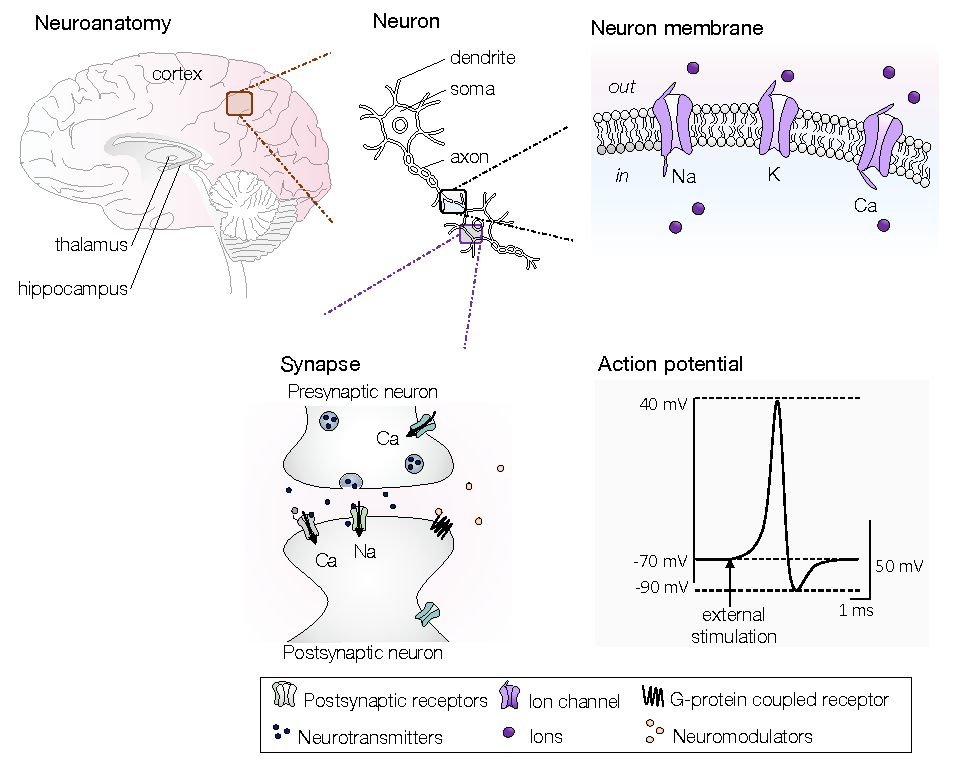
\includegraphics{latex/fig/Intro/Bgd_scale.pdf}
    \caption{Caption}
    \label{fig:Bgd_scale}
\end{figure}

% -----------------------------------
%       Neurons
% -----------------------------------
\subsection{The basics of neuron structure and function}
Our brain is composed of more than 86 billion of neurons \citep{Herculano-Houzel_human_2009}. These fundamental units process the information between the body and the brain. Neurons are excitable that are activated by chemical or electrical signals, and they communicate with one another by generating electrical signals known as \textit{action potential}. Each neuron consists of three main parts: the \textit{dendrite}, which collects the incoming signals, the \textit{soma}, known as the cell body, which integrates these signals and the \textit{axon}, which transmits the response. 

Neurons share similar components with classical cells such as the plasma membrane that separates the intra- and extracellular compartments. This membrane is permeable to small molecules and water, but almost fully impermeable to ions and large molecules. \textit{Ion channels}, which are particular proteins embedded in the membrane, allow the flow of ions through the membrane. They are selective to a given type of ions such as sodium (Na$^+$), potassium (K$^+$), calcium (Ca$^{2+}$) or chloride (Cl$^-$) and they regulate the concentration of these ions accross the membrane. Therefore, the concentration of positive and negative ions on both sides of the membrane and its permeability generate an electrical potential called the \textit{membrane potential}. Without any external signal, the neuron is at its resting potential around \SI{-70}{mV}, which is maintained by the balance of ion concentration and ion channel activity. 

When a neuron receives a stimulus such as stress, pressure, electrical current or chemical transmitters, ion channels open, allowing the flow of ions through the membrane, causing a change in the potential. The neuron responds to this change, by altering its membrane potential. A positive stimulus is increasing the potential, known as \textit{depolarization}, while a negative stimulus decreases the potential, known as \textit{hyperpolarization}. A sufficient depolarization from the resting potential causes the all-or-nothing rise in the membrane potential, corresponding to the \textit{action potential} or \textit{spike}. This also reflects the cell excitability.

% -----------------------------------
%       Ion channels
% -----------------------------------
\subsection{Ion Channels: Their Structure and Role in Neuron Excitability}
Ion channels are membrane proteins that allow the flow of ions following gradient concentration. For example, ions channels allowing calcium flow are called calcium channels. These gateways have specific opening and closing mechanisms that are regulated by complex processes. They can be dependent on the membrane voltage or the calcium concentration. They open or close at different timescales. They can also have blockers that are dependent on other factors. Their kinetics are critical in the regulation of the membrane potential and govern the neuron excitability. Ion channels are complex transmembranic proteins with several substructures that allow the channel opening and closing. These substructures can be described at a more abstract level by visualizing the ion channel with gates; an activation gate or a inactivation gate. Neurons can produce a variety of response thanks to the interplay between the different ion channels that have various gating kinetics and voltage-dependency.


% -----------------------------------
%       Action potential
% -----------------------------------
\subsection{The mechanism of action potential generation}
The most familiar neuronal response is the action potential. At rest, the membrane potential is around \SI{-70}{mV}. When the neuron receives an excitatory stimulus, it depolarizes. If the input stimulus is weak, the neuron will go back to its resting state. If the stimulus is strong, it is activated the choreography of ion flows that builds up the action potential. Sodium channels are voltage-dependent. They allow sodium ions to enter that further depolarize the membrane voltage. Due to the voltage-dependency, more ions are entering and it causes a positive feedback. It creates a rapid depolarization known as the rising phase of the action potential. As the membrane reaches its peak, the voltage-dependent potassium channels open allowing potassium to exit the cell. This repolarizes the neuron on a slower timescale and brings it back to its resting value. The membrane voltage becomes slightly more hyperpolarized than its resting state called the hyperpolarization before it returns to its resting state thanks to the closing of ion channels and the activity of the ion pumps. 

This choreography is governed by the dynamics of sodium and potassium channels. At rest, sodium and potassium activation gates are closed and sodium inactivation gate is open. The excitatory stimulus causes the depolarization of the membrane voltage that causes the fast opening of the sodium activation gate resulting in sodium ion influx. The potassium activation gate is opening but on a slower timescale resulting in potassium ions release after several milliseconds. In parallel, the sodium inactivation gate slowly close stopping the sodium ion influx. The neuron hyperpolarizes causing sodium channel activation gate and potassium channel activation gate to close due to their voltage-dependency and sodium channel inactivation to open again. 

Now that the mechanisms of action potential generation is detailed, the remaining question is how this electrical signal is transmitted to other neurons. 


% -----------------------------------
%       Synapse
% -----------------------------------
\subsection{The Synapse: From Action Potential to Neurotransmitter Release}
When an action potential is generated at the soma, it propagates along the axon. It reaches the axon terminal called the \textit{synapse} and it triggers the release of chemical substances, called the neurotransmitters, to the target neurons. The electrical signal is transformed into a chemical signal. There also exist electrical synapse called gap junction but this thesis focuses on the chemical ones \citep{heidelberger_synaptic_2014}. 

The membrane is depolarized by the arrival of the action potential. It opens the voltage-gated ion channels, allowing calcium to enter the presynaptic neuron and to trigger a signalling cascade. Synaptic vesicles  fuse with the membrane of the presynaptic neurons and releases the stored neurostransmitters in the synaptic cleft. These neurotransmitters bind to the postsynaptic neuron receptors. It generates the opening or closing of these receptors translated by an increase or a decrease of the postsynaptic membrane potential that respectively define an \acrfull{EPSP} or an \acrfull{IPSP}. 
%\textcolor{gray}{Non-neuronal cells such as astrocytes, located near the synaptic cleft, contribute to the neurotransmitter wash-out or regulation \cite{heidelberger_synaptic_2014}}.\\


% -----------------------------------
%       NT & NMOD
% -----------------------------------
\subsection{Neuromodulation: from the definition to its essential and unsolved role in our brain}
\subsubsection{Neurotransmitters vs Neuromodulators: understanding the distinction}
\textit{Neurotransmitters} are chemical substances released by neurons to targeted neurons. There exist different types: \acrfull{NA}, also called norepinephrine, \acrfull{ACh}, \acrfull{5-HT}, \acrfull{DA}, \acrfull{HA} \acrfull{Glu} and \acrfull{GABA}. They target postsynaptic receptors in order to convey the electrochemical signal. In this way, they perform the synaptic transmission.

\textit{Neuromodulators} are a subset of neurotransmitters with a more diffuse release compared to the targeted action of the neurotransmitters during the synaptic transmission. Neuromodulators bind to G protein-coupled receptors and alter the cellular or synaptic properties of the neurons. Instead of carrying the information as performed by neurotransmitters, they can modulate the synaptic transmission by modifying the electrical behavior of the pre- or the postsynaptic neurons. 


\smallbreak
\noindent
\begin{minipage}{0.45\textwidth}
As a brief reminder, two main classes of receptors exist\citep{purves_neuroscience_nodate}. The \textit{ionotropic receptors}, also called called neurotransmitter-gated or ligand-gated channels,  directly open ion channels as soon as the neurotransmitter bind to the protein. The  \textit{metabotropic receptors} are membrane receptors that triggers a cascade of intracellular events using second messenger signal. They are indirectly linked to ion channel regulation.
\end{minipage}
\hfill
\begin{minipage}{0.45\textwidth}
    \begin{shaded}
        Fun fact sur l'histamine
    \end{shaded}
\end{minipage}


% -----------------------------------
%       NMOD: inventaire
% -----------------------------------
\subsubsection{Overview of Major Neuromodulators and their Functions in the Brain}
Neuromodulators play fundamental roles in our brain, and their actions are diverse. However, due to their diffuse effects, it can be challenging to identify their key functions. Moreover, they often work together, as demonstrated by research \citep{gu_neuromodulatory_2002, avery_neuromodulatory_2017, nadim_neuromodulation_2014}. The following is a brief, non-exhaustive overview of the main neuromodulators, categorized according to the location of their generating neurons, their projection regions, and their primary functions.

\begin{figure}[h!]
    \centering
    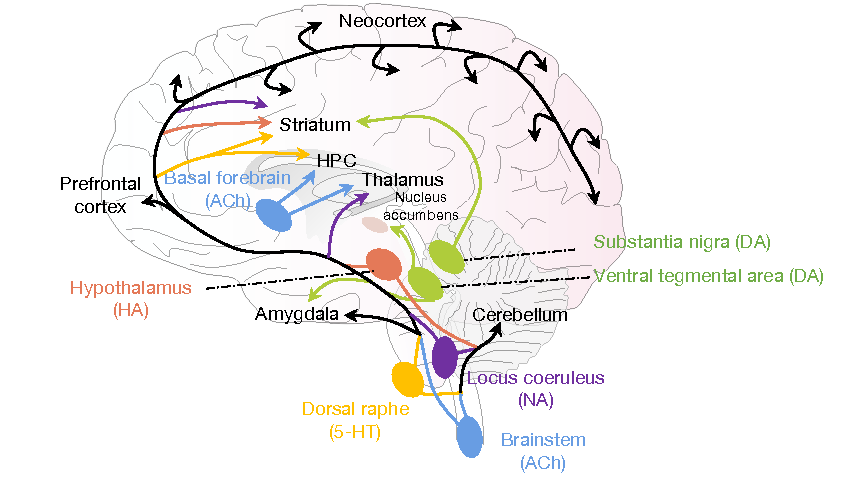
\includegraphics{latex/fig/Intro/Bgd_NMOD.pdf}
    \caption{Caption inspired from \citep{bear_neuroscience_2016, mei_informing_2022}}
    \label{fig:Bgd_NMOD}
\end{figure}

\begin{itemize}
    \item \acrfull{NA}: Noradrenergic neurons are located in the locus coeruleus located in the pons and medulla. They project to the cortex, the cerebellum, the hippocampus, the thalamus, the striatum and the hypothalamus. They are related to arousal and they are mediating vigilance and  alertness.
    \item \acrfull{ACh}: Cholinergic neurons are mainly located in two regions either in the basal forebrain or in the nucleus basalis of Meyner and the brainstem. They are innervating the neocortex,  the thalamus, the hippocampus and the amygdala among others.  There are two types of receptors: nicotinic (ionotropic) and muscarinergic (metabotropic). They could regulate arousal, attention and play a role in play a role in learning,  memory, mood control and behavior control.
    \item \acrfull{5-HT}: Serotonergic are found is in the raphe nuclei of the brainstem. They project to the cortex, hypothalamus, striatum, hippocampus, and amygdala. They play are related to impulsivity, anxiousity, reward or cost assessment as well as learning, memory or sleep. 
    \item \acrfull{DA}: Dopaminergic neurons are located in the midbrain, in the substantia nigra and the ventral tegmental area. They project to the striatum but also to basal ganglia, nucleus accumbens, amygdala, hypothalamus and cortex. This neuromodulator is well-known as the pleasure chemical and its role in the reward system.  It also plays a key role in movement, cognition, motivation, and neuroendocrine control. These dopaminergic pathway plays a critical role in diseases such as Parkinson, schizophrenia and Alzhemeir. 
    \item \acrfull{HA}:  Histaminergic neurons are mainly located in the tuberomammillary nucleus (in the hypothalamus). They have widespread projections in various brain areas including cortex among others \citep{gu_neuromodulatory_2002}. Histamine plays a role in wake-sleep regulation, arousal, motor activity, learning, stress, aggression, pain perception, self-stimulation, reinforcement and other processes listed in \citep{gu_neuromodulatory_2002}.
    \item \acrfull{Glu}: Glutamate is the most encountered excitatory neurotransmitter in the nervous system. Neurons generating glutumate are distributed in the brain. The receptors are either ionotropic such as \acrfull{AMPAr} ($\alpha$-amino-3-hydroxy-5-methyl-4-isoxazolepropionic acid receptor) or metabotropic such as \acrfull{NMDAr} ( N-methyl-D-aspartate). They play a role in the regulation of sleep \citep{watson_sleep_2011}. 
    \item \acrfull{GABA}: GABA is the most encountered inhibitory neurotransmitter. It helps to maintain homeostasis by maintaining an excitatory-inhibitory balance. Neurons realising GABA are also spread in the brain. GABA receptors are either ionotropic, called GABA\textsubscript{A} receptors or metabotropic, called GABA\textsubscript{B}.
\end{itemize}


\subsubsection{Neuromodulation: the Magic Tool in our brain}
\textcolor{red}{Ici ou section suivante}



% -----------------------------------
%       Experimental techniques
% -----------------------------------
\subsection{Tools for Investigating the Brain: from Behavior to Single Neuron Activity}
Neuroscience research relies on a variety of techniques to investigate the function and structure of the brain. These techniques vary in their spatial and temporal resolutions, invasiveness, and technical demands. In the early stage of neuroscience, scientists had not other options than opening the brain and observing the organ, the anatomy and practice surgery \citep{buzsaki_rhythms_2009}. Nowadays, with the development of new technologies, reading the brain from large scale to micro scale has been eased. Here is a non-exhaustive list of the different techniques commonly used in neuroscience:

\newpage
\begin{figure}[h!]
    \centering
    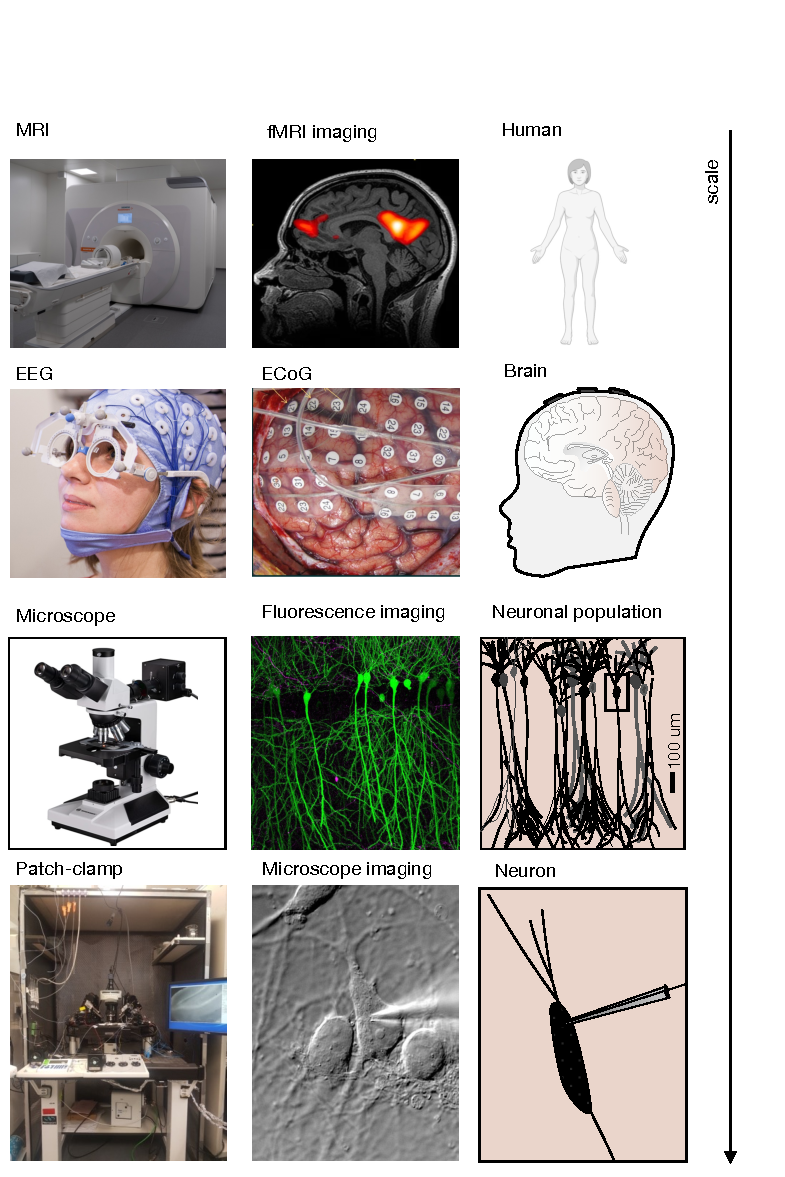
\includegraphics{latex/fig/Intro/Bgd_Tools.pdf}
    \caption{Caption}
    \label{fig:my_label}
\end{figure}



\begin{itemize}
    \item Behavior:\\
    Observing behavior is a simple and technically undemanding technique for gaining insights into human or animal functioning. It can yield valuable information about decision-making, memory retrieval, and sexual behavior among others. Researchers may passively observe behavior or request that participants perform specific tasks. 
    \item Brain imaging - using metabolic activity as indirect mesure of the neuronal activity
    \begin{itemize}
        \item[$\circ$] \acrfull{fMRI}:\\
        Neural activity induces change in metabolic processes such as blood flow or oxygen supply. This non-invasive technique indirectly measures brain activity in different brain regions by detecting variations in blood flow or oxygenation levels. The temporal resolution is not accurate enough to measure rapid changes in brain activity.         
        \item[$\circ$] \acrfull{PET}:\\
        Similar as fMRI, it is a non-invasive imaging technique using radioactive tracers to measuring metabolic activity such as blood flow or glucose uptake for example. 
    \end{itemize}
    \item \acrfull{EEG}:\\
    The EEG is a non-invasive technique using surface electrodes on the scalp. These electrodes record summed activity of large populations of neurons in large brain areas such as population activity of cortical neurons. It is commonly used to study brain rhythms which are associated with different cognitive states. 
    \item \acrfull{MEG}: \\
    MEG measures magnetic fields generated by the neural activity in the brain. Like EEG, it is a non-invasive technique that provides the overall activity of large populations of neurons. It is commonly used to record deeper structures such as thalamus and brainstem. 
    \item \acrfull{ECoG}: \\
    The ECoG is an invasive technique to record population activity of neurons in a large area (order of milimeters square) by placing a grid of electrodes directly at the surface of the brain. It recordes superficial layer of the brain.
    \item \acrfull{LFP}:\\
    Extracellular recording of a population activity of neurons in a localized area of the brain, typicalling using microelectrodes. It reflects the collective activity of populations. It is often used to study neuronal synchrony. 
    \item \acrfull{MEA}:\\
    Cluster of sensors recording up to hundred electrical activity of multiple neurons simultaneously.  
    \item Single neuron recording 
    \begin{itemize}
        \item[$\circ$] extracellular recording: by placing an electrode in the extracellular medium, this technique allows for the recording of sharp variations in the potential but not the membrane potential itself. It is useful for recording the neuronal rhythm. 
        \item[$\circ$] intracellular recording: a sharp pipette is inserted inside the neuron equipped with an electrical sensor to record the electrical activity of individual neurons.
        \item[$\circ$] patch-clamp: similarly as the intracellular recording, a glass pipette is used to create a seal between the pipette and the membrane. This allows the measurement of passing currents through the membrane with high precision. This technique provides a high temporal and spatial resolution but it is invasive and technically demanding. 
    \end{itemize}
    \item Microscope imaging:    \\
    To observe the anatomy of the brain, surgery, dissection and microscope provide inside about morphology of the different structures of the brain from organs to proteins. 
    \begin{itemize}
        \item[$\circ$] Optical imaging: by using a fluorescent substance, calcium concentration can be monitored during the brain or neuronal activity.
        \item[$\circ$]  Calcium Imaging: Calcium levels within the neuron indicating its activity can be recorded by measuring fluorescent dyes. 
        \item[$\circ$] Voltage-Sensitive Dye Imaging: Similarly to the calcium imaging, it uses fluorescent dyes to measure changes in the membrane potential of neurons.
        \item[$\circ$] Two-photon imaging: it is a type of microscopy to record neuronal activity by measuring fluorescent indicators. This device provides a good temporal resolution.  
        \item[$\circ$] Optogenetics: This technique permits to target and control the activity of particular cells by using light-sensitive proteins that are genetically engineering. 
    \end{itemize}

\end{itemize}
Each of these techniques has its own advantages and disadvantages with respect to their spatial or temporal resolutions and its invasiveness. Researchers must carefully choose the appropriate methods to answer their research questions. \\~\\
\smallbreak
\noindent
\begin{minipage}{0.45\textwidth}
\begin{lilashaded}
\textbf{\textit{In-vitro}, \textit{in-vivo} and i\textit{n-silico}}\\
~\\
These terms are sometimes confusing. Here is a brief reminder: \\
- \textit{in-vitro}, translated in glass: the experiments take place in a test-tube.\\
- \textit{in-vivo}, translated  in life: the experiments take place in the living organism. \\
- \textit{in-silico} refers to silicon chip used in computer: the experiments are performed on computers and via virtual simulations. 
\end{lilashaded}
\end{minipage}


\newpage
\begin{figure}[h!]
    \centering
    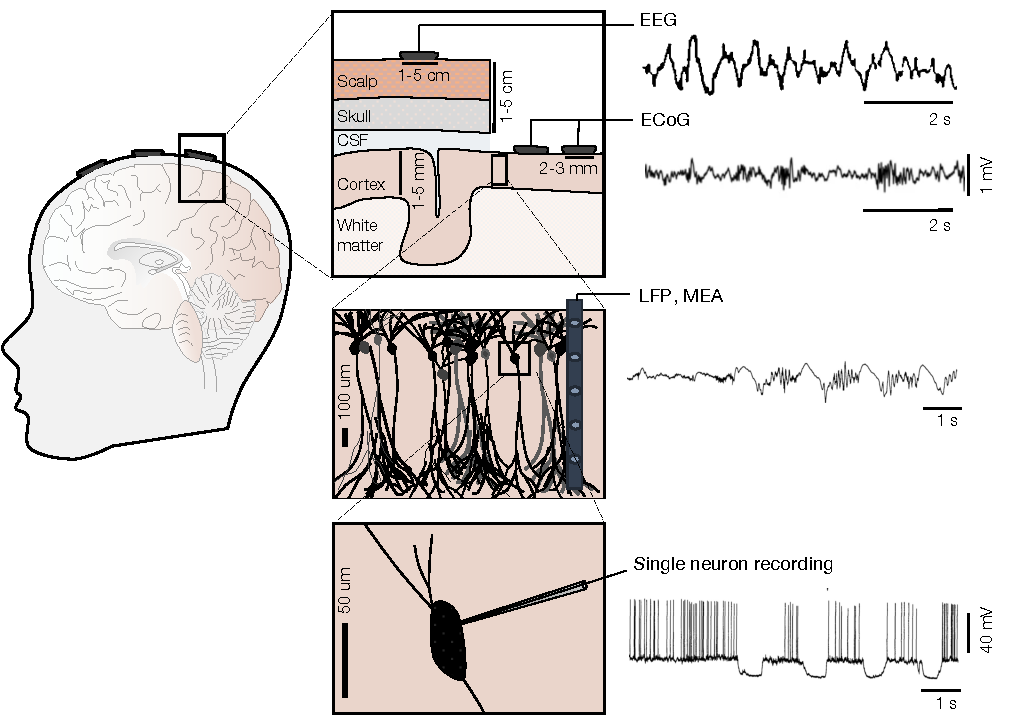
\includegraphics{latex/fig/Intro/Bgd_Recording.pdf}
    \caption{Caption  EEG \textcolor{red}{???}, ECoG \citep{konerding_2018} LFP, Single \citep{steriade_cellular_1995}}
    \label{fig:my_label}
\end{figure}
 



 
\newpage
% -----------------------------------
% -----------------------------------

%     BRAIN STATES
%
% -----------------------------------
% -----------------------------------
\section{Understanding brain states: from brain activity to neuronal activity}

% -----------------------------------
%       Brain state | at the brain level
% -----------------------------------
\subsection{Brain state identification}
Our everyday life is sequenced by different states. During the night, we sleep and dream,  and then we wake up and begin the day. We are capable of walking, looking around, and rapidly reacting to our environment . We can aslo engage in complex actions, think, and remember. These transitions between states are commanded by our brain \citep{bradley_state-dependent_2022}. 

A \textit{brain state} mirrors the overall activity pattern of neuronal population that can vary depending on the context. Indeed, the brain is made of interconnected neurons that communicate with each others, receive information and process it. Ongoing neural activities give rise to rich patterns that can be observed at different scales; from molecule and cell levels to microcircuits or networks up to the whole brain. Capturing brain states at a given spatial scale requires appropriate techniques: from neuronal recordings with pipette to population activity with LFP or EEG. The fluctuations between brain states occur at various timescales. At one extreme, brain states occur at hundreds of milliseconds during sharp shifts of attention, fast memory retrieval or when several action potential are generated in response to sensory stimuli, such as change in light intensity. Intermediatly, brain states are fluctuating in the range of hours with wake-sleep cycles. At the extreme case, brain states evolve over the course of brain development or during long-term changes in behavior, such as skill acquisition or recovery from injury. In the case of the slow progression into degenerative disease, the neural activity is no longer generating the correct brain state.

\begin{figure}[h!]
    \centering
    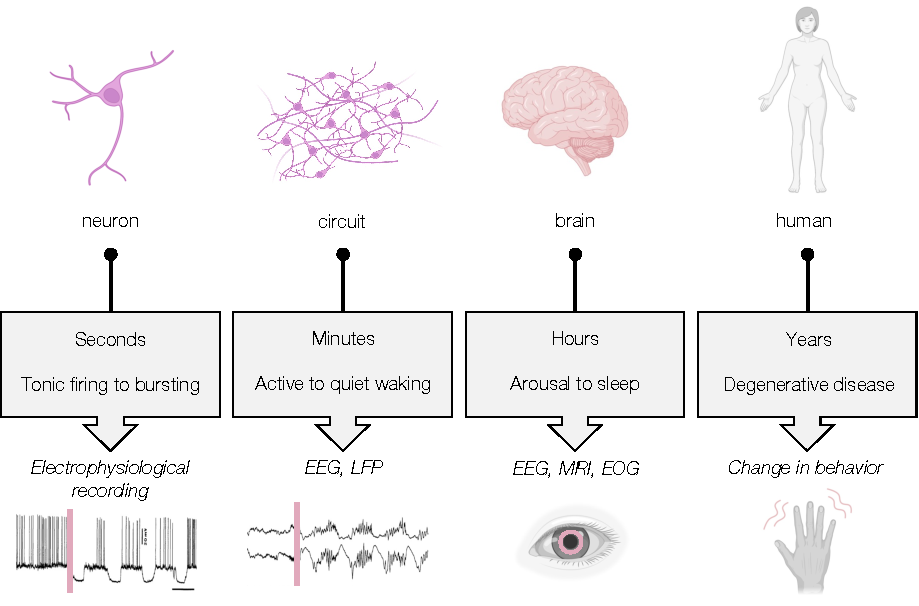
\includegraphics{latex/fig/Intro/Bdg_BScale.pdf}
    \caption{Caption}
    \label{fig:my_label}
\end{figure}

I follow the scientific definition provided in \citep{bradley_state-dependent_2022,zagha_edward_mccormick_neural_2014} telling that a brain state is "a recurring set of neural conditions that is stable for a behaviourally significant period of time. This set of neural conditions is often reflected in distinct patterns of ongoing activity but can also be revealed by neural responses to stimuli." 

Distinct brain states are characterized by distinct neural signatures mostly defined by the frequency and the spatiotemporal patterns of the LFP \citep{kringelbach_brain_2020}. They are often associated to identifiable cognitive or motor states. In addition, other features such as the breathing speed, the muscle tone, the eye movement, the pupil diameter, the heart beat might help to distinguish the brain states \citep{reimer_pupil_2014, mcginley_waking_2015}. 

\subsubsection{Classification and Characteristics of Brain Waves in Different States}
 There exists a large variety of brain waves that were classified based on the frequency content in the EEG or LFP oscillations \citep{tyree_optogenetic_2017}: 
\begin{itemize}
    \item gamma oscillations at 30 to 100Hz - associated with an engaged consciousness.  
    \item beta oscillations at 12 to 30Hz - associated with active waking, concentration and mental alertness.
    \item alpha oscillations at 8 to 12Hz - associated with quiet waking, resting, relaxed and calm state of mind.
    \item theta oscillations at 4 to 8Hz - associated with sleep, deep relaxation or meditation.
     \item delta oscillations at 0.5 to 4Hz - associated with deep sleep, the slowest brain waves.
    
\end{itemize}

\begin{wrapfigure}{r}{0.5\textwidth}
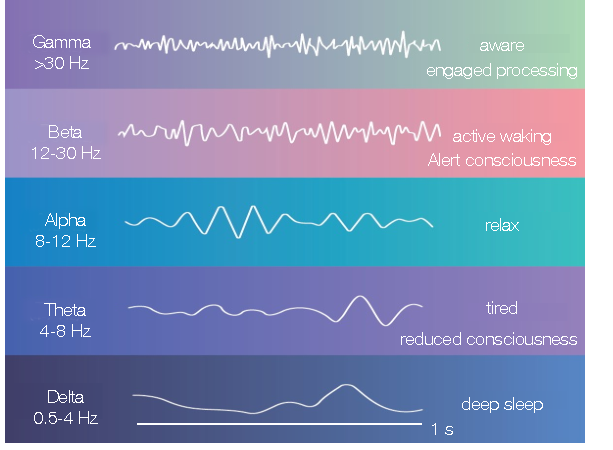
\includegraphics[scale=0.75]{latex/fig/Intro/Bdg_BrainWaves.pdf}
\caption{...}
\label{fig:BrainWaves}
\end{wrapfigure}

The familiar example of sleep helps to get more insight about the fluctuations in brain states \citep{mcginley_waking_2015, molnar_cell_2021} Classically, deep sleep is characterized by a large-amplitude and low-frequency signal with no eye movement and reduced muscle tone, referred as \acrfull{NREM}, associated with a succession of delta and theta oscillations). By opposition, waking is associated to small-amplitude faster frequency fluctuations (associated to a mixture of alpha and beta oscillations). These two stages are often described respectively as a global synchronization dominated by low frequency content or global desynchronization.  The term \acrfull{REM} is often encountered for the dream stage that looks similar as the waking state except paralyzed muscle tone and rapid-eye-movement are observed. 

This simplistic distinction between waking and sleep have been challenged and the concept of active and quiet waking have been introduced. During waking, larger-amplitude, lower-frequency oscillations are observed for example in the somatosensory, visual, and auditory cortical regions. They are associated to quiet waking. These oscillations are suppressed as soon as human or animals enter active waking due to for example motion or attention shift \citep{mcginley_waking_2015}. 


\subsubsection{Fluctuations in brain states}
The brain's evolution during a given action or mindset is a fascinating phenomenon, as is understanding how the transition between different states occurs. For instance, when we are meeting someone important, our heart rate increases, our hands sweat, and our body temperature rises, all of which are orchestrated by the brain operating in an alert state. Various pathways, such as brain circuitry, movement-related factors, and breathing, influence the transition between states \citep{tantirigama_perspective_2020}. However, neuromodulation is the major factor that affects the transition. Figure \textcolor{red}{XXX} provides insight into the close relationship between brain states and neuromodulators. The cocktail of chemical substances is constantly fluctuating. During active waking, the brain has a high concentration of acetylcholine, noradrenaline, serotonin, dopamine, and histamine. These concentrations decrease in quiet waking and are very low during \acrfull{NREM} sleep.

Several diseases, such as schizophrenia, epilepsy, autism, Alzheimer's, and Parkinson's disease, dramatically alter brain states \citep{uhlhaas_neural_2006, kuhn_event-related_2004, cannon_neurosystems_2014}. Parkinson's disease, for instance, is often recognized by motor dysfunctions such as arm tremors, which is explained by a drastic change in the expected brain state. \textcolor{red}{add image of brain state switches with the figure}

The mechanisms underlying switching between brain states are not yet fully understood. Studying the interplay between neuromodulation and switches in brain states at the cellular level can provide insight into these mechanisms.




\begin{figure}[h!]
\hspace{-1cm}
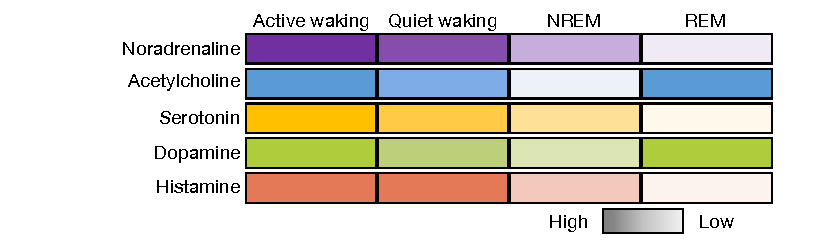
\includegraphics[scale=1]{latex/fig/Intro/Bgd_NMODinBS.pdf}
\caption{ .... 
Inspired by \citep{tyree_optogenetic_2017} }
\label{fig:intro_tyree_opto}
\end{figure}

 

% -----------------------------------
%       Brain states: at the neuron level
% -----------------------------------

\subsection{Neuronal activity reflects the brain state}

The diversity of neurons in the brain is what allows for the myriad of brain states that we experience. Neurons come in different morphology, shapes and sizes, and possess unique types of ion channels which allow them to generate electrical signals and communicate with other neurons. Their different neuronal properties allow them to generate firing pattern. \textit{Firing pattern} refers to the way the neuron produce an action potential over time.  It depends on the neuron itself as well as the timing and the intensity of the received stimulus. The term neuronal excitability is often encountered in literature and refers to the ability of a neuron to generate an action potential in response to a stimulus.



\subsubsection{Classification of neuronal firing patterns}
Figure \textcolor{red}{XXX - tous les firing patterns} uncovers the existence of the different firing patterns often encountered. This is a non-exhaustive list and description of these patterns \citep{komendantov_quantitative_2019, izhikevich_classification_2004}:
\begin{itemize}
    \item \textit{tonic firing}: the neuron produces a succession of action potentials in response to an external stimulus or a sustained input (also called tonic spiking, regular spiking).
    \item \textit{bursting}: the neuron generates a sequence of clustered action potential occuring at high frequency separated by silent periods \citep{kucyi_neural_2017}.
    \item \textit{pacemaking}: the neuron generates a constant succession of action potentials at a fixed frequency independently of any external input, only by relying on its intrinsic properties.
    \item \textit{adapting spiking}: the generates a succession of action potentials with a gradual decrease in their firing rate over time in response to a constant stimulus.
    \item \textit{plateau potential}: the neuron can maintain its spiking activity for a relatively long period of time after the occurence of an excitatory stimulation, it is a form of bistability \citep{marder_plateau_2003}.
    \item \textit{rebound burst}: burst of action potentials in response to an hyperpolarization input.\\
\end{itemize} 

The Blue Brain project engages in a gargantuan challenge: the reconstruction and simulation of a column of the neocortex. They model different cell types classified based on their morphology and their firing patterns  \citep{markram_reconstruction_2015}.  I decided to focus my interest in two firing patterns: tonic spiking and bursting. 


\begin{figure}[h!]
    \centering
    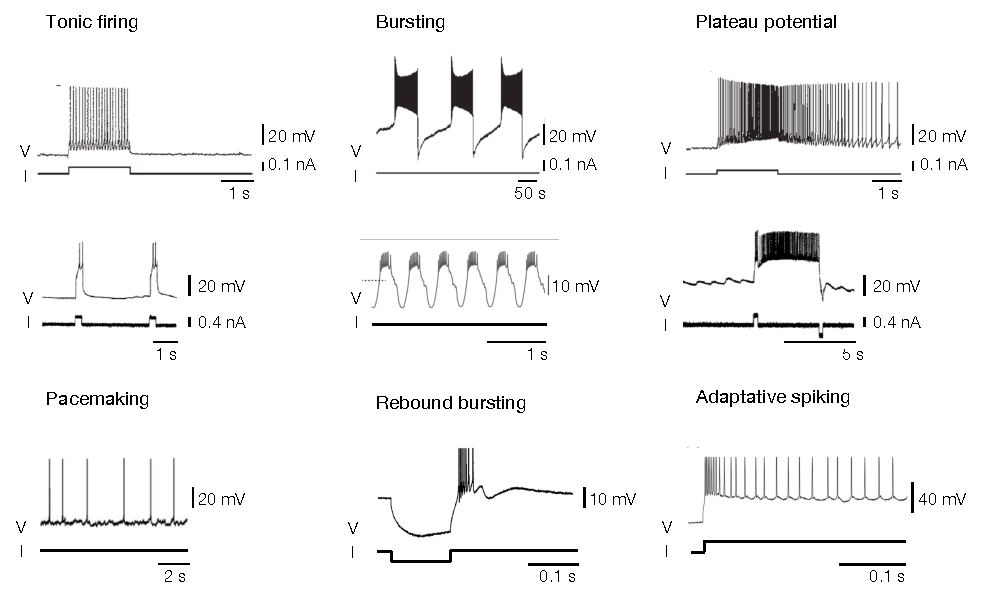
\includegraphics{latex/fig/Intro/Bgd_FiringPattern.pdf}
    \caption{Tonic (dorsal \citep{marder_plateau_2003}, DG \citep{weimann_effects_1993}), Burst (dorsal \citep{marder_plateau_2003}, lateral pyloric \citep{marder_from_2021}),  Pacemaking (\citep{ramirez_role_2011}, Plateau (dorsal \citep{marder_plateau_2003}, DG \citep{weimann_effects_1993}  }
    \label{fig:my_label}
\end{figure}

\begin{comment}
\begin{figure}
    \centering
    \includegraphics{fig/Intro/Izhikevich_classification}
    \caption{"Summary of the neuro-computational properties of biological spiking neurons [Izhikevich, 2004]. This figure is re- produced with permission from www.izhikevich.com. (Electronic version of the figure and reproduction permissions are freely available at www.izhikevich.com)." \citep{izhikevich_classification_2004}}
    \label{fig:intro_izhikevich}
\end{figure}
\end{comment}

\subsubsection{Bursting: Definition, Characteristics, Shape, and Mechanisms of generation}
Already investigated 25 years ago, this firing pattern was defined by "clusters that often last at most \SI{25}{ms} and contain several action potentials from two to 6 at a high frequency (about \SI{200}{Hz})" \citep{lisman_bursts_1997}. The interest for this particular firing pattern has continued to grow. 
~\\
\textit{Brain regions containing neurons able to burst}\\
Bursting is observed in several brain regions  \citep{shao_neural_2021, zeldenrust_neural_2018} such as in the cortex, mostly in pyramidal neurons, in the hippocampus, in the pyramidal neurons in CA1 region, the thalamus, in the thalamocortical and neurons of the reticular nucleus, in the hypothalamus, in gonadotropin-releasing hormone (GnRH)  neurons, in the cerebellum, in purkinje and granules cells,  in the brainstem, in the ventral tegmental area, in dopaminergic neurons. It is also observed outside the brain and in different species such as in pre-Botzinger complex - in the respiratory neurons, in stomatogastric ganglion in crustaceans - in anterior bursting neuron, in abdominal ganglion in aplysia - in neuron R15,  in circuit involved in central pattern generator \citep{grillner_CPGs_2021}, in pancreatic beta cells \citep{jeong_bursting_2012}. 

~\\
\textit{Bursting are characterized by several features}\\
Bursting can be described by different features \citep{van_pottelbergh_robust_2018, drion_novel_2012} 
\begin{itemize}
    \item The \textit{active period} is the duration composed of the succession of action potentials, called the burst or spike train. 
    \item The \textit{quiescent period} is the silent period between the spiking period, also called intraburst interval.
    \item the \textit{intraburst period} is the timing between two distinct burst of action potential. 
    \item the \textit{intraburst frequency} is the inverse of the intraburst period. 
    \item the \textit{interburst period} is the timing between two action potentials inside the burst, also called inter-spike interval. It can vary within the burst. 
    \item the \textit{interburst frequency} is the inverse of the interburst period. 
    \item the \textit{duty cycle} is the ratio between the intraburst period and the interburst period. 
    \item the number of \textit{\acrfull{SPB}}.
    \item the \textit{spike latency} is the delay between the start of the depolarization and the start of the spike train.
    \item the \textit{plateau} potential: the burst of action potentials occur at a more depolarized potential than the hyperpolarized state. It allows to identify an up and down state in the firing pattern. 
    \item the \textit{\acrfull{ADP}} the burst is finished by a small depolarization bump before hyperpolarizing.
\end{itemize}



~\\
\textit{Bursting can take several shapes}\\
Bursting can display different signatures that are described by the oscillations \citep{desroches_classification_2022, drion_novel_2012, van_pottelbergh_robust_2018, smith_fourier_2000}: 
\begin{itemize}
    \item  the \textit{parabolic bursting}: the train of spikes is at a noticeable depolarized state with respect to the hyperpolarized membrane voltage. It is observed in Aplysia R15 for example \citep{adams_slow_1985, turrigiano_selective_1995}
    \item the \textit{square wave bursting}: the neuron discharges continuslouly during the active period and stop without a noticeable plateau potential. It is observed in pancreatic beta-cells \citep{bertram_phantom_2008} but it is more often encountered in mathematical models. 
    \item the \textit{elliptic bursting}: the burst is a bit more depolarized compared to the parabolic bursting observed in sensory neurons.
    \item the \textit{pseudo-plateau bursting}: a strong plateau potential is observed and the amplitude of the successive action potentials in decreasing. 
\end{itemize}

~\\
\textit{Mechanisms behind bursting}\\
Two categories of burst generation are considered according to \citep{jeong_bursting_2012,jeong_bursting_2012} : 
\begin{itemize}
    \item forced burst generation: the burst is the consequence of stimulation with a current that drives the neuron above or below the action potential threshold. This current can be the result of either an external simulation via an electrode - for example a square-wave signal current or synaptic input. In the case of synaptic input, either the neuron is normally spiking but a periodic inhibitory provokes intervals of silence or the neuron is silent and receives periodic excitatory synaptic input causing the clusters of action potentials (see Figure \ref{fig:intro_burst}) 
    \item intrinsic burst generation: the neuron is able to burst due to the different ion channels. Their opening and closing kinetics orchestrate the intrinsic generation of bursting such that intrinsic currents depolarizes the neuron until it reaches its firing threshold, allowing the occurrence of several action potentials. Then, the neuron hyperpolarizes on a ultraslow timescales. This sequence is repeated due to the interaction of the different ion channels. Experimental neuroscientists have been trying to identify the ionic currents necessary in this autonomous pattern generation. The T-type calcium channels have been recognized to play an important role \citep{cain_contributions_2010} (see Figure \ref{fig:intro_burst}) . 
\end{itemize}



\begin{figure}[h!]
    \centering
    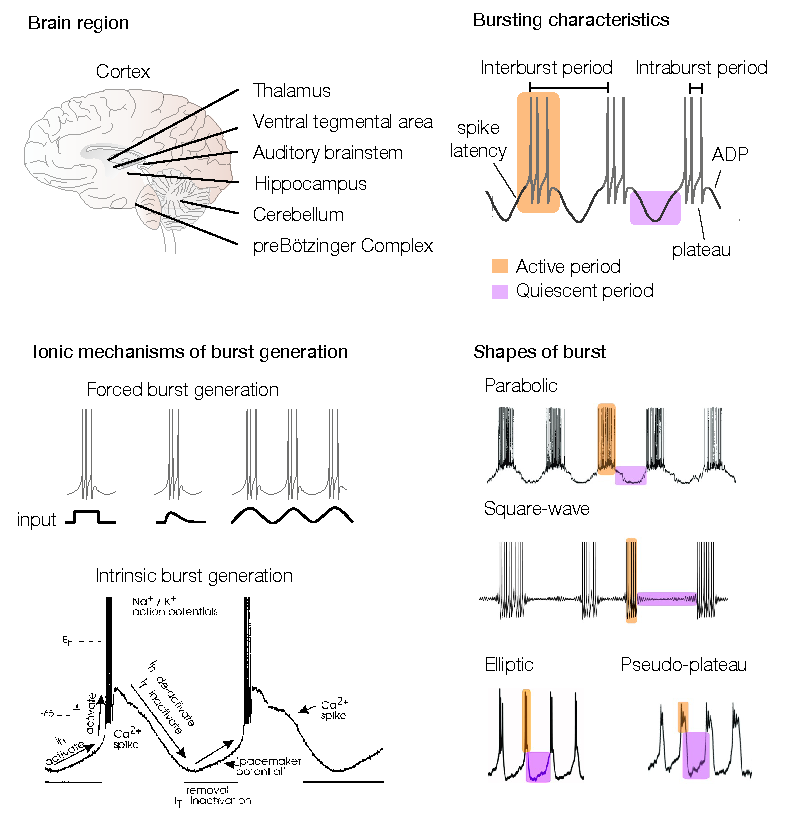
\includegraphics[scale=1]{latex/fig/Intro/Bgd_Burst.pdf}
    \caption{\citep{zeldenrust_neural_2018, desroches_classification_2022, mccormick_sleep_1997}}
    \label{fig:intro_burst}
\end{figure}

~\\
\newpage
\subsubsection{Neurons are able to switch between firing patterns}
Neurons are fundamental units of the brain; their variety in morphology, roles and now their firing patterns is at the basis of the complexity and power of our  brain.  Figure \textcolor{red}{XXXX} shows that firing pattern vary from one neuronal population to the other. But most surprisingly, one neuron can switch from firing pattern to an other firing pattern. It is mainly caused by the modulation of ion channel properties. Several factors can modulate these properties such as:
\begin{itemize}
    \item neuromodulation (like dopamine, serotonin or acetylcholine): neuromodulators alter the ion channels for example by blocking or recruiting them, changing their densities, altering their kinetics \citep{steriade_novel_1993}. 
    \item synaptic input: a inhibitory input can switch a neuron from regular spiking to bursting by activating some ion channels that were previously closed. 
    \item environmental changes: temperature and pH among others are external factors that can modify the ion channels \citep{hedrick_effect_2012} (see Figure \ref{fig:intro_switch} XXXX)   
    \item other mechanisms such as change in the resting potentiel or changes in the extracellular concentration of potassium \citep{frohlich_coexistence_2006}.
\end{itemize}


\subsubsection{Switches from tonic spiking to bursting}
\textit{Mechanisms at the cellular level}\\
The thalamic neuron has been a nice support since many years to understand what are the key mechanisms between the transition from tonic spiking to bursting \citep{mccormick_sleep_1997, cain_contributions_2010} (see Figure \ref{fig:intro_switch}\textcolor{red}{XXX}).  This neuron is mainly driven by sodium current, potassium current, T-type calcium current and hyperpolarization-activated current (H current). At a depolarized state, the neuron is governed by the dynamics of the sodium and potassium channels generating succession of action potentials. Due to change in the neuromodulatory state for example, the neuron is hyperpolarized that results in calcium channels. They open in a slow timescale generating a calcium influx that depolarizes the neuron (see Figure \textcolor{red}{XXXX}). Sodium and potassium current interplay to produce action potentials. Simultaneously, calcium channels close on a ultraslow timescale. The neuron hyperpolarizes, no more action potential is generated. The hyperpolarization-activated current enters into account to depolarize the neuron and activate the whole process again. 

To switch from tonic spiking to burst, the neuron must be hyperpolarized to allow the activation of calcium channels. As explained earlier in the mechanisms of switches, this can be achieved by applying an external hyperpolarized current or neuromodulators affect the ion channel properties and set the neuron in a hyperpolarized state. \\
~\\
~\\
\textit{Switching from tonic spiking to bursting is not only associated to transitions from wakefulness to sleep}\\
The switch from tonic spiking to bursting is drastically impacting the brain states as earlier explained that neuronal activity is shaping these states \citep{takahashi_neuronal_2006}. This section is explaining the relationship between this switch at the cellular level into the switch in brain state and the associated behavioral state. 

The switch from tonic spiking to bursting is often associated to the transition from wakefulness to sleep. Indeed, during wakefulness, neurons are reacting to incoming signals and discharges accordingly in tonic spiking. This is translated at the population level by a small, high-frequency signal. Transitioning to sleep, neurons are bursting, a synchronization of the activity is created resulting in a large, low-frequency LFP signal \citep{mccormick_sleep_1997}. It is often encountered to talk about active (up) and inactive (down) periods occurring at low frequency. Tonic mode was thought to be the default mode during wakefulness to relay the information while bursting mode was associated to a blocking of the information from the external mode. 

But more and more evidence confirms that bursting occurs during wakefulness \citep{fanselow_thalamic_2001, steriade_natural_2001, zagha_edward_mccormick_neural_2014, reimer_pupil_2014}. Some recordings were even obtained in monkey \citep{guillery_thalamic_2002} while in the past it was mainly on rodents and cats. Bursting plays a role in the information processing during waking behavior \citep{sherman_tonic_2001,ramcharan_burst_2000}. This is explained by the presence of slow oscillatory activity during quiet waking with absence of movement. As soon as the animal walks, the slow rhythmic activity is suppressed \citep{mccormick_brain_2015}. "While the slow oscillation was once thought to be restricted to periods of slow wave sleep, animal studies now suggest that it may occur in the waking state, particularly during periods of inattentiveness or drowsiness"
 
These switches in wakefulness have an impact on sensory processing \citep{steriade_natural_2001}. This bidirectional switch allows to meet changing behavioral demands \citep{crandall_corticothalamic_2015}. 

~\\
\textit{Examples from Dopaminergic Neurons, Sensory Processing, and Neurological Diseases}\\
This section provides several examples of switches from tonic firing to bursting and their corresponding switches in brain states and behavior. 

Dopaminergic neurons have three modes of discharge: pacemaking, phasic or bursting \citep{tsai_phasic_2009, johnson_burst_1992}. Without stimulation, the neuron is in pacemaking mode. It fires at a small frequency around \SI{1}{Hz}. During a stimulation, the frequency increases during the applied input. Finally, under special conditions, neurons is bursting. The switch from regular spiking to bursting is observed in paradoxal slep and palatable food consumption \citep{dahan_prominent_2007, ji_tuning_2009}. 

Neurons in the cortex are sensitive to drugs like ketamine. \citep{cichon_ketamine_2023} observed that drugs can trigger 'non-ordinary brain states' by suppressing the spontaneous activity of some neurons and activating some silent ones. The brain enters a particular mode in which it is disconnected of the external environment but still performing internal subjective experiences \citep{cichon_ketamine_2023, yang_ketamine_2018}. 

We have the ability to switch from hearing to listening. It is translated by a switch in brain states mirroring the switch in neuronal activity in the auditory cortex and other brain regions \citep{de_franceschi_task-induced_2021}. It is confirming that sensory inputs in this case sound is processed in different manners depending on the neuronal firing patterns. This state-dependent sensory processing also occurs in the olfactory cortex \citep{murakami_state-dependent_2005}. Response to smells is bigger while neurons are spiking compared to the weaker response while neurons are in low-frequency rhythm. 


Some diseases are marked with pathological brain states. As mentioned earlier, parkinson or alzheimer diseases are well-known examples of abnormal brain oscillations compared to normal conditions. In normal conditions, neurons in the subthalamic nucleus (STN) neurons and globus pallidus (GP) neurons are in tonic activity - characterized by an small amplitude, high frequency content at the population level. In abnormal conditions (in PD), the STN and GP are in low-frequency rhythmic bursting \citep{bevan_move_2002, beurrier_subthalamic_1999}. In the context of dystonia - a neurological disease that causes the muscles to contract involuntarily, purkinje cells that were tonically spiking in control conditions exhibit a abnormal high-frequency bursting \citep{fremont_abnormal_2014}. For pain processing, depending on the operation mode of the neuron: the pain is differently processed by our brain. In spiking mode, the innocuous stimuli are associated to acute nociception, while the generation of plateau potentials, by increasing the excitability of deep dorsal horn neurons plays a role in central sensitization \citep{marder_plateau_2003}. To illustrate with a simple example, the contact with a needle can be interpreted by three sensations: either pain is only felt when the needle touches the skin (spiking mode), or pain persists after the needle removal (plateau potential mode) or pain is abnormally felt even without simumus (bursting mode). There are also examples in the context of anxiety, depression epilepsy, schizophrenia, addiction among others. Better understanding the modification of discharge patterns could help to develop therapeutic treatments. 



\begin{figure}
    \centering
    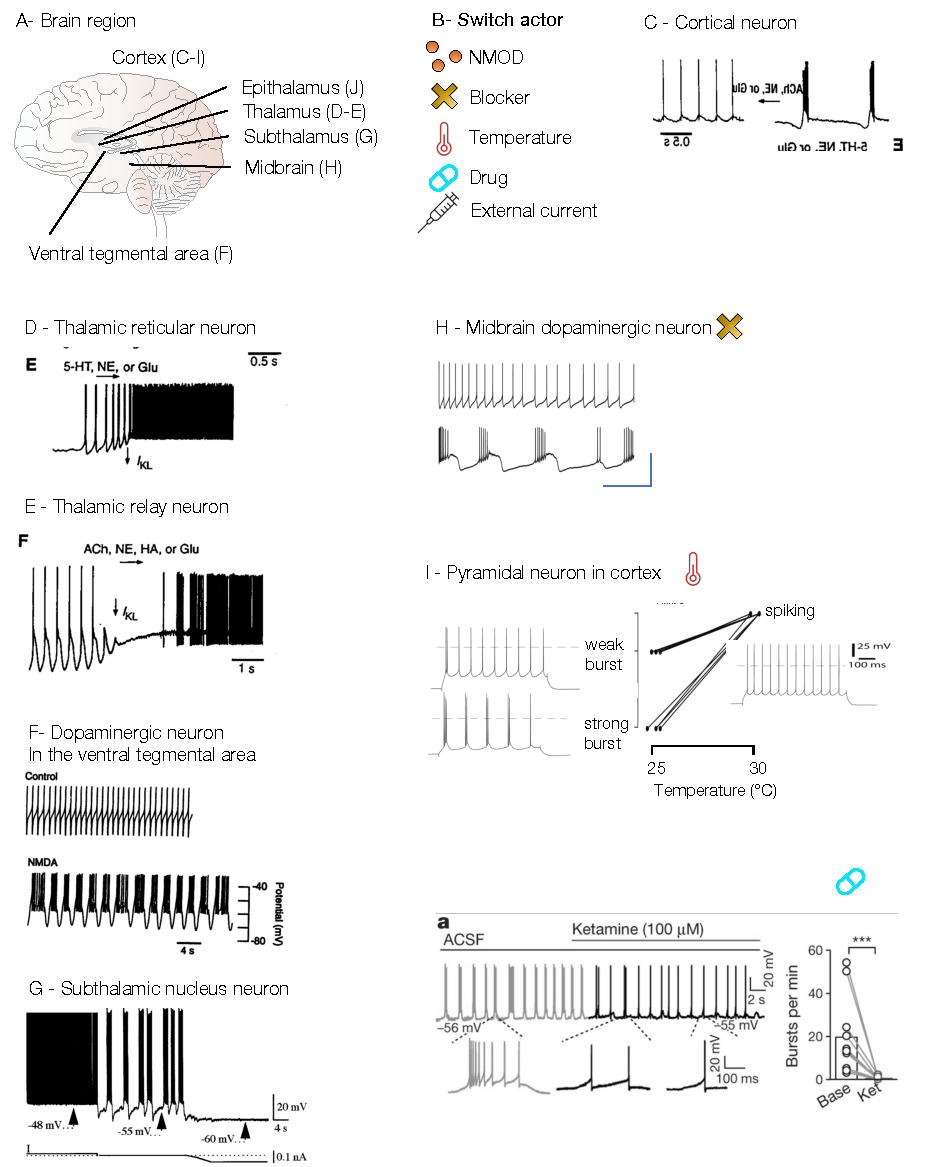
\includegraphics{latex/fig/Intro/Bgd_Switch.pdf}
    \caption{\citep{mccormick_sleep_1997, ji_tuning_2009, johnson_burst_1992, hedrick_effect_2012} McCormick (anesthesized cat), Ji (rats), Jonhson (), T (mice), Cichon (rodent ket), Yang (rodent ket- artificial cerebrospinal fluid , Locomotion (Polack), Wake-sleep (Steriade 2001)) \textcolor{red}{retravailler l'ordre de l'image: montrer les deux neurons thamalamiques en mettant aussi le behavior puis montrer des switches dans le cortex eveil sommeil/locomotion puis DA neurons puis Temperature et drug)}}
    \label{fig:intro_switch}
\end{figure}

Yang: "but completely eliminated spontaneous burst firing within seconds of application"
\begin{comment} --- le texte est bien formulé ---
"Neural oscillations are a hallmark of cortical network dynamics (Buzsaki and Draguhn, 2004). Sustained oscillatory activity can be broadly classified as either tonic firing or bursting. Neurons in a number of brain structures including the thalamus (Jahnsen and Llinas, 1984a,b) and neocortex (McCormick et al., 1985; Connors and Gutnick, 1990) exhibit either tonic firing or bursting in a state-dependent way. One of the most dramatic examples of global transitions between bursting and tonic spiking regimens is the transition from slow-wave sleep to rapid eye movement sleep or waking in the thalamocortical system (Steriade et al., 1993, 2001; Timofeev et al., 2001; Steriade and McCarley, 2005). Slow transitions between a slow-wave state and a fast-wave state were also observed in the olfactory cortex (Murakami et al., 2005). Coexistence of bursting and tonic spiking regimens is not limited to vertebrates (Lechner et al., 1996; Turrigiano et al., 1996; Shilnikov et al., 2005). Different levels of synaptic excitatory drive, activation of intrinsic conductances by neuromodulation, and changes in the extracellular ionic environment control the state-dependent oscillatory regimen" --- >MODEL (bazhenov)\\
\end{comment}


\newpage
\section{Neuromodulation: link between switches in neuronal activity, brain states ...}
\textcolor{red}{Décider si on met la neuromodulation ici ou au dessus}


\begin{pinkshaded}
Neuromodulators are powerful substances in our brain that control and allow us to rapidly react. Their mechanisms are complex due to their diffuse projecting and their broad operating modes. Figure~\ref{fig:Bgd_NMOD} confirms that studying the effects of neuromodulators is a real struggle due to their multiple targets and their coordinated actions. 

Aa smart strategy to investigate neuromodulation is to move to small circuit as done in the impressive work of Eve Marder. Crustaceans have well-defined neuron circuits and are multiply modulated \citep{marder_understanding_2007}.

Neuromodulators affect the neuron circuit by changing the frequency, the number of spikes per burst so that a same circuit can display several output patterns. The mechanisms underlying these changes have investigated in the last 30 years \citep{nadim_neuromodulation_2014, marder_understanding_2007}: 
\begin{itemize}
    \item One neuromodulator may affects different voltage-gated ion channels.
    \item Individual neuromodulators may have different actions on a neuron by altering different physiological mechanisms .
    \item Different neuromodulators may have a converging action on a same voltage-gated ion channels.
    \item Neurons and synapses are affected by neuromodulators. 
\end{itemize}

(...) It rises the question of how is it possible to alter as many parameters and simultaneously maintain a network output. 

~\\
----\\
back to the future\\

Then the effects of descending modulatory projection neurons on the STG are removed by either cutting or blocking the input nerve to the STG, the fast pyloric rhythm either stops completely or slows down (Figure 3, control). Under these conditions, exogenous application of a large number of different substances can elicit a triphasic motor pattern


effect of DA: \\
An unexpected result from this work is that dopamine modulates several currents in the same neuron and that the same current can be modulated differently in different target neurons


Understanding how circuits can be stable in the face of ubiquitous neuromodulation is an important and deep problem.
stability mechanisms 1) si un NMOD jour sur un courant inward et outward, le resultat va etre le meme. 


Can Modulator Action Be Robust and Predictable Despite Variability in Underlying Conductances? Much computational and experimental evidence shows that there can be considerably variability across animals or across neurons in the parameters that control neuronal excitability and network function even when the circuit output is maintained

\end{pinkshaded}



\begin{figure}[h!]
    \centering
    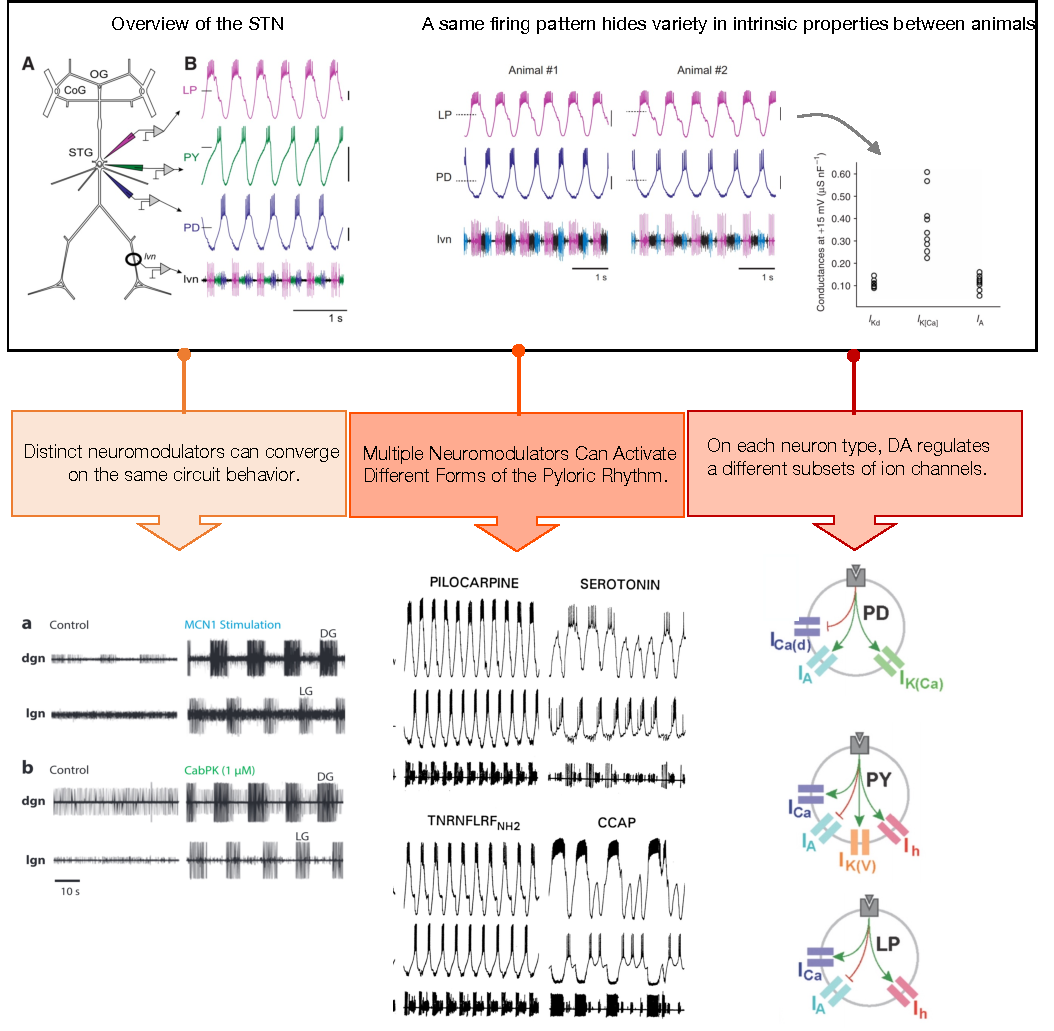
\includegraphics{latex/fig/Intro/Bgd_Marder.pdf}
    \caption{Diagram \citep{marder_neuroscience_2021}, conductance distribution \citep{schulz_variable_2006}, (bottom-left)  \citep{marder_neuromodulation_2014} (bottom-middle) \citep{marder_neuromodulation_2012}  (bottom right) \citep{marder_understanding_2007}}
    \label{fig:my_label}
\end{figure}

\newpage
~\\
\newpage
% -------------------------
% -------------------------
%
%     SYNAPTIC PLASTICITY
%
% -------------------------
% -------------------------
\section{Synaptic plasticity}

\begin{comment}
Our neurons have the ability to modify their connections with each other, a property called \textit{synaptic plasticity}. 
According to \citep{citri_synaptic_2008}, it refers "to the activity-dependent modification of the \textit{strength} or \textit{efficacy} of synaptic transmission" at synapses \citep{citri_synaptic_2008}. 

Before digging further into the concept of synaptic plasticity, it appears mandatory to introduce the different concepts of  synaptic transmission, synaptic strength or synaptic efficacy among others.
\end{comment}
\textcolor{red}{INTRO}

\subsection{Synapse: definition, structure and functioning}
The term \textit{synapse} originates from Greek sunapsis, from 'sun' that means together and 'hapsis' that means joining from the verb 'haptein', in total it gives joining together. It corresponds to the junction where information is transmitted. It consists of the presynaptic terminal (the end of an axon), the gap between the two neurons (synaptic cleft) and the postsynaptic neurons that contains receptors (dendritic spine). 


The \textit{synaptic transmission} corresponds to the ability of neurons to transmit the information between each other. An action potential generated at the presynaptic neurons reaches the axon terminal and it is converted into a chemical signal that corresponds to neurotransmitter release. These neurotransmitters bind to the postsynaptic neurons that generate a response. The \textit{synaptic strength} refers to the magnitude of this synaptic response that can be recorded as an \acrfull{EPSP} or \acrfull{EPSC} (for excitatory synapse).  In the literature, the terms synaptic strength and synaptic efficiency are interchangeable, while the synaptic strength reflects the response magnitude, the  \textit{synaptic efficiency} defines how well a synapse transmits information. 

The synaptic strength can be increased or decreased and it is what makes our brain plastic and able to adapt the connections between neurons. Before exploring all the plasticity mechanisms, a more accurate description of the synaptic transmission and the synapse is required.







\subsubsection{Synaptic transmission}
The information transmission consists in three main steps as shown in Figure \ref{fig:SP_SynTrans}: (i) the action potential at the presynaptic neuron is triggered  glutamate release, (ii) glutamate binds to the postsynaptic receptors, (iii) the postsynaptic receptors allow flow of ions inside the postsynaptic neurons that generate a change in the postsynaptic membrane voltage.\\
~\\
\begin{wrapfigure}{l}{0.4\textwidth}
 \centering
    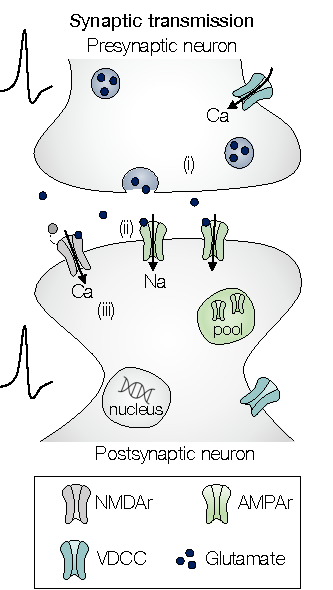
\includegraphics[scale=0.8]{latex/fig/Intro/SP_SynTrans.pdf}
    \caption{caption}
    \label{fig:SP_SynTrans}
\end{wrapfigure}
(i) The membrane depolarization at the presynaptic neuron terminal allows calcium to cross the membrane which trigger a signalling cascade. Synaptic vesicles containing neurotransmitters fuse with the membrane and release the stored neurotransmitters in the synaptic cleft 

~\\
(ii) Glutamate bind to two postsynaptic receptors that perform distinct roles in both synaptic  transmission and synaptic plasticity.  The first of these receptors is \acrshort{AMPAr}, an ionotropic receptor that opens when glutamate binds to it. Once activated, sodium and potassium ions primarily flow through the membrane, resulting in a increase in the postsynaptic membrane voltage. The second type of receptors is the \acrshort{NMDAr}, which is a metabotropic receptor that opens under two conditions, namely when glutamate binds to it and the magnesium blockage is removed. This removal of the blocker enables ion flow through the channel when the membrane voltage is sufficiently depolarized. This receptor are primarily selective for calcium ions, but also allow sodium and potassium ion flow. 

~\\
(iii) Both \acrshort{AMPAr} and \acrshort{NMDAr} work together to mediate synaptic transmission. Glutamate released from the presynaptic neuron binds to both receptors, but only opens the \acrshort{AMPAr}, resulting in ion flow and membrane depolarization. This depolarization triggers the removal of magnesium blocker, allowing \acrshort{NMDAr} to open, as the two activation conditions are fulfilled. The \acrshort{NMDAr} are often called coincidence detector as its activation requires a presynaptic activity causing glutamate release and a postsynaptic activity causing depolarization to remove Mg2+ block. Calcium flows into the postsynaptic neurons.



As I will add more details below, calcium plays a crucial role in the process of synaptic plasticity and it is why it is really important to understand how and why it enters the postsynaptic neuron.  Another source of calcium entering the postsynaptic neurons is voltage-dependent calcium channels such as L-type or T-type among others \citep{lamprecht_structural_2004}. These calcium channels can amplify the depolarization. 

Finally, the postsynaptic neuron responses to the presynaptic neuron action potential. It can be measured by the \acrfull{EPSP} or \acrfull{EPSC} \citep{citri_synaptic_2008}.


\subsubsection{Details on the spine composition}
As just described, postsynaptic receptors are principal actors in the synaptic transmission. They are located at a particular region of the postsynaptic neurons: on the \textit{spine}. 

The dendritic spine is a small protrusion at the surface of the dendrite that receives the input from other neurons (see Figure \ref{fig:SP_spine}A). It consists in a thin neck and a spine head. The dendritic spines contains receptors, channels, signalling molecules, which are useful for its functional role and protein scaffolds, which provide the spine structure \citep{bozelos_impact_2017}. These receptors, basically \acrshort{AMPAr} and \acrshort{NMDAr}, are concentrated at the tip of the spine in a visually distinct site called the \acrfull{PSD} \citep{bonilla-quintana_can_2022}.

The spine morphology is characterized by several geometric features: the length and the width of the neck, the volume of the head, the surface area of the \acrshort{PSD}. These features are correlated with the number of postsynaptic receptors as well as the readibility of transmitter pool, resulting in the efficacy of the synaptic transmission  \citep{Borczyk_neuronal_2019}.

Based on these features, spines can be classified into three categories (see Figure \ref{fig:SP_spine}B): (1) filopedia is a finger-like spine, (2) thin spine, (3) mushroom spine and (4) stubby spine. Logically, spines with a larger head and a larger propose a stronger connection between the pre- and the postsynaptic neurons \citep{bonilla-quintana_can_2022, lamprecht_structural_2004}. The spin shape relies on the spine cytoskeleton, composed with \textit{actin} filaments.  

The spine has the ability to compartmentalize calcium influx that empowers it with a input-specific property. \\

\begin{figure}[h!]
    \centering
    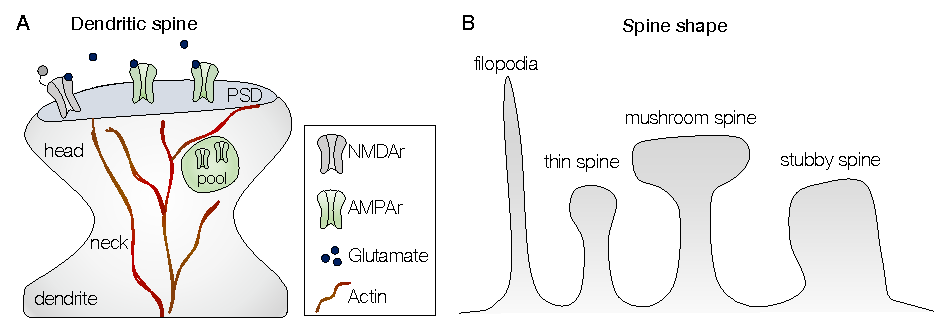
\includegraphics[scale=0.9]{latex/fig/Intro/SP_Spine.pdf}
    \caption{Caption}
    \label{fig:SP_spine}
\end{figure}



\subsection{Plasticity: from early to late change }
How do neurons adapt their synaptic strengths with each other or in other words, how do synaptic plasticity work ?  This is Scientists are  \citep{takeuchi_synaptic_2014}. Ramon y Cajal proposed theoretical hypotheses about the change in synaptic transmission in the mid-twentieth century \citep{cajal_estructura_1888}. Followed by Donald Hebb that brought attention about plasticity with his famous quote "cells that fire together, wire together" \citep{hebb_organization_1949}. Experiences on Aplysia provide some of the first evidence that synaptic strength change in response to stimuli \citep{kandel_behavioral_1979}. In parallel, \citep{bliss_long-lasting_1973} who introduced the notion of \acrfull{LTP} and \acrfull{LTD}, a a form of long lasting synaptic plasticity. \acrshort{LTP} involves a persistent increase of synaptic strength, while \acrshort{LTD} involves a persistent decrease of synaptic change \citep{lamprecht_structural_2004}. 

Nowadays, researches on synaptic plasticity is exploding; from understanding the molecular mechanisms to the formation of new networks. It confirms that synaptic plasticity can be described by many forms and mechanisms and that is also region-dependent. It can span from miliseconds to hours, days and even longer \citep{citri_synaptic_2008}. I will first recall what are the different quantitative measures of plasticity, the different tools used to record plasticity and what are the most encountered plasticity-induced protocols. Then, I will enter the core of the plasticity mechanisms from short-term plasticity to longer-lasting synaptic changes.  

%\textcolor{gray}{Synapses are formed by two partners: a presynaptic and a postsynaptic neurons. Synaptic plasticity is likely to emerge from joint effects of both pre- and postsynaptic processes \citep{poirazi_love_2017}.}
%+ \textcolor{red}{est-ce que je liste les différentes "potentiels acteurs/mechnanisms ? >> faire un tableau? }



\subsubsection{Quantification of synaptic plasticity}
There are several ways to quantitative how the synaptic transmission is modified \citep{cirelli_sleep_2017}. Here is a non-exhaustive list: 
\begin{itemize}
    \item at the structural level: change in spine size, axon to spine interface (ASI), spine volume, spine width;
    \item at the molecular level: change in the number of synaptic receptors such as AMPAr;
    \item at the electrophysiological level: change in \acrshort{EPSP} or \acrshort{EPSC} (by comparing the amplitude \citep{bi_synaptic_1998} or the change in slope \citep{frey_effects_1993}), the  evoked responses, unit firing.
\end{itemize}

\subsubsection{Tools to measure synaptic plasticity}
Synaptic change can be monitored at the the structural level by modern imaging technologies; by tracking the evolution of the spine morphology. Change in \acrshort{EPSP} or \acrshort{EPSC} are recorded by electrophysiological recording for example via electrodes in the postsynaptic neurons \citep{abraham_is_2019}. The advantages and disadvantages of the different techniques are discussed in  \citep{glasgow_approaches_2019}. 




\subsubsection{Plasticity-induced protocols}
Experimentalists record one of these quantities mentioned above to define a basal control condition ($w_0$). Then, perform a plasticity-induced protocol. After the protocol, the same quantity is measured and the ratio provides the synaptic change ($\Delta w$). Figure \ref{fig:SP_STDP} explains the different steps achieved in electrophysiology to provide experimental data after a plasticity-induced protocol \citep{bi_synaptic_1998} 
%In computational models, the initial weight is given by $w_0$ and after the experiment, the synaptic change is defined by $\Delta w$.


\begin{figure}[h!]
    \centering
    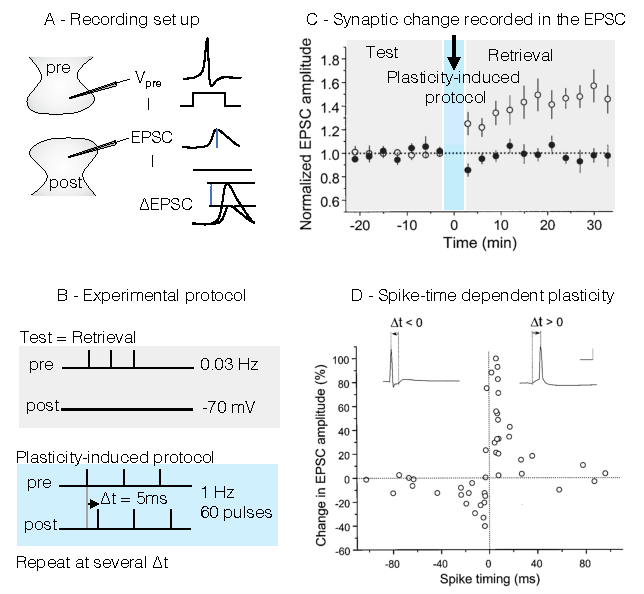
\includegraphics[scale=1]{latex/fig/Intro/SP_STDP.pdf}
    \caption{Caption \citep{bi_synaptic_1998}}
    \label{fig:SP_STDP}
\end{figure}

Figure \ref{fig:SP_Protocols} (top) provides an overview of the most common plasticity-induced protocols performed in the last years \citep{krieg_unifying_2014}. The strategy is to test the effect of one parameter onto the synaptic strength: such as the presynaptic frequency, the timelag between two pre and postsynaptic spikes ($\Delta t$), the postsynaptic membrane voltage $V_{\mathrm{post}}$ among others.
\begin{itemize}
    \item  the \textit{rate protocol} records the synaptic strength after exciting the presynaptic neuron at a given frequency while the postsynaptic is resting ($ \Delta w =F(f_{\mathrm{pre}}) $) \citep{dudek_homosynaptic_1992, frey_synaptic_1998, gerstner_hebbian_2011}.
    \item The \textit{Spike-Time Dependent Plasticity} protocol is largely used; the pre- and postsynaptic neurons are stimulated a low frequency (0.1 or 1Hz) with a certain timelag $\Delta t$ ($\Delta w =F(\Delta t$) \citep{debanne_asynchronous_1994, bi_synaptic_1998, markram_regulation_1997, abbott_synaptic_2000, gerstner_neuronal_1996}.
    \item The membrane \textit{voltage} of the postsynaptic neuron is affected the result of the rate-protocol ($\Delta w =F(V_{post}, f_{pre}$) \citep{bi_synaptic_1998, artola_different_1990, sjostrom_rate_2001, ngezahayo_synaptic_2000, artola_long-term_1993}.
     The \textit{frequency}-dependent protocol consists in generating spikes at a given pairing frequency ($f_{pairing})$  with presynaptic spikes preceding postsynaptic spikes by 10 ms (or post-pre with a time delay written -10 ms) ($\Delta w =F(f_{pairing}$ with $\Delta t = \pm 10 $ms)\citep{sjostrom_rate_2001}.
     \item \textit{More complex} induction protocols were designed. Triplet and quadruplets are similar as the STDP protocol, three or four spikes are generated instead of two have \citep{wang_coactivation_2005, froemke_spike-timing-dependent_2002, froemke_contribution_2006, wittenberg_malleability_2006}. Postsynaptic 'bursts':  repetitive action potentials in a short period of time of 1, 2 or 3 spikes paired with one single presynaptic spike induced experimentally in the cortex \citep{nevian_spine_2006, debanne_asynchronous_1994,froemke_contribution_2006}.
\end{itemize}
More details on plasticity induced protocols are available in \citep{inglebert_synaptic_2021, krieg_unifying_2014}. More factors can influence the result of the synaptic plasticity such as the synaptic location \citep{froemke_spike-timing-dependent_2002, sjostrom_cooperative_2006} and more indirect factors such at the initial synaptic strength \citep{ngezahayo_synaptic_2000}. 

\begin{figure}[h!]
    \centering
    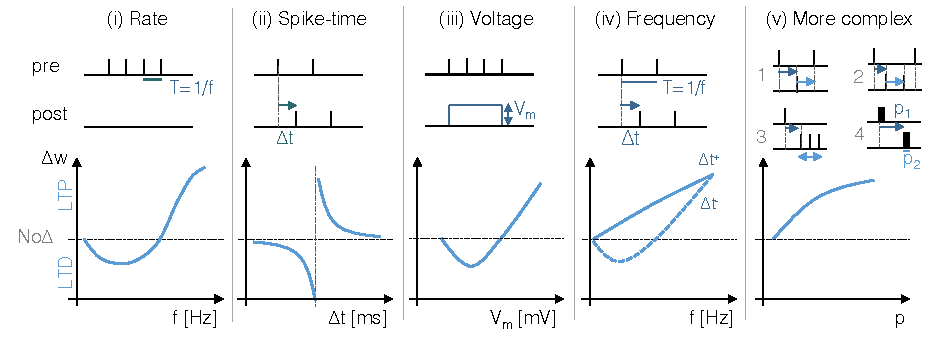
\includegraphics[scale=0.9]{latex/fig/Intro/SP_Protocols.pdf}
    \caption{Caption}
    \label{fig:SP_Protocols}
\end{figure}



\subsubsection{Short-term plasticity}
Short-term plasticity refers to changes in the synaptic transmission that occurs over a period ranging from miliseconds to several minutes. There are two types of short-term plasticity: facilitation and depression. Briefly, \textit{facilitation} involves an increase in the synaptic strength due to the rapid succession of action potentials at the presynaptic neuron \citep{castro-alamancos_distinct_1997}  This activity leads a buildup of residual calcium, which in turn  affects the exocytosis of synaptic vesicles resulting, in the change in probability of the neurotransmitter release \citep{citri_synaptic_2008}. In contrast, \textit{depression} involves a decrease of the synaptic strength caused by the depletion of neurotransmitter stores at the presynaptic terminal \citep{heidelberger_synaptic_2014}.

Short-term plasticity is often correlated with mechanisms at the presynaptic neurons while longer changes in the synaptic plasticity preferentially occur at the postsynaptic neuron. 



\subsubsection{Long-term plasticity: definition and classification}
\acrfull{LTP} was shown experimentally (exactly 50~years ago) by\citep{bliss_long-lasting_1973} as a long-term increase in the synaptic strength following a brief, high-frequency stimulation or other induction protocol \citep{baltaci_molecular_2019}. Nowadays, we define \acrshort{LTP} more globally as activity-dependent long-lasting increase in the synaptic strength \citep{abraham_is_2019, citri_synaptic_2008}. Fourty years ago,  \acrshort{LTP} was already divided into two categories depending on the generation of new proteins or not as shown experimentally in  \citep{frey_effects_1993, krug_anisomycin_1984} by using inhibitor of protein-synthesis.

\begin{itemize}
    \item \acrfull{E-LTP} refers to the early phase of long-term change, which is independent of protein synthesis, without any structural of the synapse. It lasts up to 1-3h.
    \item \acrfull{L-LTP} refers to the late phase, which is dependent on de-novo protein synthesis (with the activation of transcription factors) and structural change of the synapse.
\end{itemize}
Conversely, the concept of \acrfull{LTD} refers to long-lasting decrease in the synaptic strength. In the quest of unrevealing the mechanisms behind these long-term changes, the causal steps of the induction and the maintenance are recalled. It starts with the calcium influx inside the postsynaptic neuron that will trigger a signalling cascade. I will dissect this cascade to identify how plasticity occurs. 



\color{black}
~\\

\subsubsection{Mechanisms of early long-term potentiation (E-LTP) and depression (E-LTD)}
We need to zoom at the molecular level to understand the machinery.  Calcium enter the postsynaptic neuron and binds to calmodulin, forming the complex known as \acrfull{CaM}. This complex acts as a dynamic calcium sensor, depending on the concentration, it triggers differ processes that either lead to \acrfull{LTP} (for elevated calcium influx) or \acrfull{LTD} (for intermediate calcium influx) \citep{kotaleski_modelling_2010, feldman_spike-timing_2012, seibt_primed_2019}. Figure \ref{fig:SP_E-LTP} details their mechanisms. 

~\\
\textit{\acrfull{E-LTP}}\\
In the case of elevated  calcium influx, the calcium/calmodulin (CaM) complex triggers calcium/calmodulin dependent protein kinase, known as CaMK (see Figure \ref{fig:SP_E-LTP}A). A \textit{kinase protein} has the property to regulate other proteins by attaching phosphate groups, a process known as phosphorylation, which causes functional change in the targeted protein \citep{bear_neuroscience_2016, seibt_primed_2019}. In the context of synaptic plasticity,  CaMKII, a member of the CaMK family,  is known to phosphorylate a variety of proteins, including ion channels, neurotransmitter receptors, and synaptic scaffolding proteins. One of its most important targets is the \acrshort{AMPAr}. As previously explained, it is the primary mediator of fast excitatory synaptic transmission in the brain. Elevated calcium influx quickly activates CaMKII, which potentiates the synapse by two manners: 
\begin{itemize}
    \item (i) increase in existing \acrshort{AMPAr} efficiency via phosphorylation leading to a better synaptic transmission.
    \item (ii) insertion of new \acrshort{AMPAr} into the postsynaptic membrane - a process known as fast AMPAr trafficking.  Indeed, some vesicles queue near the membrane, and in response to \acrshort{CaMKII} activation, the vesicles filled with new \acrshort{AMPAr} fuse with the membrane and deliver new \acrshort{AMPAr} to the synapse, via exocytosis, causing the swelling of the spines \citep{seibt_primed_2019}.  
\end{itemize}
The \acrfull{E-LTP} is independent on de novo protein synthesis and morphological change of the spine. 

\begin{figure}[h!]
    \centering
    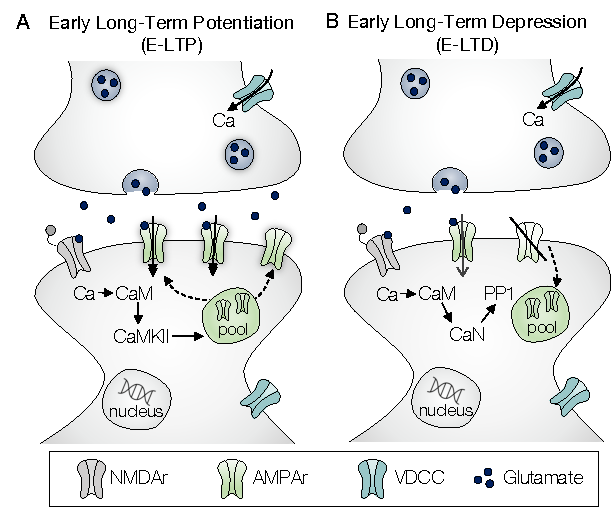
\includegraphics{latex/fig/Intro/SP_E-LTP.pdf}
    \caption{Caption}
    \label{fig:SP_E-LTP}
\end{figure}

~\\
\textit{\acrfull{E-LTD}}\\
In the case of intermediate calcium influx, the \acrfull{CaM} triggers calcium/calmodulin-dependent protein phosphatase, known as \acrfull{CaN} (see Figure \ref{fig:SP_E-LTP}B). A phosphatase protein is an enzyme that removes phosphatase from target proteins. This, in turn, activates another phosphatase protein called \acrfull{PP1}, which inhibits the action of CaMKII by dephosphorylating it \citep{citri_synaptic_2008}. 

As previously explained, calcium is crucial for synaptic plasticity, which raises the question of how a same signal can trigger \textit{both} LTP and LTD ? The key difference lies in the level of NMDAr activation, and it is important to remember that the different types of calcium response selectively activate different types of enzymes that have opossing effect. LTP and LTD reflect the bidirectional regulation of the phosphorylation and the number of AMPAr. \\ 



\subsubsection{Mechanisms of late long-term potentiation (L-LTP) and depression (L-LTD)}
The \acrshort{LTP} that lasts longer and induces changes in the spine morphology refers to \acrfull{L-LTP}. It is distinguished from \acrshort{E-LTP} by its protein synthesis. Figure~\ref{fig:SP_L-LTP} illustrates the mechanisms. 

On a longer timescale, the rise of calcium level that activates \acrshort{CaMKII} or CaMKIV (another member of the CaMK family) in turn activate \acrfull{cAMP} \citep{golbert_sleep_2017}. This  intracellular signaling molecule activates protein kinase A (pKA) (see Figure~\ref{fig:SP_L-LTP}A). Then, this latter enters the nucleus and activates transcription factors such as \acrfull{CREB} that regulates gene expression. These transcriptions factors can induce the expression of gene that encode new proteins, including \acrshort{AMPAr} and growth factors.  After the synthesis of new \acrshort{AMPAr}, they are trafficked to the synapse, via slow AMPAr trafficking. Additionally, the growth factors modify the synapse morphology and the cytoskeleton is impacted by modifying some support-protein such as \textit{actin}.  by Altogether, it contributes to the long-term morphological change such as for example enlargement of spine head (larger surface, increase in spine head volume, spine neck widening and shortening), growth of the dendtric spines (polymerization of actin filament), insertion of new receptors that were synthetized (by contrast to the fast trafficking of new receptors from the available vesicles pools), formation of new synapses, rearrangement of actin cytoskeleton and changes in the distribution of neurotransmitter receptors (receptor clustering).

Figure~\ref{fig:SP_L-LTP}B shows microscope imagine of a dendritic spine growth. The generation of new protrusions and the increase in volume of existing spines are clearly depicted \citep{lamprecht_structural_2004}.  The complementary process of \acrfull{L-LTD} triggers another signalling cascade that promotes the removal and inhibition of \acrshort{AMPAr} and the shrinkage of the spine \citep{bliss_long-term_2011}.

This level of details is sufficient for the purpose of my thesis for more information on the  intracellular signaling pathways see \citep{berridge_calcium_2014, citri_synaptic_2008, kotaleski_modelling_2010, bading_nuclear_2013, heidelberger_synaptic_2014,golbert_sleep_2017, seibt_primed_2019, feldman_spike_2020}.

\begin{figure}[h!]
    \centering
    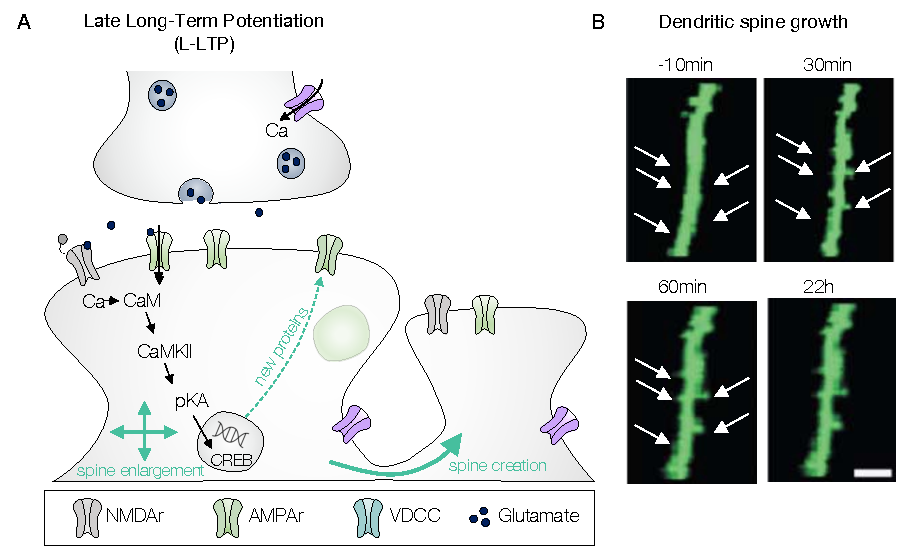
\includegraphics{latex/fig/Intro/SP_L-LTP.pdf}
    \caption{Caption \citep{lamprecht_structural_2004}}
    \label{fig:SP_L-LTP}
\end{figure}




\subsubsection{E-LTP, E-LTD, L-LTP, L-LTD, induction, expression, maintenance ... Clarificiation of the diverse concepts }

In my pursuit of understanding how neurons alter their connections with each other, I first reviewed synaptic transmission. Next, I distinguished between short-term and long-term changes, and then classified long-term changes into two categories based on the generation of new proteins: early and late processes. I also detailed the causal steps that mediate lasting changes at the synapse.

Figure \ref{fig:SP_Summary} presents a schematic overview of what I will refer to as \textit{traditional synaptic plasticity} and \textit{structural synaptic plasticity}. The terminology in this field can be overwhelming, but I aim to summarize the various concepts in a concise manner and present the hypothesis of my thesis.

The process known as \acrfull{E-LTP}, or \textit{LTP expression} \citep{heidelberger_synaptic_2014}, involves the exocytosis of new AMPAr from the vesicle pool and an increase in the efficacy of existing receptors, without any protein synthesis or spine morphological changes \citep{lamprecht_structural_2004}. In computational neuroscience, it is often associated with the \textit{traditional plasticity rule}.

In contrast, \acrfull{L-LTP}, or \textit{LTP maintenance} \citep{heidelberger_synaptic_2014}, involves an increase in the number of receptors in a given spine, changes in the efficacy of existing receptors, and even more characterizing of this phase, the morphological changes in the spine \citep{lamprecht_structural_2004}. The generation of new proteins mediates this process, and in computational neuroscience, it is often modeled by the \textit{structural plasticity rule}.

In both situations, \acrshort{AMPAr} are likely to be inserted or remove from the postsynaptic membranes but the insertion mechanism is different dependent the \acrshort{LTP} category. During \acrshort{E-LTP}, new receptors are inserted at the postsynaptic membrane from pools of available receptors. By contrast, for \acrshort{L-LTP}, the insertion of new receptors requires first its production thanks to protein synthesis. 

Many factors complicate our understanding of synaptic plasticity, such as presynaptic transmitter release or gene activation \citep{baltaci_molecular_2019, citri_synaptic_2008}. Neuromodulators are also likely to affect several factors in different ways. Further studies on plasticity at the molecular, neuronal, and population levels are necessary to gain a better understanding of learning and memory, and eventually provide guidance for related diseases.







\begin{figure}[h!]
    \centering
    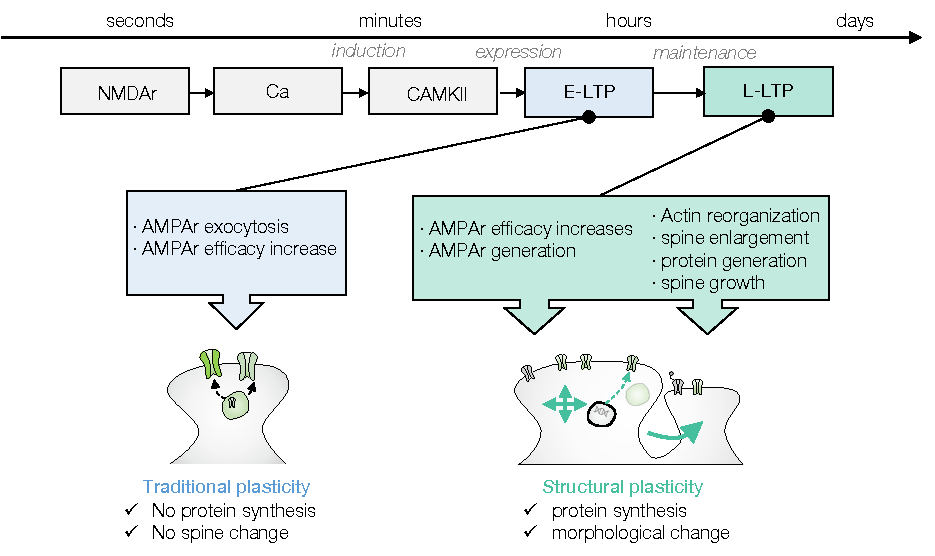
\includegraphics{latex/fig/Intro/SP_Summary.pdf}
    \caption{Caption}
    \label{fig:SP_Summary}
\end{figure}


\newpage
~\\
\newpage
\color{gray}
\subsection{Further mechanisms}

\textcolor{red}{PARAGR à rédiger à la fin  quand on conclu }
\subsubsection{Memory is dynamics}
To conclude this section on synaptic plasticity, it is important to note that memory is stored on synapses that are dynamically regulated. Ongoing plasticity of connections empowers animal and human to live, learn and react on a dynamic environment \citep{abraham_is_2019}. Additionally, there is more and more evidence that memory is not fixed forever on a given network, naming for example memory drift \textcolor{red}{REF}. Memory also involves consolidation between different brain regions as described in the theory of active memory consolidation \citep{born_sleep_2006}.

\subsubsection{Intrinsic plasticity}
Another type of synaptic plasticity really relevant at the circuit level is intrinsic synaptic plasticity \citep{daoudal_long-term_2003, debanne_plasticity_2019, sehgal_learning_2013}. It is defined as change in intrinsic property of a neuron like change in the number of density of ion channels.

bio: \citep{debanne_spike-timing_2010}

\subsubsection{Synaptic-Tagging and Capture Hypothesis}
This hypothesis proposes that only tagged synapses can used \acrfull{PRP} that are necessary for \acrshort{L-LTP} \citep{baltaci_molecular_2019, abraham_is_2019}.

\textcolor{red}{A voir si on laisse ici ou si on explique ca dans la review}


\subsection{NMOD OF SP}
\citep{frey_effects_1993} "L-LTPcome from thefindingthatL-LTPisblockedbyantag- onistsofdopaminereceptors"


"Modulatory neurotransmitters such as dopamine (DA), noradrenaline (NA), serotonin (5-HT) and acetylcholine (ACh), which act on their respective receptors to activate cAMP-dependent signaling in neurons,41-44 also play a role in regulating the longevity of synaptic plasticity. Broadly speaking these neurotransmitters serve as physiological effectors of reward, punishment, arousal and attention, all brain-states that modulate the longevity of memory."


article bio: \citep{lisman_neohebbian_2011, lerner_neuromodulatory_2011}\\
~\\


\color{black} 
\begin{comment}
\color{black}
\begin{wrapfigure}{r}{0.45\textwidth}
    \centering
    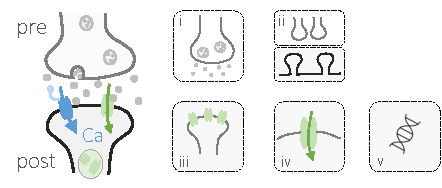
\includegraphics[scale=1]{fig/Intro/PlasticityType.pdf}
    \caption{\textit{Long-term synaptic plasticity expression.} \\
    \textcolor{cyan}{la figure est juste la pour montrer comment faire un wrap figure}
    \\In white boxes, changes concerning the presynaptic site. In light gray, changes concerning the postsynaptic site. From left to right: change in probability of neurotransmitter release, change in volume and number of dendritic spines, change in AMPA receptors number, change in receptor conductance and gene expression.  \textcolor{red}{adapter la légende + la figure sur base de Lamprechts 2004 super belle fig 1 + fig 2}}
    \label{fig:SP_PlasticityType}
\end{wrapfigure}
\end{comment}

\begin{comment}
\newpage
\color{gray}
\subsubsection{Vocabulary}

 memory engram \\
lire: \citep{choi_interrogating_2022} Recently, several studies verified the electrophysiological properties of the engram synapses. Engram synapses showed higher neuronal excitability and AMPA/NMDA ratio compared to other neurons [13,35]. If potentiation between engram cells had already occurred, it was difficult to have additional synaptic enhancements [36]. Even though the direct visual observation of synapses between the engram cells was not performed, it provided the physiological characteristics and functional changes of engram connections. Neuronal ensembles of engram cells distributed throughout the brain form functional neural networks [37, 38, 39]. Since the synapses that constitute this network eventually become the functional units that can subserve the functional roles of neurons, future investigations should incorporate the functional consequences with any interrogation of the physiological and structural relevance of such analyses.\\
\citep{} Memory formation and storage relies on structural changes that occur in the connectivity between neurons. Richard Semon, an early advocate of a physical theory of memory, was the first to term the neural substrate containing memories as the memory engram (Semon, 1904; Schacter, 2001). He defined the engram as the lasting modification produced by experience and stimulation in the brain. Attempts in the 20th century to find and identify the engram were intense\\
    GPT: A memory engram is a specific pattern of neural activity that represents a particular memory. It is thought that memories are encoded in the brain by creating specific engrams, which can be reactivated to retrieve the memory.\\
    ~\\
    \textit{Synapsogenesis} refers to the process by which new synapses are formed between neurons. %This process is critical for the development and plasticity of neural circuits, and it is believed to be a key mechanism underlying learning and memory.}

\color{black}
\end{comment}



 \begin{comment}
 >>> intro bien écrite pour un article 
 
\citep{choi_interrogating_2022}\\
 To form a network, neurons communicate with other neurons via synapses, and each synapse has its own functional properties depending on the presynaptic neurotransmitter and specificity of postsynaptic receptors. Various types of receptors are expressed at synapses in a neuron, indicating that multiple types of neurotransmitters are received as inputs – excitatory, inhibitory, or modulatory. As an example, amygdala pyramidal cells receive excitatory inputs from hippocampus and cortex, form inhibitory connections with neighboring interneurons, and even receive neuromodulatory inputs from the ventral tegmental area (dopamine) and dorsal raphe (serotonin) [9,22, 23, 24]. 
 (...) 

 The synapse, as the functional unit of neurons, is not a fixed structure, but rather undergoes constant changes by various stimuli. External stimuli activate neurons across the brain, and these activities induce structural/functional changes at the synapse, known as synaptic plasticity [25, 26, 27]. The most well-known functional synaptic plasticity is long-term potentiation (LTP), defined as persistence of synaptic strengthening, and is a key concept in learning and memory. LTP was first identified in the hippocampus in 1973 by Bliss and Lomo [28,29] and has since been verified by other methods through numerous studies thereafter [30,31]. This conserved principle has been extended to recent studies on engram cells, which have utilized diverse investigations of LTP in engram cells .

 \end{comment}


\begin{comment}
Just below,  the biological mechanisms underlying LTP and LTD are briefly described. The regulation of AMPAr are introduced such as their insertion or removal or their change in conductance \citep{bading_nuclear_2013, seibt_primed_2019, golbert_sleep_2017, berridge_calcium_2014}. NMDAr might also be dynamically regulated \citep{ferreira_co-agonists_2017}. The maintenance of the synaptic changes is explained by the change in gene expression and new proteins synthesis triggered by calcium signalling cascade \citep{halterman_neuroscience_2005, Korb_arc_2011}. The dendritic spines at the postsynaptic sites are likely to vary in volume and number \citep{segal_dendritic_2005, de_vivo_ultrastructural_2017}. This phenomenon is called \textit{structural plasticity}. Thanks to kinase signalisation, a late phase of plasticity can induce the production either of new synaptic contacts and/or growing of the spine (associated to LTP) or either pruning of old ones and/or shrinkage (associated to LTD). The strength of synaptic connection and volume of the dendritic spine seems to be linked \citep{bosch_structural_2012}. There are additional types of plasticity such as the one affecting \textit{presynaptic} site.  For example, the decrease or increase of neurotransmitter release also exist and are induced by calcium signalling as well. It has been demonstrated initially at hippocampal mossy fibers and cerebellar parallel fibers synapses but the list of other brain regions expressing this kind of presynaptic plasticity has grown \citep{yang_sleep_2014}.


Long-term changes in plasticity can be classified as either \textit{early-phase} or \textit{late-phase}, depending on whether the effects persist for several hours or longer \citep{citri_synaptic_2008}. The early-phase of plasticity transitions into the late phase as new proteins and ribonucleic acid messengers (mRNAs) are synthesized to support the maintenance of plastic changes \citep{bliss_long-term_2011}.
\end{comment}




\begin{comment}
\subsection{Computational model}
\textcolor{orange}{introduire la notion de w et décrire qu'il s'agit juste d'une équation différentielle qui va réguler w}

\subsection{Scale}
\textcolor{orange}{reprendre l'image de Christoph avec les différentes scales? }
\end{comment}

\newpage

% -------------------------
% -------------------------
%
%     NEUROMODULATION
%
% -------------------------
% -------------------------

\begin{comment}
\section{Neuromodulation}
\textcolor{orange}{avant la partie sur les switches ? }
\subsection{Concept}
\subsection{Neuronal}
\textbf{Biology}\\
~\\
\textbf{Modeling ! > si on fait dans le chapitre modeling autant tout mettre la }  
\end{comment}



% -------------------------
% -------------------------
%
%     RESEARCH QUESTION
%
% -------------------------
% -------------------------

%\section{Research question}



%-------------- Global Methods
\chapter{Global Methods}
\color{black}
\begin{comment}
\begin{blueshaded}
Structure du chapitre: 
\begin{itemize}
    \item[1] Neuron: modèle
    \item[2] Switches entre les modes
    \item[3] Circuits, courant synaptiques
    \item[4] Plasticité
    \item[5] Mesure et Analyses (LFP, spectrogramme)
\end{itemize}

\end{blueshaded}
\end{comment}



% -------------------------------
% -------------------------------
%
%     RESEARCH CONTEXT
%
% -------------------------------
% -------------------------------

\textcolor{red}{INTRO du chapitre}


\section{Neuron modeling}
Modeling the membrane voltage $V_\mathrm{m}$ by an equation is a crucial step in the quest of investigating the neuron activity and is therefore a fundamental component of this thesis. In this section, I present an overview of modeling and review the various types of models described in the literature to establish a foundational understanding of this subject matter.



% -----------------------------------
%       Basic knowledge
% -----------------------------------
\subsection{Modeling a neuron as an RC circuit with voltage-dependent ion channels}
A neuron is often described as an equivalent RC circuit. Its membrane is not permeable to ions, it acts as a capacitance defined by $C_\mathrm{m}$ producing a capacitance current $I_C$: 
$$I_C = C_\mathrm{m} \dot{V}_\mathrm{m}$$ 
The ion channels allow the flow of ion. The global activity of all the same ion channels are modeled as a conductance that is non-linearly dynamically regulated. The ion channels are often voltage-dependent, modeled by an voltage-dependent activation and inactivation gates. Ion flows through the channel following the concentration gradient until it reaches its ion reversal potential $E_i$. Altogether, the current flowing through the channel is described by the Ohm's law: $$I_{\mathrm{ion}} =  g_{\mathrm{ion}} (V_\mathrm{m} - E_{\mathrm{ion}})$$
where $E_{\mathrm{ion}}$ is the reversal potential also called Nernst potential and $g_\mathrm{ion}$ is the equivalent ion channel conductance. The conductance can vary between 0 when all the channels are closed up to the maximal conductance $\bar{g}_{\mathrm{ion}}$ when all the channels are open. The maximal conductance depends depends on the density of ion channel at the membrane. The opening and closing of the ion channels are regulated by activation and inactivation gates respectively modeled by $m_{\mathrm{ion}}$ is the activation variable and $h_{\mathrm{ion}}$ is the inactivation variable. And so the current flowing through an ion channel is 
$$I_{\mathrm{ion}} = \bar{g}_{\mathrm{ion}} m_{\mathrm{ion}}(V_\mathrm{m}) h_i(V_\mathrm{m}) (V_\mathrm{m} - E_i)$$

These gates are voltage-dependent and are governed by the following dynamics: 
$$ \tau_{x_{\mathrm{ion}}} (V_\mathrm{m}) \dot{x}_{\mathrm{ion}} = x_{{\mathrm{ion}},\infty}(V_\mathrm{m}) - x_{\mathrm{ion}}$$
where $x$ corresponds to either the activation or inactivation gate, $\tau_{x_{\mathrm{ion}}}$ is the voltage-dependent time-constant and $x_{{\mathrm{ion}},\infty(V_\mathrm{m})}$ is the voltage-dependent steady state value, which is the fraction of open ion channel at the steady state at a given value of $V_\mathrm{m}$. These two voltage-dependent variables are often defined by sigmoidal functions.  

Modeling neuron as a RC circuit with voltage-dependent conductance was a huge breakthrough in computational neuroscience brought by Hodgkin and Huxley seventy years ago \citep{hodgkin_quantitative_1952}. It provided a strong framework to simulate an action potential, through the interaction between sodium and potassium channels that are activated at different timescales and values of the membrane potential. This interplay is embedded in the different equations describing the time constants and the gating variables of the different ion channels. These equations were fitted on electrophysiological recordings. 

Altogether,  Kirchoff's current law is applied on the capacitance current, the sum of all the ion currents and the external applied current $I_{\mathrm{app}}$
$$I_C + \sum_i I_{\mathrm{ion}} + I_{\mathrm{app}} = 0$$
Finally, the evolution of the membrane potential is defined by
\begin{equation}
 C_\mathrm{m} \dot{V}_\mathrm{m} = \sum_i I_{\mathrm{ion}} + I_{\mathrm{app}} 
 \label{eq:HH}
 \end{equation}

\begin{minipage}{0.45\textwidth}
This framework has been extensively used over the past few decades. Like any model, it has its advantages and disadvantages. Each ion channel is described by one or two differential equations for the gates, which significantly increases the computing time but offers valuable biophysical insights. The various parameters have to be fitted according to the region, which presents a challenging degree of freedom \citep{prinz_alternative_2003}. 
\textcolor{gray}{For this thesis, I have opted to use this framework as it provides a dependable description of the neuron's behavior, and I avoid oversimplifying the dynamics. --- à ajouter fin de la section}

\end{minipage}
\hfill
\begin{minipage}{0.45\textwidth}
    \begin{lilashaded}
        Fun fact sur la première simulation de HH (durée, ordinateur, ...) 
    \end{lilashaded}
\end{minipage}



% -----------------------------------
%       List of neuron models
% -----------------------------------

\subsection{Describing Neuron Spiking Activity}
\subsubsection{From Biophysical to Abstract Models}
The conductance-based model offers a detailed framework for accurately predicting the evolution of the membrane voltage. However, if one is only interested in spike timings, using this model can be computationally expensive. The choice of an appropriate neuron model depends on the application, research question, and desired level of detail.

This section presents a non-exhaustive list of computational models used to describe neuron activity, divided into five categories: conductance-based model, integrate-and-fire model, event-based model, rate-based model and more complex models grouped under the category of 'Others'. For further details, refer to \citep{gerstner_neuronal_2014}.



\begin{itemize}
\item \textcolor{blue}{Conductance-based model (Cond)}\\ 
The voltage of the neuron's membrane, denoted as $V_\mathrm{m}$, can be described using the Hodgkin and Huxley formalism \citep{hodgkin_quantitative_1952} as shown in equation~\eqref{eq:HH}. The number of ion channels present in the neuron depends on its type and location and can be modeled as a single-point neuron or as multiple compartmental models. The timing of a neuron's spike can be determined by tracking the point at which its membrane voltage crosses a certain threshold.
\item \textcolor{blue}{\acrfull{IF}} \\
This implementation aims to describe the shape of the action potential until it reaches its threshold, also called the subthreshold dynamics and it skips the detail concerning the fast increase of the membrane voltage. It lies on the equivalence of the RC circuit by modeling the charge of a capacitance. Its generic equations is
$$ C_\mathrm{m} \dot{V}_\mathrm{m} = - g_{leak} (V-E_{leak}) + I_{\mathrm{app}} \mbox{\hspace{2cm} if } V_\mathrm{m} = V_{\mathrm{th}} \mbox{, then } V = V_{\mathrm{rest}} $$
where $g_{\mathrm{leak}}$ is the fixed ohmic leak conductance to account  for all ion channels, $E_{\mathrm{leak}}$ Nernst potential. For a sufficient applied current $I_{\mathrm{app}}$, the membrane potential $V_\mathrm{m}$ increases until a threshold value $V_{\mathrm{th}}$. Then, it is reset to the resting state $V_{\mathrm{rest}}$. The potential increases again until the reset and so on. There are several types of \acrshort{IF} models detailed in [\cite{gerstner_neuronal_2014}]. This formulation is faster compared to conductance-based model but lacks of biological details. Variations of \acrshort{IF} are encountered in computational models such as the \acrfull{QIF} or \acrfull{AdEx} among others.
\item \textcolor{blue}{Event-based (EB)}\\
The membrane voltage is not explicitly or as precisely described as in a conductance-based model or in an \acrshort{IF} model. The spike timing activity is given as a \textit{train of spikes}. Computationally, it can be a simple vector of time associated to each spike time. It is directly injected through a term $\delta(t-t_{\mathrm{spk}})$. The simulation only uses the spike trains to drive its model. 
\item \textcolor{blue}{Rate-based}\\
The governing equation is: 
$$ \tau \dot{r} = - r + F(I)$$
where $\tau$ is the decay timeconstant, $r$ is the rate of the neuron in Hz and $F(I)$ is the function the input current. It assumes that the activity of the neuron can be described by its average firing rate. It is simpler than \acrshort{IF}. It is often used in large-scale model.
\item \textcolor{blue}{Others}\\
This category gathers diverse models such as multiple-timescale adaptable model with threshold [\cite{lappalainen_theoretical_2019}], model considering only \acrfull{BPAP}, \acrshort{EPSP} or models converting spike time into exponential decaying term to mimic the membrane voltage fluctuation. More biological details can be added to deliver an equation of the neuron activity. Therefore, this category permits to encapsulate models that are not perfectly following the more common design of conductance-based model, \acrshort{IF}, event-based implementation.
\end{itemize}

\textcolor{red}{MONTRER une image recap des différentes implémentations depuis la litérature }

\subsubsection{Using dynamical systems analysis}
In the previous section, I provided models that describe the firing of action potentials. However, the conductance-based model, for instance, is defined by a large number of differential equations. Understanding how the model operates through analytical development is nearly impossible, leaving us only with simulations. However, non-linear systems analysis offers an attractive solution to overcome simulation and directly study the dynamics. Phase plane and bifurcation analyses can unveil meaningful understanding of the models. APPENDIX \textcolor{red}{XXXXX} provides a tutorial of introduction in non-linear system analysis. 

To use these tools, it is necessary to reduce the model's dimensionality. The common practice is to aggregate different variables based on their fast, slow, and ultraslow dynamics. The fast variables are considered at their steady-state value, and the slow variables are aggregated into a single slow variable. Another systematic way to reduce the number of equations is to decompose each variable into a weighted sum at different timescales. This technique is known as \acrfull{DIC} \citep{drion_dynamic_2015}.

~\\
\citep{franci_organizing_2012,franci_balance_2013} "understanding excitability in detailed conductance-based models remains a challenge, especially for neurons that exhibit transition between distinctively different firing types depending on environmental conditions" -- via les PP + bifurcations, Franci can characterize the different neuronal firing patterns. 

\begin{pinkshaded}
\textcolor{red}{Image: \\
Montrer un plan de phase du H-H et le réduire et expliquer le portrait de phase. }
~\\
\textcolor{blue}{Expliquer l'apparition de la branche du bas sur le portrait de phase (...) pourquoi pour plus tard introduire la notion de switch entre tonic et burst}
\end{pinkshaded}




\subsection{Mathematical analysis of neuron model}
Neuron membrane potential is often described with a system of non-linear differential equations, that makes the analysis and the understanding a challenging task. For example the first conductance-based model established 70 years ago by Hodgkin and Huxley contains four differential equations.  Reducing their dimensionality is nice solution to study their dynamics with mathematical tools such as the phase plane analysis. 


\color{gray}
% -----------------------------------
%       PP tool
% -----------------------------------
---- aller voi l'appendix


% -----------------------------------
%       Model reduction
% -----------------------------------
\subsection{Model reduction}
The well-known \acrshort{HH} model is a good starting point to introduce model reduction and uncover the dynamics of the membrane potential in a phase plane. 

\textcolor{orange}{\textbf{EST-CE QUE c'est vraiment utile ?} }

$\bullet$ montrer l'exemple de HH et dire qu'on voit apparaitre une nullcline N-shape cubique et soit une sigmoide soit une droite. \\
$\bullet$ introduire les modeles plus "math" qui se sont simplement dit on va reproduire l'allure cubique. Il y a meme des modèles qui vont encore plus loin et qui ne reprennent que la parabole et la droite et utilise un système de reset pour avoir les spikes (izh, vanpottelbergh...) \\
$\bullet$ expliquer les réductions de modèles sont utiles mais il faut faire attention à 'get rid off' des bonnes informations ... et du coup une nouvelle manière de faire c'est d'utiliser les DIC pour conserver les dynamics à différentes échelles de temps des canaux ioniques. \\


% -----------------------------------
%       PP of neuron
% -----------------------------------
\subsubsection{Phase plane analysis in a reduced neuron model}


% -----------------------------------
%       Bursting
% -----------------------------------

\subsection{The phase portrait of the switch from tonic firing to bursting}


\textcolor{blue}{Reduced models}\\
The \acrshort{HH} formalism has a large amount of differential equations that is time and energy consuming to run on computers. 
\textcolor{blue}{est-ce que l'on met ici ou dans le tools neuroscience }
(tout ce qui est utile pour l'article de Plos 2021)

\color{black}




% -------------------------------
%     Modeling switches
% -------------------------------

\subsection{Modeling switches from tonic firing to bursting}
The previous section have depicted an image of the neuron modeling. In my thesis, I investigate the switch from tonic spiking to bursting. Several methods can be used to induce a switch from tonic to burst:


To model the transitions between wake and sleep states the model included synaptic and intrinsic mechanisms which reflect the changes in neuromodulatory tone during these different arousal states \citep{gonzalez_can_2020}


change in synaptic weight : \citep{capone_sleep-like_2019} weights between inhibitory and excitatory neurons in the cortex is reduced." + change in intrisinc parameter in adEX model (math param).

Hill tonic to burst: increasing the potassium leak conductance gKL (from 1.0 to 1.85), -- mimic reduced actin of Ach during sleep + est that muscarinic receptor activation can significantly inhibit the INa(p) conductance

he removal of acetylcholine would therefore cause an effective increase in the conductance of INa(p) throughout the network. We model this by increasing the conductance gNa(p) for the sleep mode (from 0.5 to 1.25). Acetylcholine has also been shown to shift the activation curve of Ih to more depolarized levels

We model this by increasing the conductance of Ih during the sleep mode (from 1.0 to 2.0

We model this by increasing the peak conductance of IT from wakefulness to sleep (from 1.0 to 1.25).

e increased gDK (from 0.5 to 1.25) i

We model this change by increasing the amplitude of AMPA EPSPs (by 50%) from the waking mode to the sleep mod

increasing K out (\citep{bacak_modeling_2016}. 


\begin{itemize}
    \item Conductance-based: change in the ion channel conductance, change in K+ concentration, hyperpolarization.
    \item IF: \textcolor{red}{lire BTDP de julijana} + \citep{van_pottelbergh_robust_2018}
    \item Mathematical models: \\
    "a fast time-scale for the spike generation, a slow time-scale for the intraburst spike frequency, and an ultraslow time-scale for the interburst frequency. "\citep{franci_modeling_2014}
\end{itemize}

\color{gray}


Examples in the literature: \\
- \citep{rasmussen_chaotic_2017}: models of average-neuron able to switch from sleep- quiet wakefulness and active wakefulness. \\
- \citep{esser_breakdown_2009, krishnan_cellular_2016} boucle TC machin avec enregistrement cellulars, LFP et spectrogram. \\
- \citep{wang_neurophysiological_2010} looong paper/review of cortical rhythms for cognition with models and synchronisation (focus on E-I).

\begin{comment}
\begin{figure}[h!]
    \centering
    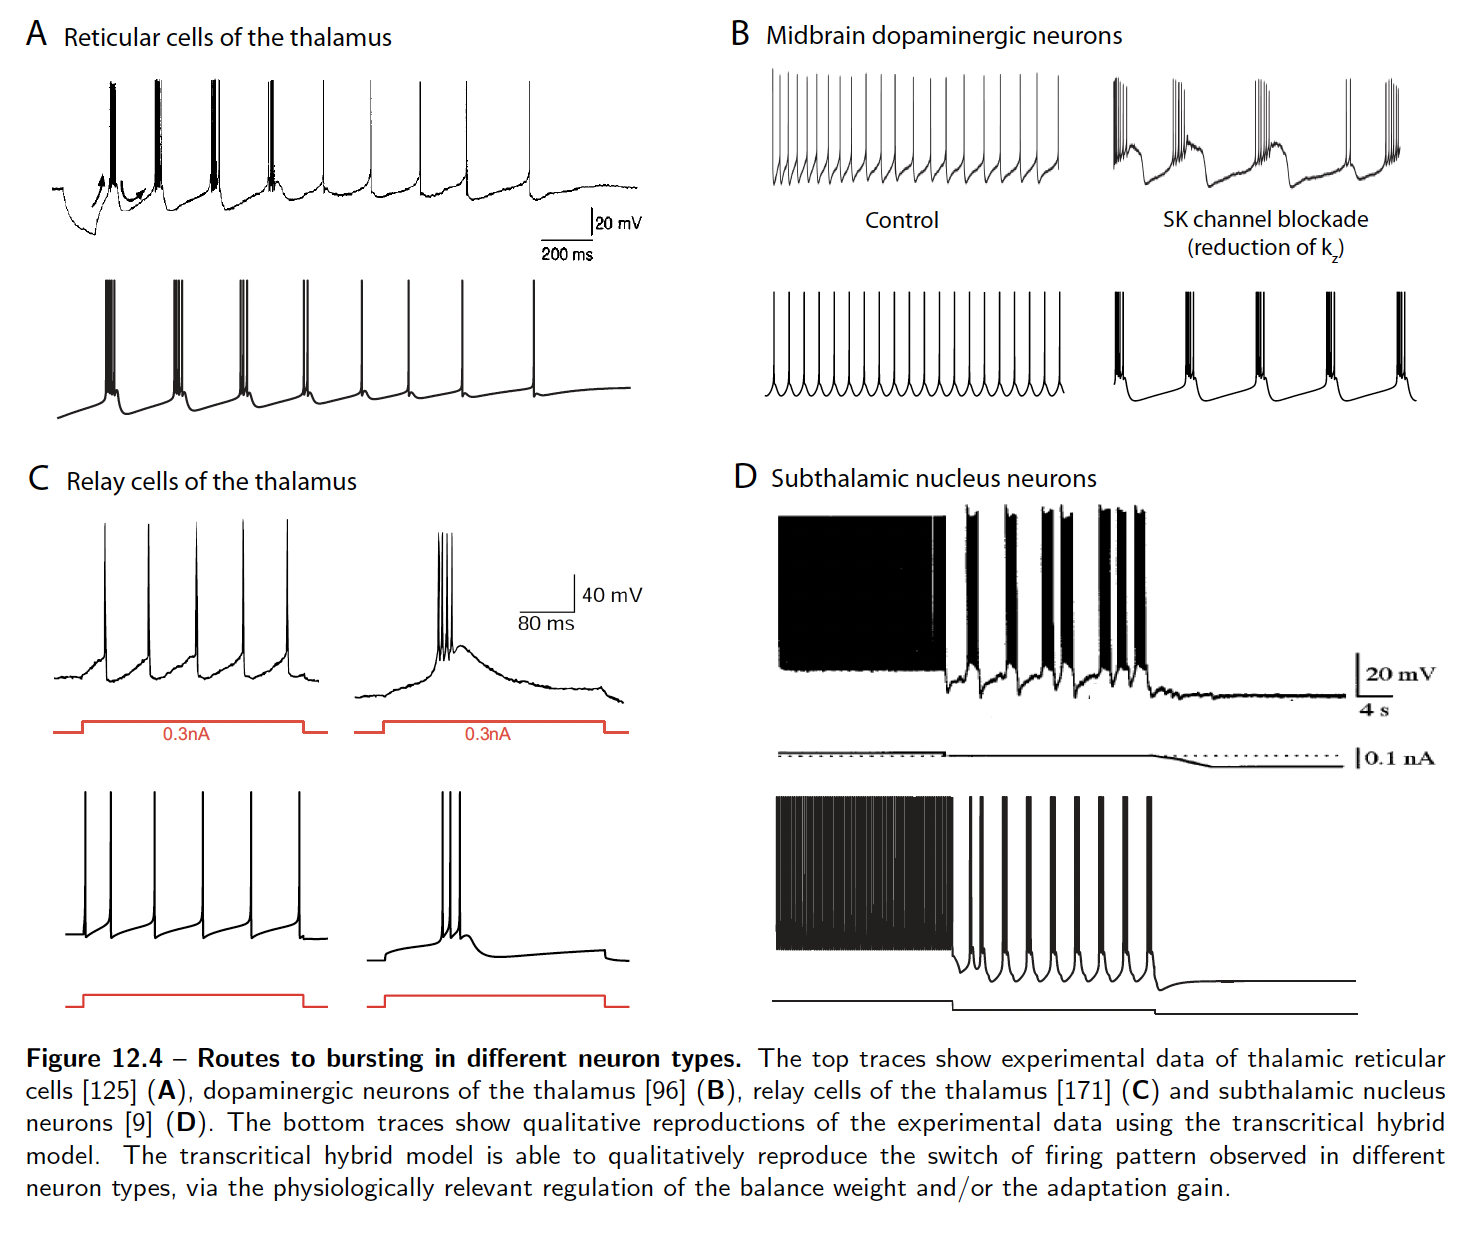
\includegraphics[scale=0.4]{latex/fig/Methods/GD_Thesis_Bursting.png}
    \caption{ ....}
    \label{fig:GD_Thesis_Bursting}
\end{figure}
\color{black}
\end{comment}


\color{black}
\subsection{The neuron model implemented in the context of this thesis}

\textcolor{red}{montrer une simu du modèle qui switch}

% -------------------------------
% -------------------------------
%
%     Circuit
%
% -------------------------------
% -------------------------------

\section{Circuit and network architecture}
Connecting neurons with each other is very easy following the electrical circuit equivalence of the neuron. Synaptic currents are simply modelled as input current:
$$ C_\mathrm{m}\dot{V}_\mathrm{m} = -\sum_i I_{\mathrm{ion},i} + I_{\mathrm{app}} + I_{\mathrm{syn}}.$$ 

In this thesis we consider four synaptic currents due to different postsynaptic receptors: \acrshort{AMPA}, \acrshort{GABA}\textsubscript{A} and \acrshort{GABA}\textsubscript{B}.

There are different manners to describe synaptic currents (see \citep{destexhe_circuit_2004}). In my thesis, I follow the \acrshort{HH} formalism such that the postsynaptic receptors allow flow of ions following the gradient concentration when the channel gate is open. The synaptic currents are defined by:
\begin{align*}
    I_{\mathrm{AMPA}}	&  = \bar{g}_{\mathrm{AMPA}} s_\mathrm{AMPA}(V_\mathrm{m} - 0) \\
    I_{\mathrm{GABA}_\mathrm{A}} &  = \bar{g}_{\mathrm{GABA}_\mathrm{A}}  s_{\mathrm{GABA}_\mathrm{A}} (V_\mathrm{m}-E_\mathrm{Cl})\\
    I_{\mathrm{GABA}_\mathrm{B}}   &= \bar{g}_{\mathrm{GABA}_\mathrm{B}} s_{\mathrm{GABA}_\mathrm{B}} (V_\mathrm{m}-E_\mathrm{K})
\end{align*}
where $\bar{g}_{\mathrm{AMPA}}$,  $\bar{g}_{\mathrm{GABA}_\mathrm{A}}$ and $\bar{g}_{\mathrm{GABA}_\mathrm{B}}$ are the synaptic conductances. \\
~\\
\textcolor{magenta}{ATTENTION ETRE COHERENT DANS la rédaction du mécanisme de plasticité et des notations. Latter $\bar{g}_{\mathrm{AMPA}}$ is multiplied by the synaptic weight $w$ (see Plasticity implementation).}


AMPA receptor reversal potential is set to \SI{0}{\milli\volt}, GABA\textsubscript{A} receptor reversal potential is set to chloride reversal potential ($E_\mathrm{Cl} = \SI{-70}{\milli\volt}$) and GABA\textsubscript{B}  receptor reversal potential is set to potassium reversal potential ($E_\mathrm{K} = \SI{-85}{\milli\volt}$).

The gating variables of the synaptic receptors are $s_\mathrm{AMPA}$, $s_{\mathrm{GABA}_\mathrm{A}}$ and $s_{\mathrm{GABA}_\mathrm{B}}$ are variables whose dynamics depend on the activity of the presynaptic neuron. As the presynaptic neuron spikes, it releases neurotransmitters that bind to the receptors and open the receptors. To shortcup all the biological reactions, the gating variable dynamics is simply governed by the presynaptic activity. In my thesis, I use the presynaptic membrane potential:
\begin{align*}
	\dot{s}_\mathrm{AMPA} & = 1.1 \, T_\mathrm{m} (1-s_\mathrm{AMPA}) - 0.19 \,s_\mathrm{AMPA} \\
	\dot{s}_{\mathrm{GABA}_\mathrm{A}} &= 0.53 \, T_\mathrm{m} (1- s_{\mathrm{GABA}_\mathrm{A}}) - 0.18 \,s_{\mathrm{GABA}_\mathrm{A}} \\
	\dot{s}_{\mathrm{GABA}_\mathrm{B}} &= 0.016 \, T_\mathrm{m} (1- s_{\mathrm{GABA}_\mathrm{B}}) - 0.0047\, s_{\mathrm{GABA}_\mathrm{B}}
\end{align*}
with transmitter concentration $T_\mathrm{m}$ depends on the presynaptic membrane voltage and the dynamics follows the formalism described in \cite{destexhe_synthesis_1994}, that is,
$$T_\mathrm{m}(V) = \dfrac{1}{1+\exp\left[-(V-2)/5\right]}.$$ 
The numerical values (1.1, 0.19, 0.53, 0.18, 0.016 and 0.0047) are rate parameters to mimic the kinetics of the synaptic receptors. These values originated from \cite{destexhe_synthesis_1994}. The smallest, the slowest the kinetics. For GABA\textsubscript{B}, the kinetics is slower which is coherent with the metabotropic nature of this receptor. Other models of synaptic receptor gating variables use the presynaptic spike time is integrated over time \textcolor{red}{REF}.

The synaptic current through \acrshort{NMDAr} requires an additional term modeling the effect of the magnesium blocker: 
$$ I_{\mathrm{NMDA}}	= \bar{g}_{\mathrm{NMDA}} B(V_\mathrm{m}) s_\mathrm{AMPA}(V_\mathrm{m} - 0) $$
where $B(V_\mathrm{m})$ is a sigmoidal function dependent on the postsynaptic membrane potential. For the purpose of this thesis, I follow the implementation of \citep{graupner_calcium-based_2012} to ease the implementation of synaptic plasticity \textcolor{red}{SEE SECTION}. 


\textcolor{blue}{jutifier le choix du réseau:} \citep{sherman_functional_1996}.\\

\textcolor{red}{expliquer que les courants synaptiques ne vont pas seulement utiliser V mais peuvent aussi utiliser les spikes times etc voir Destexhe 2004}


\subsection{Circuit used in the context of this thesis}
\textcolor{red}{montrer une simu d'un petit circuit à trois neurones}

~\\
\newpage

% -------------------------------
% -------------------------------
%
%            PLASTICITY
%
% -------------------------------
% -------------------------------

\section{Synaptic plasticity}
As described in the previous chapter, neurons have the ability to change their connections with each other based on their activities. Modeling synaptic plasticity consists in creating a model seen as a black box, that uses the pre- and postsynaptic activities as inputs and provided the synaptic strength as output. It is a challenging task because it requires several model decisions, called model features,  such as the choice of the region of interest, the network size, the neuron model and the definition of the synaptic strength. Then, the core of the challenge is to create the dynamics that governs the evolution of the synaptic strength, namely the synaptic plasticity rule itself. 

\textcolor{magenta}{etre rigoureuse dans la def de w partout}
%In the following section, I explain the diverse computational model features often encountered in the literature. 


\begin{figure}[h!]
    \centering
    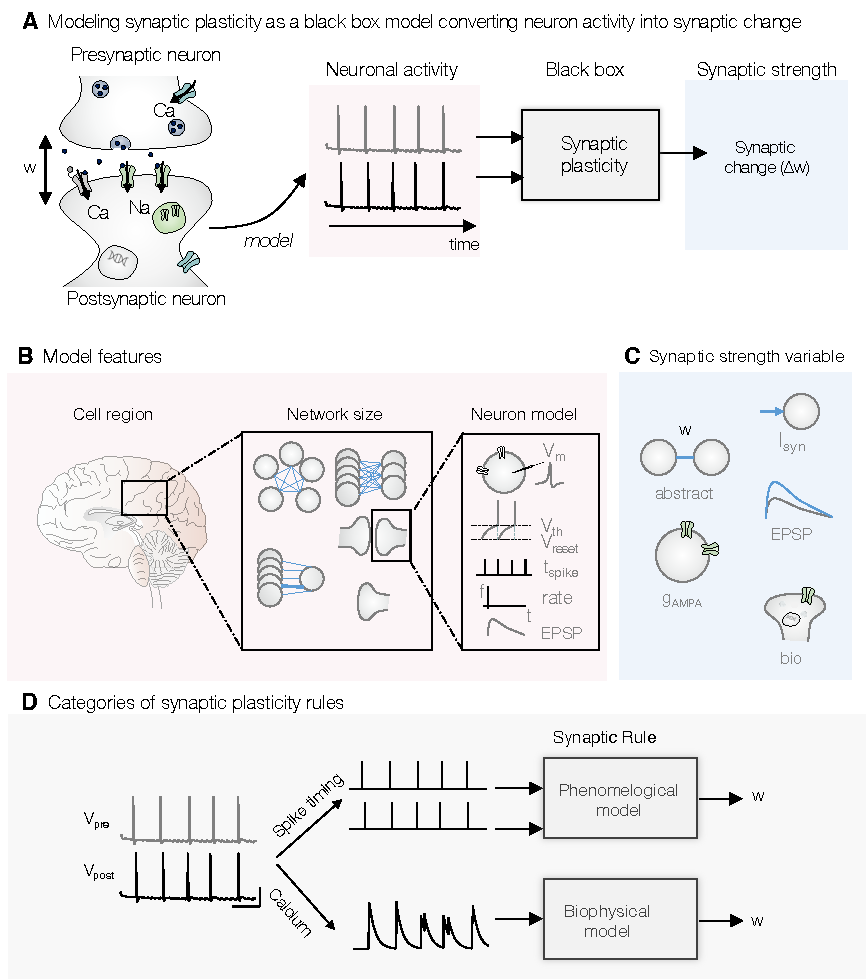
\includegraphics[scale=1]{fig/Methods/FeaturesRecap.pdf}
    \caption{Cpation}
    \label{fig:Methods_FeaturesRacap}
\end{figure}

\begin{comment}
    OLD CAPTION

    \caption{\textbf{A.} \textbf{Model features shared in computational models of synaptic plasticity rule}. \textit{Cell region}: plasticity can be explored in different neuron types located such as hippocampus, cortex, striatum or thalamus. The neuron parameters can be adapted to mimic different neuron types or one can use an abstract neuron. \textit{Network size}: plasticity can be studied in a network composed of several neurons or formed in assembly shape, between several presynaptic neurons projecting to one postsynaptic neuron, between a pre- and post-synaptic neuron or at the postsynaptic level. \textit{Neuron model}: the neuron follows a conductance-based model (with a membrane voltage Vm) or an \acrfull{IF} formalism. Only the spike trains or the firing rate is considered, or another principle is used such as the \acrshort{EPSP} or more complex neuron shape. \textit{Synaptic strength}: the weight is abstract and does not influence the rest (w, top-left scheme), the weight directly influences the synaptic input, the change in synaptic transmission is quantified by the change in \acrshort{EPSP} (top-right scheme), the change of \acrshort{AMPAr} is measured (bottom-left scheme) or the weight is measured by more biological quantities (bottom-right scheme).\\
    \textbf{B.} The synaptic weight $w$ change is governed by the neuronal activity thanks to phenomenological models (top) (written as phenom.) or by calcium thanks to biological models (bottom). \textcolor{red}{ajuster les couleurs avec les couleurs du rappel}}
    
\end{comment}

% -----------------------------------
%
%             SP (features)
%
% -----------------------------------

\subsection{Model features}
%Figure \ref{fig:Review_blackbox}A 
Table \textcolor{red}{XXX} gathers the different network and neuron features. 

% -----------------------------------
%       SP (features): neurons modeling choice
% -----------------------------------
\subsubsection{The region of interest}
First of all, synaptic plasticity varies depending on the brain \textit{region}. It has been commonly modeled for neurons in the hippocampus \citep{abarbanel_biophysical_2003, van_rossum_stable_2000}, the cortex \citep{chen_heterosynaptic_2013}, the striatum \citep{nakano_kinetic_2010, jedrzejewska-szmek_calcium_2017} or the thalamus \citep{gjorgjieva_burst-time-dependent_2009}. But thanks the freedom in computational models, a neuron can be adaptable by changing its parameters as done in \citep{graupner_calcium-based_2012, clopath_connectivity_2010} or we can encounter the notion of 'abstract neuron' meaning that the region or the type is not accurately defined and the parameters have been not fitted on experimental data. It is useful to study more general phenomenons or to study plasticity using the spike train only for example \citep{karmarkar_model_2002, liu_effects_2015} (it is correlated with the feature neuron modeling). 

% -----------------------------------
%       SP (features): network size
% -----------------------------------
\subsubsection{The network size}
The second feature is the \textit{network size}. Plasticity can be studied locally by considering only the postsynaptic site \citep{graupner_calcium-based_2012} or at the interconnection between a pre- and a postsynaptic neuron [...]. It is also common to see a large amount of presynaptic neurons projecting to a postsynaptic neuron \citep{chen_heterosynaptic_2013, gonzalez-rueda_activity-dependent_2018}. Thanks to the computer efficiency improvement, the network size can be increased from small networks of 10 neurons to very large network of thousands neurons [...]. Finally, memory engrams rise interest and can be studied in interconnected network \citep{delamare_intrinsic_2022}.




% -----------------------------------
%       SP (features): neurons modeling choice
% -----------------------------------
\subsubsection{Neuron modeling}
The third important feature is the computational model of the neuron, which must accurately reproduce its electrical activity. The most commonly used models include the \textit{conductance-based model (cond)}   \citep{hartley_understanding_2006, gerkin_phenomenological_2010}, the \textit{integrate-and-fire (IF)} model and its derivatives \citep{bush_calcium_2012, izhikevich_solving_2007}, the \textit{event-based} model   (event)\citep{shouval_converging_2002}, and \textit{rate-based} (rate) models \citep{delamare_intrinsic_2022}. More complex implementations, such as the description of the \acrfull{BPAP} and the \acrfull{EPSP}, have been developed, among others \citep{kumar_frequency-dependent_2011}. Although there are many other computational models of neuron activity, I will limit the discussion to these five approaches (as defined in \textcolor{red}{SECTION XXX}. For further information, refer to \citep{gerstner_neuronal_2014}.



% -----------------------------------
%       SP: calcium modeling
% -----------------------------------
\subsubsection{Calcium modeling}
 Calcium is often used as the key driver to induce synaptic change. The correspondence between the change in calcium and the related pre- and postsynaptic spiking is implemented in several manners. Here, I list some common modeling practices (see Table \ref{tab:calcium features}). First, the \textit{calcium source} must be explicit such as NMDAr or voltage dependent calcium channels (VDCC) [..]. It can also come from more complex mechanisms such as intracellular stores such as endoplasmic reticulum \citep{berridge_neuronal_1998, jaeger_spike_2014}. Calcium is also released via activation of metabotropic glutamate receptors. Others calcium-dependent mechanisms can be integrated such as calcium-extrusion mechanisms, including membrane pumps, intake and uptake into intracellular calcium-stores. Or by contrast, calcium can be abstract and explicitly described by a mathematical variable directly translating the neuronal activity without intermediate terms [...].  Second, calcium from NMDAr is frequently used, the \textit{description of NMDAr} is also various. It can be expressed by a simple synaptic variable equation [...], a more complex detailed equations of its kinetics [...] or relatively simple by converting the spike timing activity \citep{jaeger_spike_2014}. Finally, the \textit{calcium dynamics} provides the time-evolution of the calcium that is affecting the synaptic strength. Several descriptions exist. For example, a differential equation converts the calcium from NMDAr or NMDAr and VDCC into a calcium fluctuation [...]. Once again, its dynamics can be also expressed very abstractly [...] or with a lot of intermediate terms to mimic the whole complex process [...].


Table \ref{tab:calcium features} provides the overview of the different calcium modeling practices. Conceptual equations are presented. Each article might adapt the equation form for example by adding scaling factors. 
\\


\begin{table}[H]
\begin{small}
    \centering
    %\resizebox{\textwidth}{!}{%
    \begin{tabular}{lll}
    \hline
    Feature & Notation & Description \\
    \hline
    Calcium source     &  &\\
        &  $ I_{\mathrm{NMDA}}$ & 
        \begin{tabular}[l]{@{}l@{}}
        $I_{\mathrm{NMDA}} = g_{\mathrm{NMDA}} s_{\mathrm{NMDA}} B(V_{\mathrm{post}}) (V_{\mathrm{post}} - E_{\mathrm{NMDA}})$ \\ 
        $g_{\mathrm{NMDA}}$: NMDA conductance\\
        $s_{\mathrm{NMDA}}$: gating variable \\
        $B(V_{\mathrm{post}})$ :  ... \end{tabular}\\
        &  $ I_{\mathrm{NMDA}} + I_{\mathrm{VDCC}} $ & ...\\
        & Others & eg: buffers, diffusion terms, pumps, ... \\
        &  $ \mbox{NMDA}(t_{\mathrm{spk}}) $ & Decreasing exponential at each postsynaptic spikes. \\
    \hline
    NMDA model   &   & \\  
        & Time   & Pre- or postsynaptic spike times govern the NMDA equation \\
        & Voltage & Pre- and postsynaptic voltages govern the NMDA equation \\
        & Kinetics & NMDAr is described by kinetic equations \\
        & / & No biological current\\
        & Others & More complex process describe the NMDAr \\
    \hline
    Calcium dynamics & &  \\
        & NMDA & 
        \begin{tabular}[l]{@{}l@{}}
        $\tau_{\mathrm{Ca}} \dot{\mathrm{Ca}} = \alpha I_{\mathrm{NMDA}} - \mathrm{Ca}$ \\
        $\alpha$: current-to-concentration factor
        \end{tabular} \\
        & NMDA + VDCC & \begin{tabular}[l]{@{}l@{}}
        $\tau_{\mathrm{Ca}} \dot{\mathrm{Ca}} = (\alpha I_{\mathrm{NMDA}} + \beta I_{\mathrm{VDCC}}) - \mathrm{Ca}$ \\
        $\alpha, \beta$: current-to-concentration factors
        \end{tabular}\\
        & $\delta (t_{\mathrm{spk}})$ & Simplified equation converting spike times into calcium variation\\
        & Others / Process & More biophysical description of the calcium change  \\
    \hline
    \end{tabular}
    %}
    \end{small}
    \caption{\textbf{Model features used to implement calcium in a neuron model}. There are various sources of calcium that can be considered. The implementation of the NMDA receptor dynamics varies between model. Calcium dynamics can be governed by calcium current sources or more abstract translating spike time activity. \textcolor{red}{Décider si on explique les équations dans le tableau ou non ? } }
    \label{tab:calcium features}
\end{table}


% -----------------------------------
%       SP: definition in models
% -----------------------------------
\subsubsection{The definition of the synaptic strength}
The last feature is the \textit{definition of the synaptic strength $w$} (see Figure~\ref{fig:Methods_FeaturesRacap}C) . I highlight five widespread forms. 
\begin{itemize}
\item \textcolor{blue}{Abstract}\\
The weight $w$ is simply a variable updated by the synaptic plasticity rule and it is not interfering in other model equations. It is encountered in more theoretical papers. I call it an abstract definition \textcolor{red}{REF}. 
\item \textcolor{blue}{$I_{syn}$}\\
The term $w$ is present in the model and weights the synaptic input. In an Integrate-and-Fire model or in a conductance based model,  the synaptic current is written $I_{\mathrm{syn}} = w F_{\mathrm{syn}}$ where $F_{\mathrm{syn}}$ either a function of the spiking time $\delta(t_{\mathrm{spk}})$ or pre- or postsynaptic membrane voltage $I_{\mathrm{syn}} = \bar{g}_{\mathrm{syn}}(V-E_{\mathrm{syn}}) $ such as  $\bar{g}_\mathrm{syn} = w \bar{g}_{syn}$ (resp. $w \bar{g}_{\mathrm{AMPA}}, w \bar{g}_{\mathrm{NMDA}}$). In more mathematical models, it weights the synaptic activity as done in \citep{tetzlaff_synaptic_2013}.
\item \textcolor{blue}{$g_{AMPA}$}\\ 
The synaptic strength directly refers to the conductance of the AMPA receptors. It translated the increase in efficacy or number of AMPA receptors. The differential equation governing the conductance change is driven by the activity of pre- and post-synaptic neurons ($A_{\mathrm{pre}}$ and $A_{\mathrm{post}}$) \citep{berridge_calcium_2014}:
\[ \dot{g}_\mathrm{AMPA} = F(A_{\mathrm{pre}}, A_{\mathrm{post}})\]
\item \textcolor{blue}{Bio}\\
The strength is quantified by biological quantities, for example the change in the concentration of phosphorylated \acrshort{CaMKII} or the concentration of active and phosphorylated AMPAr \textcolor{red}{REF}.
\item \textcolor{blue}{EPSP}\\
As done in experiment, the change in synaptic strength is measured by the change in the \acrshort{EPSP} before and after the induction protocol.
\end{itemize}




% -----------------------------------
%       SP: black box
% -----------------------------------
\subsection{Traditional synaptic plasticity rules}
Modeling of synaptic plasticity
%, neuronal activity and neuromodulation 
is trendy these recent years. Browsing the literature to find a synaptic rule adapted to your research can be very challenging. The number of publications providing models of synaptic rules is increasing with years. The rules can be declined following a very abstract equation to a huge set of detailed plasticity signaling reactions. A myriad of reviews detail models of synaptic plasticity rules since the last 20 years \citep{morrison_phenomenological_2008, citri_synaptic_2008, feldman_spike-timing_2012, feldman_spike_2020, shouval_models_2007, sjostrom_spike-timing_2010, manninen_postsynaptic_2010, lisman_questions_2010, markram_history_2011, markram_spike-timing-dependent_2012, van_rossum_computational_2013, fusi_limits_2007, senn_spike-timing-dependent_2020, magee_synaptic_2020, chrol-cannon_computational_2014}. In the following section, I recall the notion of synaptic plasticity rule and I explain the most encountered models.


\begin{comment}
\begin{figure}[H]
    \centering
    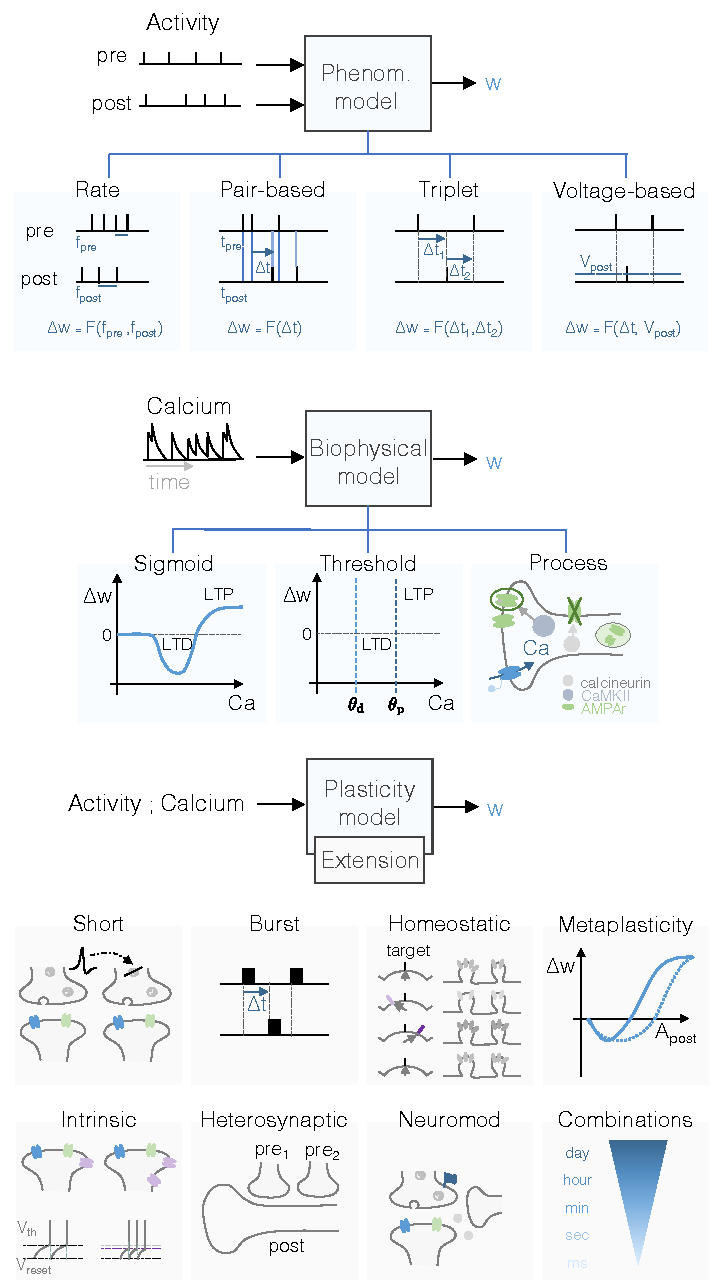
\includegraphics{fig/Review/ModelRecap.pdf}
    \caption{\textbf{Taxonomy of synaptic plasticity rules} . (Top) Phenomenological synaptic plasticity rules compute the synaptic weight change from the pre and post synaptic activities. Four main models are implemented: rate [...], pair-based [...], triplet [...] and voltage-based [...]. (Center) Biophysical models use the calcium signal that drives the synaptic weight change. Three main models exist: sigmoid \citep{shouval_unified_2002}, threshold \citep{graupner_calcium-based_2012} and process encapsulated more complex models [..]. (Bottom) Several extension rules are often encountered: short-term plasticity (short), burst-time dependent plasticity (burst), homeostatic plasticity, metaplasticity, intrinsic plasticity, heterosynaptic plasticity, neuromodulated-plasticity rule (neuromod), combinations of diverse rules. }
    \label{fig:ModelRecap}
\end{figure}
\end{comment}


\subsubsection{Categories of synaptic plasticity rules}
Once the region, the network, the neuron and the definition of the synaptic strength have been established, the next primordial step is the implementation of the synaptic plasticity rule. It is translated by an equation describing the evolution of the weight $w$ throughout time $\dot{w}$. The synaptic rule can be seen as the \textit{black box} converting pre and postsynaptic activity as input ($A_{\mathrm{pre}}$ and $A_{\mathrm{post}}$), which are implemented for example by the spike times, the firing frequency of the pre- and postsynaptic neurons or the calcium concentration and providing the synaptic change as output (see Figure~\ref{fig:Methods_FeaturesRacap}A)  The generic equation is:
$$ \dot{w} = F(A_{\mathrm{pre}}, A_{\mathrm{post}})$$
\textcolor{orange}{(see Figure \ref{fig:blackbox}B)}\\

~\\
Two main categories of synaptic rules are distinguished \citep{shouval_models_2007, graupner_synaptic_2017, clopath_long-term_2019}(see Figure~\ref{fig:Methods_FeaturesRacap}D): 
\begin{itemize}
    \item \textit{Phenomenological models} estimate the synaptic strength change by translating the relationship between neuronal activity and the synaptic plasticity. This category of model expressed mathematically the relation between the pre- and post spike times $(t_{\mathrm{pre}}, t_{\mathrm{post}})$, the firing frequency $(f_{\mathrm{pre}}, f_{\mathrm{post}})$ or the neuronal activity  to estimate the change in synaptic strength. This approach focuses on abstract equations able to fit experimental data rather than describing all molecular processes underneath.
    \item \textit{Biophysical models} using biological variables to drive the induction and expression of synaptic plasticity such as calcium concentration or a cascade of kinase activation for example. Indeed, calcium is a good indicator of voltage, frequency, action potential variation \citep{feldman_spike-timing_2012}.
\end{itemize}

An overview of the most common encountered synaptic plasticity rules is shown in Figure \ref{fig:ModelRecap}. The following sections explained their implementations. This method of classification and model description was started in \citep{clopath_long-term_2019}. 


\subsubsection{Synaptic plasticity rule limitations}
In the context of this thesis, I am restricting my research on excitatory synaptic plasticity and I put aside the inhibitory synaptic plasticity. For more details, refer to \citep{wu_regulation_2022}. Models of plasticity in the field of machine learning and artificial intelligence such as backpropagation for example are out of scope. 

I am interested in articles that investigate the change in synaptic strength due to neuronal activity in order to understand learning, memory formation and memory consolidation. 


\subsubsection{Fitting the parameters of the black box on experimental data}
To create a model, one must choose values for various parameters. To parameterize a synaptic plasticity rule, a common practice is to replicate a plasticity-inducing protocol, as illustrated in Figure \ref{fig:SP_Protocols}. The goal is to fit the experimental points, the two most often encountered dataset is the \acrshort{STDP} provided by \citep{bi_synaptic_1998} (see Figure~\ref{fig:SP_STDP}) or the frequency-dependent plasticity protocol provided by \citep{sjostrom_rate_2001}.


\subsubsection{Phenomenological models}
In phenomenological models, four pioneered synaptic rules were established in the last 20 years: Rate-based, pair-based, triplet and voltage-based as illustrated in Figure \ref{fig:ModelRecap} (top) \citep{gerstner_hebbian_2011, feldman_spike-timing_2012,  feldman_spike_2020}.



In line with the Hebbian principle \citep{hebb_organization_1949}, first models of synaptic plasticity consider only the \textit{rate} of pre- and postsynaptic neurons ($f_{\mathrm{pre}}$, $f_{\mathrm{post}}$) to determine the sign and magnitude of plasticity  [\textcolor{blue}{model:}\cite{oja_simplified_1982, bienenstock_theory_1982, udakis_interneuron-specific_2020}. The \textit{Pair-based} model often called the \textit{\acrfull{STDP}}
[\textcolor{blue}{review}: \cite{abbott_synaptic_2000,morrison_phenomenological_2008})] suggests the equation to fit the experimental data resulting from the plasticity-induction protocol \citep{bi_synaptic_1998}. The pre and the postsynaptic neurons are spiking at  given frequency and the synaptic change depends on the spiking time lag $\Delta t$. It is used in several studies since 20 years [\textcolor{blue}{model}: \cite{van_rossum_stable_2000,song_competitive_2000, capone_sleep-like_2019}. The classical depression-potentiation kernel has been shown to change depending on the region or the animal [\textcolor{blue}{review}: \cite{abbott_synaptic_2000}. It has been exploited for example in \citep{liu_effects_2015} A comprehensive history of STDP is established in [\textcolor{blue}{review}: \cite{markram_history_2011, feldman_spike_2020}. This rule is constrained by some limitations \citep{babadi_stability_2016}. The \textit{triplet} rule considers the effect of spike triplets such as pre-post-pre or post-pre-post [\textcolor{blue}{model}: \cite{froemke_spike-timing-dependent_2002, pfister_triplets_2006, costa_unified_2015, gjorgjieva_triplet_2011}. \textit{Voltage-based} rules take into account the spike-timing in pre- and postsynaptic neurons as well as the membrane voltage of the postsynaptic neurons [\textcolor{blue}{model}: \cite{brader_learning_2007, clopath_connectivity_2010} in order to reproduce a larger variety of experimental protocols \citep{sjostrom_rate_2001, artola_different_1990, nevian_spine_2006}. 
~\\




\begin{figure}[h!]
    \centering
    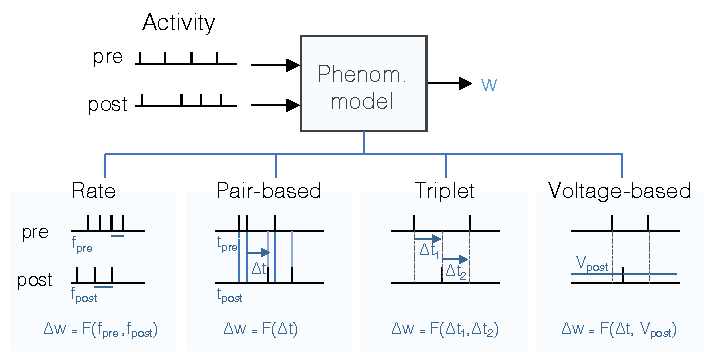
\includegraphics{latex/fig/Methods/ModelRecap_Phenom.pdf}
    \caption{Caption}
    \label{fig:my_label}
\end{figure}


\subsubsection{Calcium-based models}
This part of the review only covers computational models using calcium as the key driver of the synaptic rule. These rules provide equations explaining the calcium influx dependency. Either kinase or phosphatase proteins are activated leading to an increase or decrease of the strength \citep{meriney_synaptic_2019}. This phenomenon is implemented into the synaptic rule with different levels of complexity depending on the model. I highlight three pioneered rules (see Figure \ref{fig:ModelRecap}(center): sigmoid, threshold, and process. 

First, the synaptic change is governed by a \textit{sigmoid} function of the calcium level: $
\tau_w([\mathrm{Ca}]) \dot{w} = \mbox{sig}([\mathrm{Ca}]) - [\mathrm{Ca}] $. It accounts for low calcium level does not change the synaptic weight (or at a extremely slow timescale). Intermediate level triggers slow depression while high calcium level triggers fast potentiation. It reproduces the phosphatase and kinase action. This rule was pioneered by the calcium control hypothesis from \citep{shouval_unified_2002}. The governing rule was further developed throughout time [\textcolor{blue}{model:} \cite{ karmarkar_model_2002, kumar_frequency-dependent_2011, shouval_stochastic_2005, shah_biophysical_2006,cai_effect_2007, carlson_interplay_2011, rackham_ca2-based_2010}. It was used in several applications such as task orientation in place cells or to investigate the effect the dendritic properties
[\textcolor{blue}{model:} \cite{yu_biophysical_2008, iannella_nonlinear_2014, odonnel_dendritic_2011, franks_complexity_2002}. The comparison with phenomeological models such as pair-based on triplet is established in \citep{shouval_what_2011}.


Then, the sigmoid function describing the continuous relationship between calcium concentration and synaptic change was simplified by \citep{graupner_calcium-based_2012} into a two-\textit{thresholds} calcium levels triggering depression and potentiation. The governing expression is $ \tau_w \dot{w} = \gamma_\mathrm{p}(1-w) \Theta([\mathrm{Ca}]-\theta_\mathrm{p}) - \gamma_\mathrm{d} w \Theta([\mathrm{Ca}]-\theta_\mathrm{d})$ where $\tau_w$ is the time constant associated to synaptic change, $\gamma_p$ and  $\gamma_\mathrm{d}$ are respectively the potentiation and the depression rates, $\Theta([\mathrm{Ca}]-\theta_\mathrm{p})$ means $\Theta = 1$ if $[\mathrm{Ca}]>\theta_\mathrm{p}$ otherwise $\Theta = 0$. The comparison with phenomenological models is established in \citep{graupner_natural_2016}. It was used in several studies for various regions such as cerebellum or striatum and diverse applications such as memory formation in large-scale network, \textcolor{blue}{model:} \citep{bouvier_burst-dependent_2016, chindemi_calcium-based_2020, olcese_sleep_2010, standage_calcium-dependent_2014, higgins_memory_2014, inglebert_synaptic_2021, deperrois_short-term_2020,lappalainen_theoretical_2019,jedrzejewska-szmek_calcium_2017}.

A third approach uses intermediate steps that first convert calcium influx into intermediate signals and the change in these signals affect the synaptic weight such as $\dot{w} = F(P),  \dot{P} =F([\mathrm{Ca}])$ where  $P$ quantifies phosphorylation and dephosphorylation processes [\textcolor{blue}{model:} \citep{abarbanel_biophysical_2003, rubin_calcium_2005, badoual_biophysical_2006, hartley_understanding_2006, graupner_stdp_2007, gerkin_phenomenological_2010, bush_calcium_2012, houben_calcium-influx-dependent_2020, kornijcuk_simplified_2020, saudargiene_inhibitory_2015, ebner_unifying_2019}. The level of details in calcium-driven varies a lot and it helps to provide a degree of freedom to explore the effect of biological factors, for example, the contribution of endoplasmic reticulum  \textcolor{blue}{model:} \citep{ kubota_model_2008, urakubo_requirement_2008, mahajan_intracellular_2019}.


This review limits its investigation for articles that are only using a small amount of intermediate signals and excludes papers proposing  detailed mechanisms of the effect of calcium influx on the strength by more intermediates, for example an interesting model is presented in \cite{maki-marttunen_unified_2020, kotaleski_modelling_2010}. Other reviews like \cite{graupner_mechanisms_2010, jaeger_spike_2014} further examine and compare, calcium data, models depending only on calcium concentration, or implement biochemical signaling cascades beyond calcium. 



\begin{figure}[h!]
    \centering
    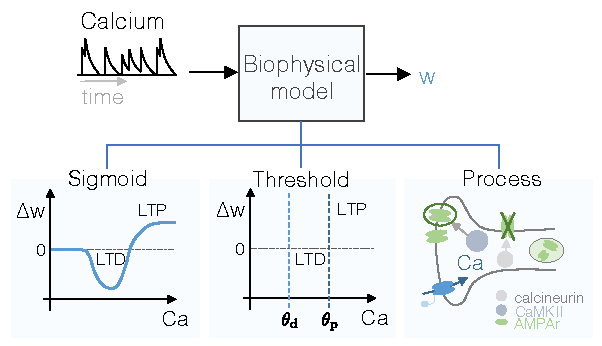
\includegraphics{latex/fig/Methods/ModelRecap_Ca.pdf}
    \caption{Caption}
    \label{fig:my_label}
\end{figure}

\begin{table}[H]
\centering
\begin{small}
\resizebox{\textwidth}{!}{%
\begin{tabular}{llll}
\hline
    Model & Equation &  & Reference  \\
\hline
\multicolumn{4}{c}{\textbf{Phenomenological models}}  \\ 
\hline
    Rate-based & $\dot{w} = F(f_{\mathrm{pre}}, f_{\mathrm{post}})$  &  & \cite{bienenstock_theory_1982}\\
    & & & \cite{oja_simplified_1982}\\
    Pair-based & $\dot{w} = F(\Delta t)=\left\{\begin{array}{ll}A^{+} \exp \left(-\Delta t / \tau^{+}\right) & \Delta t>0 \\- A^{-} \exp (\Delta t / \tau^{-}) & \Delta t<0\end{array}\right.$  &  & \cite{song_competitive_2000}\\
    & & & \cite{van_rossum_stable_2000}\\
    Triplet &  $\dot{w} = F(\Delta t_1, \Delta t_2)$ &   & \cite{pfister_triplets_2006} \\
    Voltage-based & $\dot{w} = F(\Delta t, V_{\mathrm{post}})$ & & \cite{clopath_connectivity_2010}\\
\hline
\multicolumn{4}{c}{\textbf{Biophysical models}}  \\ 
\hline
    Sigmoid   & $\tau_w([\mathrm{Ca}]) \dot{w} = \mathrm{sig}([\mathrm{Ca}]) - [\mathrm{Ca}]$   &  & \cite{shouval_unified_2002} \\
    Threshold &  & & \cite{graupner_calcium-based_2012} \\
    & \begin{tabular}[l]{@{}l@{}} $[\mathrm{Ca}]< \theta_\mathrm{d} :  \dot{w}=0$\\ $\left[\mathrm{Ca} \right] \in \left[\theta_\mathrm{d}, \theta_\mathrm{p} \right] :  \dot{w}=\nearrow$ \\ $\left[\mathrm{Ca} \right] > \theta_\mathrm{p} :  \dot{w} \searrow$ \end{tabular} & & \\
    Process &  \begin{tabular}[l]{@{}l@{}}$\dot{w} = F(P)$ \\ $dP/dt = F([\mathrm{Ca}])$ \end{tabular} &  & \cite{abarbanel_biophysical_2003}\\
\hline
\end{tabular}
}
\end{small}
\caption{Overview of synaptic plasticity rule implementations for phenomenological models or biophysical models. Each category is decomposed into their pioneered rules. Conceptual equations for the synaptic change $\dot{w}$ is provided with a brief description. \textcolor{orange}{Questions: (1)  Ajouter les descriptions ou mettre en caption les symboles $\Delta t$ ? (2) est-ce qu'on cite plusieurs articles par règle ? par exemple pour process il y en a plusieurs ..}}
\label{tab:Phenom}
\end{table}



\subsubsection{Extended models}
The previous synaptic rules are well-known in the literature but it was shown that they cannot explain all the various complex synaptic processes. In this section, we present models describing complementary synaptic mechanisms: (i) short term plasticity, (ii) burst-dependent plasticity, (iii) homeostasis, (iv) metaplasticity, (v) intrinsic plasticity, (vi) heterosynaptic plasticity, (vii) neuromodulated-plasticity and (viii) combinations of synaptic rules. The overview of the extension models are shown in Figure \ref{fig:ModelRecap}(bottom). Table \ref{tab:extensions} briefly presents the implementation of these different extensions and their mechanisms. It extended the work presented in \citep{clopath_long-term_2019}. 

\begin{figure}[h!]
    \centering
    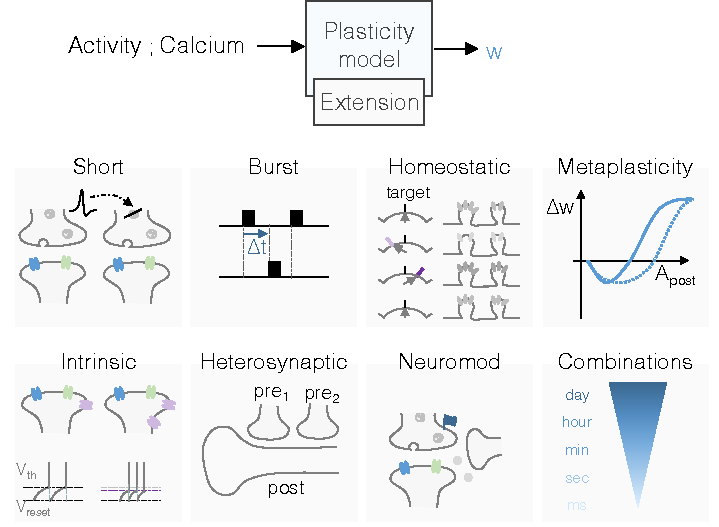
\includegraphics{latex/fig/Methods/ModelRecap_Extension.pdf}
    \caption{Caption}
    \label{fig:my_label}
\end{figure}






(i) \textit{\acrfull{STD}} explains that after an action potential, presynaptic resources such as vesicles transporting neurotransmitters are depleted and need to recover to their initial value before being able to act again [\textcolor{blue}{review/bio:} \cite{zucker_short-term_2002}. It is well known as the Markram-Tsodyks model [\textcolor{blue}{model:} \cite{markram_regulation_1997}. Nowadays, it is common to encountered synaptic plasticity rules including short-term depression in the model [\textcolor{blue}{model:} \cite{zenke_diverse_2015, chen_heterosynaptic_2013, olcese_sleep_2010, shah_biophysical_2006, cai_effect_2007, deperrois_short-term_2020, carvalho_novel_2011, hansel_short-term_2013}. \textcolor{red}{est-ce que je cite uniquement les papiers qui intègrent de la STD ou bien des papiers qui utilisent de la STD avec d'autres combinaisons de règles ? }\\

(ii) The \textit{\acrfull{BTDP}} focuses on the timing of pre- and postsynaptic bursts of activity instead of single-spikes as done in STDP. It permits to integrate the effect of high-frequency burst in the synaptic rule [\textcolor{blue}{model:} \cite{gjorgjieva_burst-time-dependent_2009, delattre_network-timing-dependent_2015, payeur_burst-dependent_2020}.\\


(iii)  Hebbian learning rule often leads to a runaway of synaptic strengths \citep{babadi_stability_2016}. Once the synaptic strengths are modified by a learning rule it can affect the neuronal activity. To counterbalance this problem,  \textit{homeostatic plasticity} refers to compensatory processes operating at various spatial and temporal scales \textit{allowing stabilization of neuronal activity}
[\textcolor{blue}{review:} \cite{turrigiano_homeostatic_2004, karabanov_consensus_2015, meriney_synaptic_2019,desai_homeostatic_2003}. More information on the biological explanations are given in \citep{shepherd_arcarg31_2006}. 

If the target neuronal activity is the firing rate: the concept of homeostatis stands that the connections between neurons should be either scaled up or down respectively as the firing rate decreases or increases [\textcolor{blue}{review} \cite{desai_homeostatic_2016}. In a modeling point of view, this \textit{synaptic scaling} or \textit{normalization} can be implemented via a multiplicative or substractive modifications of the synaptic weights
\citep{oja_simplified_1982}.  If the target neuronal activity is the intracellular calcium level to maintain homeostasis, [\textcolor{blue}{model:} \cite{oleary_cell_2014} developed an homeostatic rule regulating the synaptic conductances as well as the ion channel conductances (see later: intrinsic plasticity). In [\textcolor{blue}{model:} \cite{yeung_synaptic_2004}, the NMDA conductance is regulated leading to regulation of the calcium influx through the NMADr.   \\

(iv) \textit{Metaplasticity} is often called "plasticity of synaptic plasticity" and states that previous activity at the synapse can influence LTP or LTD  [\textcolor{blue}{review:} \cite{ abraham_metaplasticity_1996, abraham_metaplasticity_2008, abraham_is_2019,  meriney_synaptic_2019, deisseroth_synaptic_1995, yger_models_2015, lee_mechanisms_2019}. It can be seen as a modulation of the synaptic rule itself at a larger timescale. In [\textcolor{blue}{model:} \cite{zenke_synaptic_2013, benuskova_stdp_2007}, synaptic rule parameters vary as function of the moving firing rate. Metaplasticity was also investigated in calcium based models [\textcolor{blue}{model:} \cite{yu_biophysical_2008, anirudhan_analogous_2015}.

At this stage, the different terms can be confusing because metaplasticity can be homeostatic or not. If the metaplasticity is homeostatic; the synaptic rule changes itself with the aim of maintaining a target activity \citep{karabanov_consensus_2015}. Metaplasticity that is not homeostatic simply refers to a modification of the synaptic plasticity rule parameters. Similar reasoning, homeostasic plasticity is metaplasticity, if the rule changes or is not metaplastic if different parameters such as the weights are scaled or the intrinsic properties are perturbed. \\

(v) Until now, we have presented plasticity rules that affect the synaptic connection between neurons. However, activity-dependent modification of intrinsic neuronal excitability performed by change of neuronal membrane properties, more specifically  the number, distribution or activity of various ion channels located throughout the neuron  is another mode of memory formation and storage [\textcolor{blue}{review:} \cite{debanne_plasticity_2019, caverzasio_brain_2018, daoudal_long-term_2003, zhang_other_2003, oleary_computational_2015}.  This mode is called \textit{intrinsic plasticity} \citep{titley_toward_2017}. Two of the pioneered papers in this field are \citep{lemasson_activity-dependent_1993, liu_model_1998}.


Once again, intrinsic plasticity can be homeostatic as summarized in [\textcolor{blue}{review:} \cite{williams_homeostatic_2013, turrigiano_hebb_2000} and model in [\textcolor{blue}{model:} \cite{honnuraiah_calcium-dependent_2013, oleary_cell_2014}. Another implementation of intrinsic plasticity in a integrate-and-fire model is achieved by tuning regulating the firing threshold [\textcolor{blue}{model:} \cite{wu_homeostatic_2020}. In rate-based model, intrinsic plasticity tunes the excitability threshold [\textcolor{blue}{model:} \cite{delamare_intrinsic_2022}.  Homeostatic plasticity, intrinsic plasticity and metaplasticity can be hard to identify or separate in some models. The three concepts can be modeled based with concomitant rules. Likewise, one rule can support those concepts as shown in 
[\textcolor{blue}{model:} \cite{sehgal_learning_2013} where the intrinsic plasticity exhibits metaplasticity. \\


%Altogether, intrinsic plasticity and synaptic plasticity can be combined for the benefit of homeostatic regulation of neuronal excitability in order to maintain a target level of electrical activity. In a computational point of view, it can be seen as a controller where the target activity level is the reference such as a given frequency for phenomenological model or calcium level for calcium-based models see later. The intrinsic synaptic rule is the control rule itself transforming the input, ie the activity, into a modification of intrinsic property such as the ion-channel parameters.


(vi) The classical view of synaptic plasticity is built on both presynaptic and postsynaptic neuron activation for plasticity induction.  The rules previously described are input-specific and can be categorized as homosynaptic plasticity. However, at the same postsynaptic neuron, \textit{heterosynaptic plasticity} refers to changes at synapses that are not presynaptically active during the induction protocol, in others words, the synaptic change is induced by activity in neighboring synapses [\textcolor{blue}{review:} \cite{meriney_synaptic_2019, timofeev_sleep-wake_2019}.  Calcium in one synapse can trigger change in the neighboring synapses [\textcolor{blue}{review:} \cite{ bannon_homeostatic_2016, chistiakova_heterosynaptic_2014, froemke_plasticity_2015}. Thus, heterosynaptic plasticity is generated by the same protocols, operates at the same timescale and shares similar mechanisms with homosynaptic plasticity. It offers a solution for competition and stabilization by providing a rapid normalization of synaptic strength over individual cells and multi-cellular networks. In a computational point of view, the synaptic strength is driven as already explained by the pre- and postsynaptic neuronal activity as well as the neighboring activity (phenomenological manner) or by affecting modeling the calcium fluctuation coming from the pre, post and neighboring synapses (biophysical manner)  [\textcolor{blue}{model:} \cite{chen_heterosynaptic_2013, field_heterosynaptic_2020, hiratani_detailed_2017, li_induction_2016, fiete_spike-time-dependent_2010}. \\

(vii) Experimental studies have more recently investigated  the interaction of \textit{neuromodulation} and synaptic plasticity (see [ \textcolor{blue}{bio:} \cite{seol_neuromodulators_2007, zhang_gain_2009, salgado_noradrenergic_2012, pawlak_dopamine_2008, nadim_neuromodulation_2014}). The effect of the different neuromodulators on synaptic plasticity are very complex. To name a few, neuromodulatory inputs gate STDP rules via modification of neuronal excitability and spiking dynamics or alteration of intracellular signaling cascades implied in synaptic
plasticity [ \textcolor{blue}{review:} \cite{brzosko_neuromodulation_2019,fremaux_neuromodulated_2015, pawlak_timing_2010}. There are several ways to derive neuromodulated synaptic plasticity. The first one is inspired by neuromodulated-STDP. While adding neuromodulators during the STDP protocol, the kernel is shifted [\textcolor{blue}{model:} \cite{pedrosa_role_2017, gonzalez-rueda_activity-dependent_2018, izhikevich_solving_2007, legenstein_learning_2008}. Another technique relies on the creation of a mathematical framework called a "\textit{three-factor rule}". Plasticity is driven by the pre- and postsynaptic activity  as well as, a global factor seen as an extrinsic signal since it is not generated itself by the considered neurons but rather by others structures [\textcolor{blue}{review:} \cite{marder_neuromodulation_2012, fremaux_reinforcement_2013, izhikevich_solving_2007, brzosko_neuromodulation_2019, fremaux_neuromodulated_2015,schultz_behavioral_2006, foncelle_modulation_2018}. A synaptic \textit{eligibility trace} $e(t)$ bridges the temporal gap between the neural activity and the neuromodulatory signal. In experimental literature, this  eligibility trace is also called a 'tag'. It means that the synapse is 'tagged' and 'eligible' for change later on \citep{fremaux_neuromodulated_2015, magee_synaptic_2020}. But the synaptic change requires a modulatory signal to be effectively operated. One pays attention to the distinction between the two variables $w$ and $e$. The variable $w$ refers to the synaptic weight. The internal variable $e$ is not measurable in standard electrophysiological experiment \citep{gerstner_eligibility_2018}. More details on the mathematical implementation are available on \cite{izhikevich_solving_2007, legenstein_learning_2008,gerstner_eligibility_2018,fremaux_neuromodulated_2015, pawlak_timing_2010, madadi_asl_dopaminergic_2018}.  

This framework is attractive for reward-based learning, surprise-based learning and novelty-based learning in the sense that the tag exists on the timescale of seconds [\textcolor{blue}{model:} \cite{nakano_kinetic_2010, zannone_acetylcholine-modulated_2018, ang_functional_2021}. In addition, this mathematical formalism is used for memory consolidation and especially for sleep-dependent memory consolidation with the hypothesis called \textit{\acrfull{STD}} [\textcolor{blue}{review:} \cite{seibt_primed_2019}. Indeed, synapses are \textit{tagged} during learning phase and the neuronal network reactivation promotes the \textit{capture} and translation of Plasticity Related Products (PRPs) (including proteins or mRNA synthesis) to engage the pruning or weakening of the tagged synapses [\textcolor{blue}{model} \cite{luboeinski_memory_2021, ziegler_synaptic_2015, clopath_tag-trigger-consolidation_2008, clopath_synaptic_2012}. The website \url{https://www.science.gov/topicpages/r/reward-modulated+spike-timing-dependent+plasticity.html#} gathers numerous models of neuromodulated-synaptic plasticity rules. In brief, the three main modeling strategies of neuromodulated synaptic plasticity are: shifting the STDP kernel by mimicking neuromodulator effects, adding a third-factor term also called eligibility trace or implementing a STC plasticity rule.  \\


(viii) Synaptic plasticity is complex occurring at different places and at different timescales. It is likely that one rule alone is not enough to have the all picture of the different mechanisms. Therefore, several papers \textit{combine different synaptic rules} at different timescales such as STDP, short term plasticity, metaplasticity or homeostasis altogether [\textcolor{blue}{model:} \cite{honnuraiah_calcium-dependent_2013, bannon_adenosine_2017, fauth_self-organized_2019, zenke_diverse_2015, farries_reinforcement_2007, wu_homeostatic_2020,  el_boustani_stable_2012, nere_sleep-dependent_2013, vignoud_interplay_2018}.



\begin{table}[h!]
    \centering
    \resizebox{\textwidth}{!}{%
    \begin{tabular}{llll}
    \hline
    Rule & Equation  &  Description & Reference \\
    \hline
    Short-term &
    & & \cite{zucker_short-term_2002}  \\
    &$\tau_{ST} \dot{X}_{ST} =1-X_{ST}$   &  \begin{tabular}[l]{@{}l@{}} 
    $X_{ST}$: presynaptic resource, \\ $\tau_{ST}$: resource recovery time-constant  \end{tabular} & \cite{zenke_diverse_2015}\\
    \hline
    Burst & $\dot{w} = F(\Delta t^{\mathrm{burst}})$  & $ \Delta t^{\mathrm{burst}}$: relative pre and post synaptic burst timelag & \cite{gjorgjieva_burst-time-dependent_2009} \\
    \hline
    Homeostasis & & & \\
     & scaling: $w = w/w_{\mathrm{max}}$ & $w_{\mathrm{max}}$: maximum weight & \cite{turrigiano_homeostatic_2012} \\
     & target activity: $ \dot{x} \alpha A_{\mathrm{tgt}} - A $ & 
     \begin{tabular}[l]{@{}l@{}} 
     $x$ : weight or ionic conductance\\
     $A_{\mathrm{tgt}}$: target activity \\
    $A$: current activity  \end{tabular}
    & \cite{williams_homeostatic_2013}\\
    & & & \cite{desai_homeostatic_2016}\\
    \hline 
    Metaplasticity & 
    \begin{tabular}[l]{@{}l@{}} 
    $\tau_w \dot{w} = F(\theta)$\\
   $\tau_\theta \dot{\theta} = F(A_{\mathrm{post}})$
    \end{tabular}
    &
    \begin{tabular}[l]{@{}l@{}} 
    $\theta$: ...\\
   $A_{\mathrm{post}}$: ...
    \end{tabular}
    & \cite{abraham_metaplasticity_1996} \\
    \hline
    Intrinsic & \begin{tabular}[l]{@{}l@{}} $\dot{g}_{\mathrm{ion}} = F(A)$ \\ $g_{\mathrm{ion}}$: neuron-related variable \\
    (ion channel conductance, excitability,...)\\
    $A$: neuronal activity 
    \end{tabular} & & ... \\
    \hline
    Heterosynaptic & $\dot{w_{kj}} = F(A_i,A_j, A_k)$ &
    \begin{tabular}[l]{@{}l@{}}
    $A_{i,j}$: activity of presynaptic neuron i or j\\
    $A_{k}$: activity of postsynaptic neuron k\\    
    Activity is can be spike times or calcium concentration
    \end{tabular} &  \cite{chen_heterosynaptic_2013}\\
    & & & \cite{field_heterosynaptic_2020}\\
    \hline
    Neuromodulated & STDP kernel shift &
    & \cite{pedrosa_role_2017} \\
    &eligibility trace     &  & \cite{foncelle_modulation_2018}\\
    & STC   & & \cite{clopath_tag-trigger-consolidation_2008}\\
    & \begin{tabular}[l]{@{}l@{}}
    $\dot{w} = F(A_{\mathrm{pre}}, A_{\mathrm{post}}, M)$\\
    $M$: Neuromodulator variable
    \end{tabular}  & &\\
    \hline
    Combination & $\dot{w} = F(\mathrm{rule}_1, \mathrm{rule}_2)$ & Combinations of different synaptic rules at different timescales & \cite{zenke_diverse_2015}\\
    & & &\cite{fauth_self-organized_2019}\\
    & & & ... \\
    \hline
    \end{tabular}
    }
    \caption{Extensions of synaptic plasticity rules. Each rule is described with a conceptual equation / mathematical framework. }
    \label{tab:extensions}
\end{table}



% ---------------------------------------------
% ---------------------------------------------
%
%       TAXONOMY >> aboutir aux excels 
%
% ---------------------------------------------
% ---------------------------------------------

\subsection{Taxonomy of synaptic plasticity rules}
Putting into equation the famous quote "Fire together, wire together" is a significant challenge, as confirmed by the numerous models used to explore learning, memory formation and consolidation, and to detail plasticity biophysical mechanisms in order to better understand the signaling cascade. With the abundance of scientific articles available, it can be a daunting task to determine whether a proposed synaptic rule can be applied to a particular problem. This raises several questions, such as how to model neurons and which category of rules should be employed.

To facilitate the search for information, I have created a taxonomy of articles investigating synaptic plasticity rules described in the past 25 years in a systematic manner. The objective of this review is to \textit{classify} the existing models based on their rules and their computational features or model practices. This non-exhaustive classification as been 

The Excel sheets contain a non-exhaustive list of the different synaptic rules found in the literature. These rules are classified according to the presented features.




\begin{table}[h!]
\begin{flushleft}
A. Model features\\
\end{flushleft}
    \centering
        \resizebox{\textwidth}{!}{%
\begin{tabular}{|l| l | l| l|}
\hline
    Region & Network size & Neuron model & Synaptic strength   \\
    \hline
    Hippocampus (H) & One postsynaptic neuron (1) &  Conductance-based (cond) & Abstract weight (abstract) \\
    Cortex (C) & One pre- to one postsynaptic neuron (1-1) & Integrate-and-Fire (IF) & Weighted synaptic input (Isyn) \\
    Striatum (S) & Several pre to one postsynaptic neuron (L-1) & Event-based implementation (EB) & AMPA conductance (AMPA) \\
    Thalamus (T) & Network/memory assembly (Network) & Rate-based (rate) &  Change in EPSP (EPSP) \\
    Adaptable neuron parameters (adaptable) & & EPSP, BPAP, ... (Others) & Biological description (bio) \\
    Abstract neuron (abstract) & & & \\
\hline
\end{tabular}
}
~\\
\begin{flushleft}
B. Synaptic plasticity rules\\
\end{flushleft}
\resizebox{10cm}{!}{%
\begin{tabular}{|l||l||l|}
\hline
    Phenomenological rule &  Calcium-based rule & Extended plasticity ryle \\
    \hline
    Rate & Sigmoid  & Short-term \\
    Spike-Time  & Threshold & Burst-dependent\\
    Triplet     & Process & Homeostatic \\
    Voltage-dependent &  & Metaplasticity \\
    & & Intrinsic \\
    & & Heterosynaptic \\
    & & Neuromodulated\\
    & & Combinations \\
    \hline
\end{tabular}
}
    \caption{\textbf{Criteria for the taxonomy of synaptic plasticity rules}. A. Classification of model features shared in computational models of synaptic plasticity. The label in brackets are found in the excel sheet. B. Classification of synaptic plasticity rules.  \textcolor{red}{diviser le tableau en 2}}
    \label{tab:Review_features}
\end{table}



\subsection{Implementation of the synaptic plasticity rules in the context of this thesis}
\subsubsection{Pair-based model}

\subsubsection{Triplet model}

\subsubsection{Calcium-based}

\textcolor{red}{faire les simu ici }


\subsection{Structural synaptic plasticity rules}



\newpage



% -----------------------------------
% -----------------------------------
%
%       Measures with equations
%
% -----------------------------------
% -----------------------------------
\section{Mesures et analyses (LFP, Spectrogram)}
The local field potential measures the average behavior of interacting neurons \cite{drion_cellular_2019, jacquerie_robust_2021, jacquerie_switches_2022}. It reflects the collective synaptic activity in a neuron population. In the situation 2-layer feedforward network with 10 presynaptic neurons connected to 3 postsynaptic neurons through AMPA receptors, the postsynaptic current computed at the postsynaptic neuron $j$ from the presynaptic neuron $i$ is $$I_{\mathrm{syn},ij}(t) = -\bar{g}_{\mathrm{AMPA},ij} s_{\mathrm{AMPA},ij} (V_j - 0).$$
The negative sign is a convention coming from the equivalent circuit modeling.  The total synaptic current at the postsynaptic neuron $j$ is the average sum over all the input current driven by the 10 presynaptic neurons: 
$$ I_{\mathrm{syn},j}(t) = \frac{1}{10} \sum_{i=1}^{10} I_{\mathrm{syn},ij}(t) $$
Finally, the overall synaptic activity is given by the mean of all the postsynaptic neurons: 
$$ \mathrm{LFP}(t) = \kappa \frac{1}{3} \sum_{j=1}^3 I_{\mathrm{syn},j}(t)$$
$\kappa$ is a current-to-voltage factor to respect unit. In this thesis, it is equal to 1 because \textcolor{orange}{QUESTION POUR GD > meme dans l'article du reset parce que c'est normalement en $\mu V$}

Then, the \acrshort{LFP} signal is filtered by a butterworth filter at a cutoff frequency equal to 100Hz - reflecting the use of macro-electrodes in LFP acquisition. 

\acrshort{LFP} is a valuable tool to explore the fluctuation in brain activity. I quantify the LFP by displaying the time-frequency evolution, namely creating the spectrogram. 


\citep{esser_breakdown_2009, mazzoni_computing_2015, telenczuk_kernel-based_2020}


%-------------- Plos Comp 
%\chapter{Robust switches in neuronal activity: a challenge in computational neuroscience}
\begin{shaded}
This thesis focuses on neurons that can switch from tonic firing to bursting. This property relies on the interplay between different ion channels, which has been extensively investigated in experimental neuroscience for many years. However, translating this property to computational neuroscience is a challenging task that requires finding a compromise between including enough biological details while maintaining computational efficiency.  In my research, I aim to use a neuron model that could switch and remain robust to neuromodulation, cellular variability and network heterogeneity. With the motivation to understand the impact on this switch on memory consolidation, I must ensure that the chosen model is robust to synaptic plasticity as well. 


To achieve this goal, I performed robustness tests at the cellular, circuit, and network levels, as well as phase plane analysis. Through this analysis, I demonstrated that the T-type calcium channel must activate slower than the fast sodium channel but faster than the ultraslow inactivation of T-Type calcium channels. This timescale separation must be maintained in reduced neuron models.

The results of my research have been published in an article \citep{jacquerie_robust_2021}. I also had the opportunity to present this research at the Cosyne conference in 2019 held in Lisbon and the Annual Meeting of SfN in 2020 held in Chicago.

\end{shaded}



~\\
~\\
{\Large
\textbf{Robust switches in thalamic network activity require a timescale separation between sodium and T-type calcium channel activations}}

~\\
\textbf{Short title:} T-type calcium channel activation kinetics and thalamus rhythmic activity.\\


\section{Abstract}
Switches in brain states, synaptic plasticity and neuromodulation are fundamental processes in our brain that take place concomitantly across several spatial and timescales. All these processes target neuron intrinsic properties and connectivity to achieve specific physiological goals, raising the question of how they can operate without interfering with each other. Here, we highlight the central importance of a timescale separation in the activation of sodium and T-type calcium channels to sustain robust switches in brain states in thalamic neurons that are compatible with synaptic plasticity and neuromodulation. We quantify the role of this timescale separation by comparing the robustness of rhythms of six published conductance-based models at the cellular, circuit and network levels. We show that robust rhythm generation requires a T-type calcium channel activation whose kinetics are situated between sodium channel activation and T-type calcium channel inactivation in all models despite their quantitative differences. 

\section{Author summary}
Our brain is constantly processing information either from the environment to quickly react to incoming events or learning from experience to shape our memory. These brain states translate a collective activity of neurons interconnected via synaptic connections. Here, we focus on the thalamic network showing a transition from an active to an oscillatory mode at the population level, reverberating a switch from tonic to bursting mode at the cellular level. We are questioning how these activity fluctuations can be  robustly modeled despite synaptic plasticity affecting the network configuration and the presence of neuromodulators affecting neuron intrinsic properties. To do so, we investigate six conductance-based models and their ability to reproduce activity switches at the cellular, circuit and population levels.  We highlight that the robustness requires the timescale separation between the fast activation of sodium channels compared to the slow activation of T-type calcium channels. Our results show that this kinetics difference is not a computational detail but rather makes a model suitable and robust to study the interaction between switches in brain states, synaptic plasticity and neuromodulation.

\section{Introduction}
Animal performance relies on their ability to quickly process, analyze and react to incoming events, as well as to learn from experience to constantly increase their knowledge about the environment. This information processing is shaped by fluctuations in rhythmic neuronal activities at the cellular and population levels, each defining \textit{brain states} \citep{buzsaki_rhythms_2009, cannon_neurosystems_2014}. These activities are recognizable by spatiotemporal signatures of the mean-field activity of large neuronal populations. Switches between these brain states can be fast and localized, such as for example those observed in different brain areas prior to movement initiation \citep{kuhn_event-related_2004}, or global and long-lasting, such as those observed during the wake-sleep transition  \citep{mccormick_brain_2015,mcginley_waking_2015}.

In the thalamus, cellular recordings reveal a firing pattern transition during wake-sleep cycles. The thalamic neurons switch from a regular spiking mode to a bursting mode 
\citep{mccormick_sleep_1997, guillery_thalamic_2002}. This feature is not strictly restricted to sleep but can also appear during an awake and vigilant behavior \citep{sherman_functional_1996, murray_sherman_tonic_2001, ramcharan_burst_2000, ding_changes_2016, cui_role_2011}. At the population level, the change in cadence is remarkable; the mean-field activity rapidly switches from an active state to an oscillatory state \citep{zagha_neural_2014, wang_neurophysiological_2010}.

The mechanisms governing rhythm fluctuations are poorly understood. This research problem is difficult to solve since it involves phenomena occurring at different scales; from molecular level to population level \citep{wang_neurophysiological_2010}. The rhythms reflect a collective activity of neurons interconnected via synaptic connections. Besides, neuron dynamics are determined by a specific balance of ionic currents \citep{yu_overview_2005}. These neuron intrinsic properties are controlled by neuroactive chemicals, called \textit{neuromodulators}. Transition from sleep to wakefulness is  associated with massive modifications in neuromodulators levels, such as serotonin, norepinephrine, dopamine and acetylcholine. These substances alter the behavior of thalamocortical neurons inducing shifts in population activity \citep{zagha_neural_2014, mccormick_sleep_1997, murray_sherman_tonic_2001, mcginley_waking_2015, ding_changes_2016}.


In parallel with these rhythm fluctuations, learning and memory are attributed to the ability of neurons to modify their connections with other cells based on experience, a property called \textit{synaptic plasticity} \citep{citri_synaptic_2008, abbott_synaptic_2000}.  Synaptic plasticity mechanisms often exploit the level of correlation in the activity of connected neurons (for example in spike-time dependent plasticity), and can therefore be affected by abrupt changes in neuronal excitability.  Strong constraints are exerted on models of plasticity because neural circuits are adaptable to help animals to modify their behavior. At the same time, these circuits must be stable in spite of these  changes. There is a balance between adaptability and stability \citep{abbott_balancing_2003, turrigiano_activity-dependent_1994}.


The coexistence of these mechanisms raises challenging questions: how can switches in brain states remain reliable despite constant rewiring of neuron connectivity? How is synaptic plasticity affected by switches in brain states?   Indeed, little is known about how shifts in network rhythms influence synaptic plasticity, hence learning. One reason for this puzzle is that state-of-the-art computational models of switches in brain states have often focused on the role of connectivity changes in network rhythm modulation \citep{bevan_move_2002, destexhe_mechanisms_1998, esser_breakdown_2009, krishnan_cellular_2016}.  Such models are not appropriate to study the impact of transient network oscillations on synaptic plasticity and learning, since the rhythmic switch itself relies on a disruption of the connectivity established through learning. 


Recent evidence suggests that control of rhythmic activity can happen \textit{at the cellular level}. No matter how fast or long-lasting are the transitions, they are controlled without affecting neither synaptic strength nor the circuit interconnection topology \citep{marder_understanding_2007}.  Such mechanisms have been studied in small circuits, prominent examples being the crustacean stomatogastric system \citep{destexhe_circuit_2004, prinz_similar_2004, schulz_variable_2006, marder_neuromodulation_2014} , and the leech heart  \citep{olypher_using_2007, roffman_animal--animal_2012}. These circuits are ideal supports to better understand how alteration in excitability regulates behavioral states. These works demonstrate that neuromodulation generates highly stable outputs. It has also been extensively shown that several combinations of ionic channels on the membrane or synaptic connections lead to the desired outcome \citep{marder_memory_1996, schulz_variable_2006}.  It enhances the idea that rhythms cannot rely on a precise synaptic weight configuration or precise tuning of intrinsic parameters. 


In this line of work; we aim at highlighting a cellular property that is critical for the generation of switches in brain states compatible with neuromodulation, cellular heterogeneity, synaptic plasticity and independent from network topology.  This cellular property relies on a timescale separation between sodium and T-type calcium channel activations, providing a source of both fast and slow positive feedback loops at the cellular level.  Slow positive feedback is accessible to all neurons that embed a sufficient amount of slowly activating voltage-gated calcium channels or slowly inactivating potassium channels in their membrane: the positive feedback comes from the fact that a calcium channel activation (resp. potassium channel inactivation) further amplifies the depolarization that gave rise to it, and slow means that calcium channel activation (resp. potassium channel inactivation) is at least one timescale slower than sodium channel activation.  But the ultraslow inactivation of T-type calcium channels makes the slow positive feedback tunable: its gain depends on neuron polarization level.  The presence of a slow positive feedback at the cellular level endows the neuron with an excitability switch, especially for the transition between tonic mode to bursting mode \citep{franci_balance_2013}.



This present work studies the role played by the timescale separation between sodium and T-type calcium channel activations on the robustness of six published  thalamic neuron models. The thalamic neurons raise interest due to their varying firing patterns and contribution to brain states. 
Two models among the analyzed in this paper neglect this timescale separation by designing T-type calcium channel activation as an instantaneous event, a simplification often encounters in neuronal modeling.  Here, we show through several computational experiments that the compatibility between neuromodulation, synaptic plasticity and switches in brain states correlates with the presence of the \textit{slow} T-type calcium channel activation. As soon as intrinsic parameters and synaptic weights are  affected respectively by neuromodulation and synaptic plasticity, the two models that speed up the calcium activation kinetics experience a drastic drop in their switching capabilities.  However,  restoring the slow activation of T-type calcium channels in these two models improves the robustness of their rhythmic activity. 

To further quantify the importance of a timescale separation between sodium and T-type calcium channel activations, we vary T-type calcium channel activation kinetics in all models, ranging from the fast timescale of sodium channel activation to the ultraslow timescale of T-type calcium channel inactivation, and  we test its robustness at the circuit level and at the population level. Our computational experiments confirm that the robustness of rhythmic activity is achieved when T-type calcium channel activation is an order of magnitude slower than sodium channel activation. This was observed in all models despite their quantitative differences.  

We also analyze this timescale separation from a dynamical system approach. We reduce the high-dimensional conductance-based models into models with three variables; fast ($V$), slow ($V_s$) and ultraslow ($V_u$).  Each variable of the original model is decomposed into its contribution in $V$, $V_s$ and $V_u$ using the logarithmic distance proposed in \citep{drion_dynamic_2015}, which permits to track the effect of changes in gating time-constants.  The slow-fast phase portrait of models with slow T-type calcium channel activation are all qualitatively equivalent: the robust switch to bursting is generated by the appearance of a lower branch in the V-nullcline  \citep{franci_balance_2013, franci_modeling_2014, franci_robust_2018, van_pottelbergh_robust_2018}. Speeding-up the activation of T-type calcium channels disrupts the appearance of this lower branch, which in turn disrupts the ability to switch to bursting.


Our results thus highlight the importance of respecting the physiological timescale separation between sodium and T-type calcium channel activations to guarantee compatibility between neuromodulation, synaptic plasticity, cellular heterogeneity, adaptable connectivity and switches in neuronal rhythms. 

\section{Results}
\subsection{Robust vs. fragile firing pattern transition at the single-cell level}
Throughout this paper, we compared six well-established conductance-based models of thalamic neurons \citep{drion_switchable_2018} (model 1), \citep{destexhe_vivo_1996} (model 2), \citep{destexhe_dendritic_1998} (model 3), \citep{mccormick_model_1992} \citep{huguenard_simulation_1992} (model 4), \citep{wang_multiple_1994} (model 5) and \citep{rush_analysis_1994} (model 6). All these models include at least a sodium current, $I_{Na}$, a  potassium current, $I_K$, T-type calcium, $I_{CaT}$ and a leak current, $I_{leak}$ (see \textcolor{red}{S1 Supplementary Material} Supplementery Material for more details). Each of these models is conceived to reproduce the different firing patterns observed in a thalamic neuron (a depolarized tonic mode, a hyperpolarized bursting mode, rebound bursting, etc.) and the switch between them \citep{guillery_thalamic_2002, mccormick_sleep_1997, murray_sherman_tonic_2001, castro-alamancos_dynamics_2004}. The firing mode is controlled by the external current.  A depolarizing current drives the neuron model in tonic mode. If it is followed by a hyperpolarizing current, it switches the neuron model from a regular spiking mode to a bursting mode; a transition called hyperpolarized-induced bursting (HIB) (see Fig~\ref{fig:1}A) \citep{mccormick_sleep_1997}. 


\begin{figure}[h!]
%\begin{adjustwidth}{-1.8in}{0in}
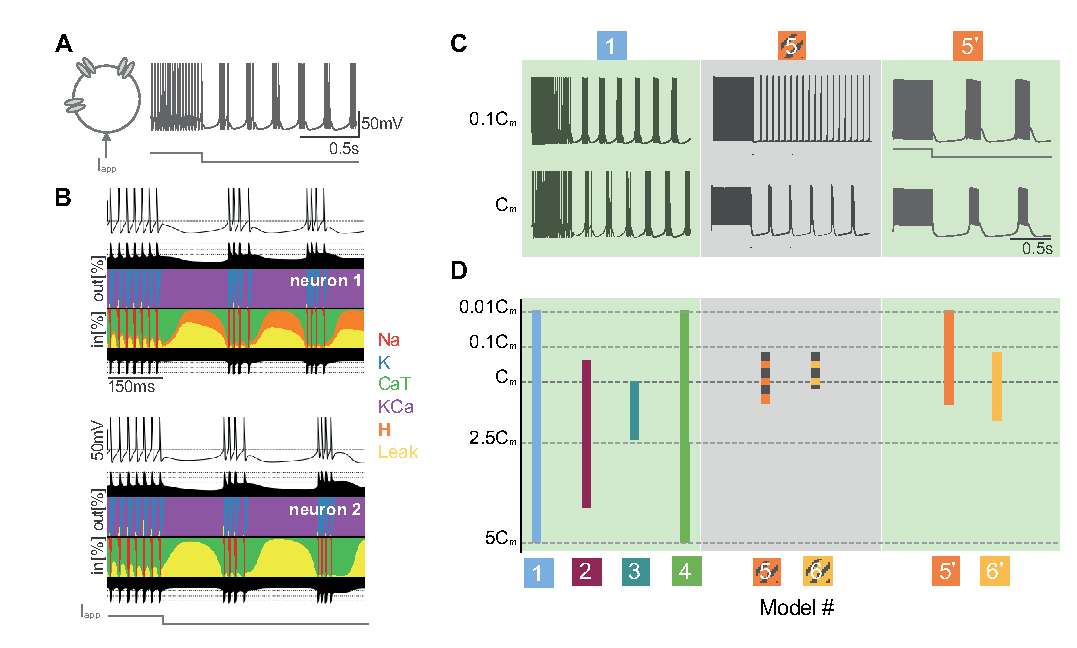
\includegraphics[scale=0.95]{fig/Plos/Fig1}
\caption{ {\bf Slow T-type calcium channel activation ensures model robustness against neuron variability at single-cell level. } \\
\textbf{A:} The cell switches from a regular tonic mode to a bursting mode when a hyperpolarizing current is applied, a typical response called hyperpolarized-induced bursting (HIB). \textbf{B:} Currentscape for a neuron model with two different sets of maximal intrinsic conductances. After 150ms, the two neurons are hyperpolarized, leading to a HIB. Under the membrane-time curve, the black surface shows respectively on the top and bottom total inward outward currents on a logarithmic scale (see \citep{alonso_visualization_2019}). Between the black surfaces, each color curve  reveals the contribution of one particular ionic current as the percentage of the total current during the simulation. Both neurons display the same firing pattern but this outcome is achieved by different combinations of ion channels densities. \textbf{C:} Models 1, 2, 3, 4, 5' and 6' are robust to a uniform scaling of all the maximal conductances, modeled by a change in membrane capacitance ($C_m$)(left panel). Models 5 and 6 are fragile to this parameter alteration. They lose the ability to switch (center panel). Restoring the slow CaT channel activation is enough to recover the robustness (right panel). \textbf{D:} Quantitative analysis of neuron model robustness to change in membrane capacitance. Each model is launched for a capacitance value varying from a hundredth to five times its nominal value. Models 1, 2, 3, 4, 5' and 6' cover larger parameter range. By contrast,  models lacking of slow CaT channel activation are fragile to membrane capacitance deviation. Replacing the instantaneous CaT channel activation by a slow activation turns these fragile models into more robust models. Hence, models 5' and 6' support larger variation of $C_m$. }
\label{fig:1}
%\end{adjustwidth}
\end{figure}


Experimental and computational studies have shown that a similar behavior or a similar firing pattern can emerge from neurons or circuits having very distinct intrinsic parameters 
\citep{alonso_visualization_2019, goldman_dependence_2000, marder_modeling_2002}. Fig~\ref{fig:1}B illustrates the membrane voltage time-course of a thalamic neuron model for two different sets of maximal intrinsic conductances under the control of an external hyperpolarizing current (see black curves). The firing pattern is similar in both parameter sets and shows the typical switch occurring in thalamic neurons. However, the corresponding currentscapes reveal a variability in the contributions of the different ionic currents \citep{alonso_visualization_2019}. A H-current (orange curve) is involved in the first neuron (top currentscape) while it is almost absent in the second neuron (bottom currentscape).  It shows that different combinations of ionic currents can lead to same firing pattern.  This simple experiment motivated the rest of this work; a computational model must be able to reproduce a desired outcome for a broad range of intrinsic parameters as it happens in biology.

Here, we studied the robustness of conductance-based models to parameter variations  with a special focus on the dynamics of the voltage-gated T-type calcium channel activation. The first four models (models 1 to 4) incorporate a \textit{slow} activation of the T-type calcium (CaT) channels while the last two models (models 5 and 6) fix the activation as an instantaneous event. This simplification is often encountered in neuronal modeling \citep{wang_multiple_1994, rush_analysis_1994, pospischil_minimal_2008, kubota_nmda-induced_2011, rubin_high_2004, smith_fourier_2000, amarillo_analysis_2015, golomb_synchronization_1994}. Indeed, it removes one differential equation, which decreases the simulation time - a computation intake that is non-negligible as soon as one moves toward network simulations. 



First, we investigated the impact of the CaT channel activation \textit{dynamics} in the model robustness at the single cell level. To do so, we simply tested the ability to reproduce the switch from tonic to burst by changing a single parameter in the model, namely, the capacitance membrane $C_m$. An alteration in this parameter substitutes a change in cell size or a uniform scaling of all maximal ionic conductances \citep{oleary_cell_2014, franci_robust_2018} . Fig~\ref{fig:1}C reveals the striking consequence for the model robustness when the capacitance is scaled by a factor 1/10. Models 1 to 4 (left panel) including the slow activation of T-type calcium channel are able to reproduce the hyperpolarized-induced bursting while models that assume this activation is instantaneous are fragile. Indeed, models 5 and 6 (center panel) loose the ability to switch from tonic to burst. To make the comparison as fair as possible, we have restored the slow dynamics of the CaT channel activation in models 5 and 6. We reconstructed a differential equation for the activation variable whose time constant is voltage-dependent. Models 5' and 6' are their respective modified versions.  The T-type calcium current previously described by $I_{CaT} = g_{CaT} \boldsymbol{m^a_{CaT, \infty}} h_{CaT} (V_m- V_{Ca})$ is replaced by $ I_{CaT} = g_{CaT} \boldsymbol{m^a_{CaT}(V_m)} h_{CaT} (V_m- V_{Ca})$ where $dm_{CaT}/dt = (m_{CaT,\infty}-m_{CaT})/\tau_{m_{CaT}}(V_m)$ (see \textcolor{red}{S1 Supplementary Material} Supplementary Material for details). This only modification  is sufficient to recover the desired firing activity, \textit{ie.} the switch from tonic to burst even for a division of the capacitance membrane by a factor of 10 (Fig~\ref{fig:1}C, right panel). 

This computational experiment has been reproduced for membrane capacitance values scaled from a hundredth to five times its nominal value (see \textcolor{red}{sec:methods} for details). Fig~\ref{fig:1}D reveals that models 1 to 4 are able to switch for a large range of capacitance values (see left panel). Models 5 and 6 are fragile and cover a tiny range around the nominal value ($C_m$) (center panel). Reinstating the slow dynamics of this channel bounces back the robustness as shown by the increase of the orange and yellow bars (right panel). Models 5' and 6' are able to generate the firing pattern switch typical in thalamic cells  given capacitance values for which models 5 and 6 are not able.

\subsection{Slow T-type calcium channel activation makes an isolated excitatory-inhibitory circuit  robust to neuromodulation and synaptic plasticity }
To extend our results obtained at the single-cell level, we moved to the circuit level. We built an isolated excitatory-inhibitory circuit of two neurons. These neurons are connected through AMPA, GABA\textsubscript{A} and GABA\textsubscript{B} connections to model the asymmetric coupling between a subpopulation of excitatory (E) cells and a subpopulation of inhibitory (I) cells 
\citep{guillery_thalamic_2002, mccormick_brain_2015}. This topology is a typical configuration in  the thalamus \citep{mccormick_sleep_1997, sherman_functional_1996}. The E-I circuit and its expected rhythmic network activity are  illustrated in Fig~\ref{fig:2}A (left and center panels). It is controlled by an external current injected on the inhibitory cell. Initially depolarized, the I-cell exhibits a tonic mode. The E-cell remains silent. As soon as the external current hyperpolarizes the I-cell; it deinactivates the T-type calcium channels, leading to a bursting mode. Then, thanks to the reciprocal connections, the circuit switches to a synchronous burst called the oscillatory mode. 

\begin{figure}[h!]
\centering
%\begin{adjustwidth}{-2in}{0.1in}
\includegraphics[scale=0.95]{fig/Plos/Fig2}
\caption{{ \bf Slow T-type calcium channel activation ensures model compatibility with neuromodulation and synaptic plasticity at the circuit level. } \\ \textbf{A:} (left) Two interconnected neurons (one excitatory neuron E and one inhibitory neuron I) under the control of an external current (I\textsubscript{app}), affected by neuromodulation (Nmod, pink spheres) and synaptic plasticity (Syn. Plast., in grayish blue).  (center) The external current initially depolarizes the inhibitory cell then hyperpolarizes it leading to a switch in the circuit rhythm into a synchronous bursting. (right) Voltage traces illustrating an asynchronous rhythm, undesired behavior in the circuit. 
\textbf{B:} Percentage of rhythmic networks observed in different neuron models as intrinsic variability increases. For each model, one thousand 2-cell circuits are generated with random ionic conductances varying from 10, 20 and 30$\%$ from their nominal values -mimicking the effect of neuromodulation, and synaptic conductances, randomly picked in a uniform distribution - mimicking the effect of synaptic plasticity.  Models 1 to 3 embedding a slow activation of T-type calcium channels are robust to parameter variability. Model 4 is robust at low variability than its performance is decreased due to its high number of ionic channels. Models 5 and 6 that assume an instantaneous T-type calcium channel activation are fragile: parameter variations disrupt the nominal rhythm.   Replacing the instantaneous activation into a slow activation restores the robustness as shown by models 5' and 6' (dashed orange and yellow bars).}
\label{fig:2}
%\end{adjustwidth}
\end{figure}

With a simple computational experiment, we studied the robustness of these network switches to changes in neuron intrinsic properties, mimicking the effect of neuromodulation (modeled by maximal conductances), and changes in synaptic weights, mimicking the effect of synaptic plasticity (modeled by the synaptic conductances). For each model, we started from an E-I circuit capable of generating a switch. Then, one thousand 2-cell circuits were simulated for different parameter sets of maximal intrinsic conductances and synaptic weights. The  maximal conductances varied within an interval of  10, 20 and 30$\%$ around their nominal values and the synaptic weights varied in a fixed range (see \textcolor{red}{sec:methods} for details). The percentage among the thousand 2-cell circuits  that have performed the rhythmic transition was evaluated for the three intervals of variability in each conductance-based model. A rhythmic network  is defined according to the firing pattern evolution shown in Fig~\ref{fig:2}A (center) representing a switch from silent-tonic to synchronous bursting while other activities are classified as an asynchronous rhythm, for example the pattern in  Fig~\ref{fig:2}A (right). Quantification of the firing pattern properties \textit{i.e.} frequencies in tonic and burst is available in \textcolor{red}{S1 Supplementary Material} Supplementary Material.

For a small intrinsic variability (10$\%$), Fig~\ref{fig:2}B shows that models 1 to 4 are robust to neuromodulation and synaptic plasticity. More than 800 sets of parameters allow the circuit to switch. The absence of slow positive feedback in models 5 and 6 has a dramatic consequence on the model robustness. One every two parameter sets in model 5 cannot reproduce the typical thalamic activity transition. Model 6 is even more fragile. However, restoring the dynamical cellular property significantly improves the robustness as shown in models 5' and 6'. 

For larger intrinsic variability (20$\%$ and 30$\%$), models 1 to 3 maintain their capabilities to switch for a broad range of intrinsic and synaptic parameter ranges. Model 4 can be considered apart. It is shrinking as the variability increases. This decrease in performance is likely related to its high number of conductances (about twice as much as the other models). Indeed, we are exploring a 14-dimension space since this model has 11 intrinsic conductances and 3 synaptic conductances. The parameter exploration for the other models occurs in a 7 to 9 dimension space reducing the model complexity. Models 5 and 6 have a similar number of intrinsic conductances as models 1 to 3 but they are extremely fragile to parameter changes. They are almost unable to perform rhythmic transition. The rhythm in an E-I circuit requires a precise tuning of intrinsic and synaptic parameters for models lacking of the slow kinetics of CaT channel activation. This computational choice makes the model incompatible with neuromodulation and synaptic plasticity.  Once again, their modified versions embedding the slow positive feedback (correlated to the slow activation of T-type calcium channels) have a better response to parameter perturbations. 


\subsection{A timescale separation between sodium and T-type calcium channel activations ensures compatibility between circuit switch, neuromodulation and synaptic plasticity}
So far, we have shown that modeling the T-type calcium channel activation with a slow kinetics drastically enhances the robustness of rhythmic switches at the cellular, and circuit levels. But one question remains: what does \textit{slow} mean, and how tuned does the activation kinetics need to be to achieve robustness? Indeed, there exists different subtypes of T-type calcium channels whose activation kinetics can greatly differ \citep{hille_ion_2001, perez-reyes_molecular_2003}.
To answer this question, we explored the  impact of incrementally varying T-type calcium channel activation kinetics in a similar computational experiment as done in Fig~\ref{fig:2}. We focused on models 1, 2, 3, 4, 5' and 6' that describe the opening of the T-type calcium channel with a first order differential equation $  dm_{CaT}(V_m) /  dt = ( m_{CaT, \infty} - m_{CaT})/ \tau_{m_{CaT}}(V_m) $. The variable $\tau_{m_{CaT}}$ is the voltage-dependent activation time constant and characterizes the dynamics of channel opening. We started from an isolated 2-cell E-I circuit connected via AMPA, GABA\textsubscript{A} and GABA\textsubscript{B} synapses.  The circuit is able to switch from tonic to burst at the nominal parameter values. Then, we added neuromodulatory effect - by varying intrinsic parameters, and synaptic plasticity - by changing extrinsic parameters. We built four hundred 2-cell circuits whose maximal ionic conductances and synaptic conductances were randomly picked in an interval of 20$\%$ around their basal values. Here, the novelty was to play with the time constant of CaT channel activation $\tau_{m_{CaT}}$  of the two neurons (see Fig~\ref{fig:3}A). 

Fig~\ref{fig:3}B is a comparative table between time constants associated to sodium channel activation $\tau_{m_{Na}}$, T-type calcium channel activation $\tau_{m_{CaT}}$ and inactivation $\tau_{h_{CaT}}$ evaluated at their threshold voltage (see \textcolor{red}{sec:methods} for details). It points out the quantitative differences between models. Here, we were investigating the choice made for $\tau_{m_{CaT}}$ with respect to $\tau_{m_{Na}}$ and $\tau_{h_{CaT}}$. To do so, the time constant $\tau_{m_{CaT}}$ was scaled by several multiplicative factors from  0.01  to 100 times its nominal value. The smallest the coefficient, the fastest the CaT channel activation. For each scaled CaT time constant, we tested the model capability to switch from tonic to burst when the I-cell is hyperpolarized. Among the 400 tested circuits, the percentage of rhythmic circuits is placed on the y-axis (see Fig~\ref{fig:3}C). The x-axis is on a logarithmic graduation. 

\begin{figure}[!h]
%\begin{adjustwidth}{-2.45in}{-0.25in}
%\centering
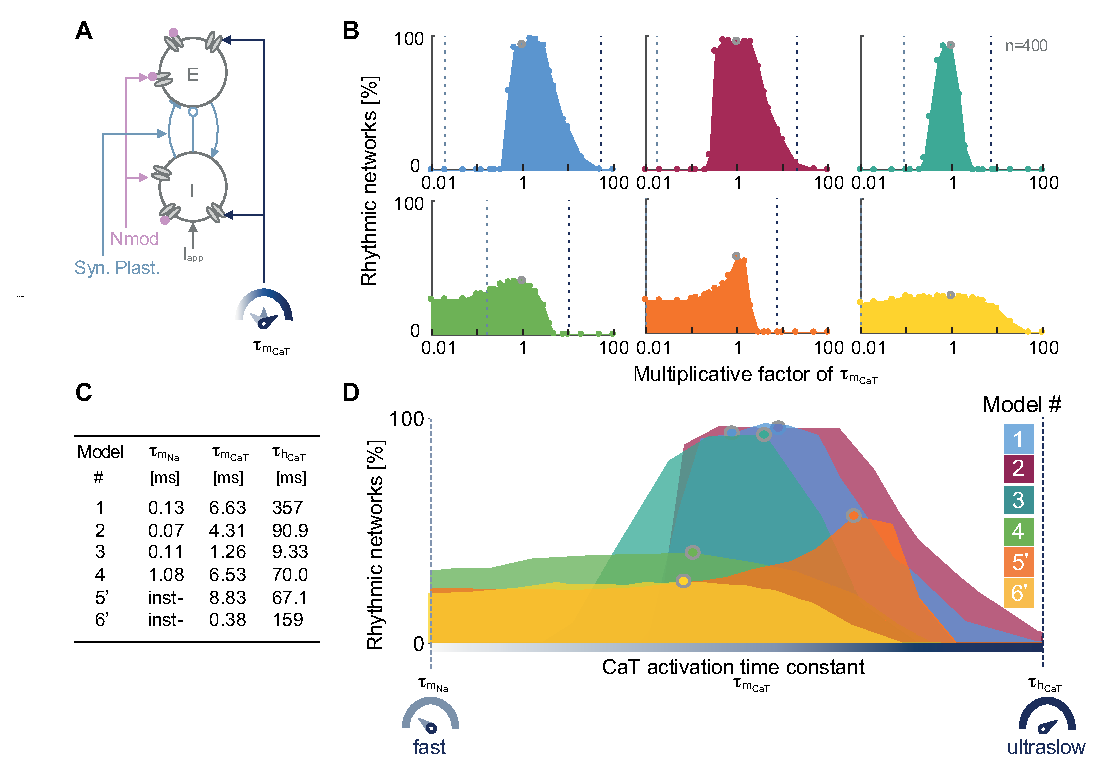
\includegraphics[scale=0.95]{fig/Plos/Fig3}
\caption{{\bf The physiological \textit{slow} timescale of T-type calcium channel activation guarantees compatibility between circuit switch, neuromodulation and synaptic plasticity.}\\ \textbf{A:} For each model, 400 E-I 2-cell circuits are built from scaled intrinsic and synaptic conductances picked in a uniform range of $\pm$ 20 $\%$ around their nominal values to mimic neuromodulation and synaptic plasticity.  These same 400 circuits are then simulated for a varying  CaT channel activation time constant ($\tau_{m_{CaT}}$). \textbf{B:} Comparison table between the time constants associated with sodium channel activation ($\tau_{m_{Na}}$), CaT channel activation and CaT channel inactivation ($\tau_{h_{CaT}}$). 
\textbf{C:} Effect of a varying CaT channel activation time constant on the switching capability in a 2-cell circuit for models 1, 2, 3, 4, 5' and 6'. The y-axis quantifies the percent of rhythmic networks among the 400 simulated random circuits under different values of $\tau_{m_{CaT}}$, scaled by a multiplicative factor varying from 0.01 to 100. The performance associated with the nominal (resp. scaled) CaT channel activation is depicted with a gray circle (resp full circle). The sodium channel activation (resp. CaT channel inactivation) time constant is marked with the left (resp. right) dashed vertical line.   
\textbf{D:} Each model is superposed between a window bounded on the left (resp. right) by the sodium channel activation (resp. CaT channel inactivation) time constant.  The CaT activation time constant must remain confined in the \textit{slow} timescale in order to guarantee model robustness to neuromodulation and synaptic plasticity. }
\label{fig:3}
%\end{adjustwidth}
\end{figure}

When the multiplicative factor is equal to one (marked by the gray circle), it indicates the CaT channel activation time constant initially designed for each model. The sodium channel activation time constant $\tau_{m_{Na}}$ and the CaT channel inactivation time constant $\tau_{h_{CaT}}$ are also drawn for each model in dashed lines (respectively $\tau_{m_{Na}}$ on the left and $\tau_{h_{CaT}}$ on the right). They are evaluated at their threshold voltage (see \textcolor{red}{sec:methods} for details). They respectively indicate the \textit{fast} and the \textit{ultraslow} timescale. For models 5' and 6', the sodium current activation is instantaneous.  For model 6',  the CaT channel inactivation does not appear on the graph since it is greater than 100 times its activation (see Table in Fig~\ref{fig:3}B).

The outcome of this computational experiment is compelling. Fig~\ref{fig:3}C reveals that models are robust to neuromodulation and synaptic plasticity when the timescale of the CaT channel is situated in a slow range. The meaning of slow stands by itself; it is bounded  between the fast kinetics of the sodium channel activation and the ultraslow kinetics of CaT channel inactivation. For each model, the peak of robustness lies between these two timescales. The bump-shaped surface shows a relatively large width. It points out that the activation kinetics do not need to be perfectly equal to one specific value between the fast and ultraslow regions. But these kinetics just need to be included within the slow timescale range. However, as soon as the kinetics moves too far from this interval, the robustness loss is abrupt.

To go further in the analysis, the six models were superposed on each other by normalizing the logarithmic x-axis on Fig~\ref{fig:3}D. The left (resp. right) boundary is the time constant of the sodium channel activation (resp. CaT channel inactivation); namely, the fast and the ultraslow timescales.  The number of rhythmic circuits is enhanced when the CaT activation occurs at a timescale slower than the sodium activation and faster than the CaT inactivation as highlighted by the bump-shaped surface. Modeling the CaT channel opening at a slow timescale guarantees the compatibility between neuromodulation, synaptic plasticity and switches in brain states. Indeed, the compatibility relies on the presence of a \textit{slow positive feedback} at the cellular level, as mentioned above. 


Model 4 maintains a steady robustness even if the CaT channel activation is accelerated. This can be explained by the presence of another source of slow positive feedback such as a slowly activating L-type calcium channels (see \textcolor{red}{S1 Supplementary Material} Supplementary Material for more details about model 4). Models 5' and 6' display a modest robustness for a fast opening of the CaT channel. These models were initially designed to operate for an instantaneous activation. However, the favorable operating point is preferably at a slow timescale. 

If the kinetics of the CaT channel opening slows down too much (meaning we are moving to the right on the x-axis), it reaches the same timescale as its inactivation. In other words, the activation gate opens while the inactivation gate closes leading to a zero flux of calcium ions. The kinetics of CaT channel activation must be slow but not too slow.

\subsection{A timescale separation between sodium and T-type calcium channel activations promotes robustness of network states in large heterogeneous populations}
From an isolated E-I circuit of two neurons, we built a larger network whose topology is emblematic of the thalamus, illustrating the interaction between relay neurons and the reticular nucleus. This population interaction is involved in state regulation such as the transition from wakefulness to sleep \citep{mccormick_sleep_1997, murray_sherman_tonic_2001}. We replicated the two previous computational experiments performed at the circuit level, now on a neuronal population. To do so, we started with a 200-cell network where the population of 100 excitatory neurons  is identical to the population of 100 inhibitory neurons. We neglected intra-population interaction, and we assumed all-to-all connectivity between the two populations. The E-cells projected AMPA synapses to all the I-cells and conversely, the I-cells were connected to the E-cells via GABA\textsubscript{A} and GABA\textsubscript{B} synapses. All the synaptic weights linking the neurons together were identical. An external current was exerted on the inhibitory cells (see Fig~\ref{fig:4}A). Hyperpolarizing this current caused a cellular switch and drives the neurons in a synchronous bursting mode as previously shown with the isolated E-I circuit in Figs~\ref{fig:2}A and \ref{fig:4}B (voltage traces,  two top curves) \citep{drion_switchable_2018}. This change in cellular firing pattern is translated by an oscillatory behavior at the network level. This oscillatory state can be visualized by computing the local field potential (LFP) of the neuron population.  LFP is measured as the sum of synaptic activity in a neuronal population (see Fig~\ref{fig:4}B,  third curve). When the current hyperpolarizes the I-cells, the synaptic current is remarkably modified and reveals a stronger activity. The spectrogram of the LFP shows that the hyperpolarizing current turns on the mean-field rhythmic activity marked by a strong power LFP frequency band (see Fig~\ref{fig:4}B, frequency-time image at the bottom). For each model, the homogeneous network is able to switch from an active state to an oscillatory state. 

\begin{figure}[h!]
%\begin{adjustwidth}{-2in}{0.1in}
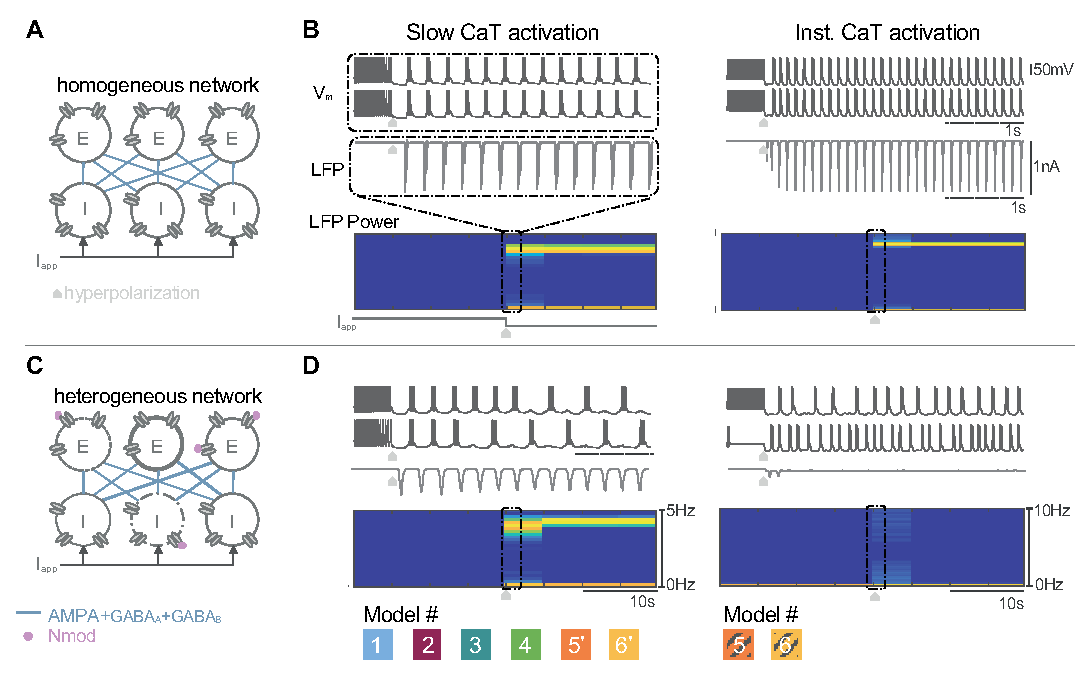
\includegraphics[scale=0.95]{fig/Plos/Fig4}
\caption{ {\bf Slow T-type calcium channel activation guarantees robust network switch independent on the population heterogeneity.}\\ \textbf{A:} A 200-cell network is built with the same neuron model; 100 excitatory cells connected via the AMPA synapses to 100 inhibitory cells projecting back GABA\textsubscript{A} and GABA\textsubscript{B} synapses. The network is homogeneous. All neurons have the same channel densities and the same synaptic weights. \textbf{B:} Voltage traces of two inhibitory cells (two top curves), time-course (third curve) and frequency-time graph (bottom spectrogram) of the local field potentials (LFPs) of the inhibitory neuron population for the homogeneous network. Hyperpolarization of the inhibitory neurons turns on the mean-field rhythm activity of the population depicted by a synchronous bursting at the cellular level, a oscillating synaptic activity shown on the LFP time course whose frequency is shown by the high power LFP frequency band on the spectrogram. \textbf{C:}  A heterogeneous 200-cell network is built to take into account neuromodulation, cell variability, more representative topology and synaptic plasticity. Each ionic and synaptic conductance is randomly picked in a given range around its nominal value (see \textcolor{red}{sec:methods} for details).   \textbf{D:} (left panel) Only models 1,2,3,4 5' and 6' display the switch in the mean field rhythm of the population marked with an oscillatory LFP time-course (third curve) and a significant power band in the spectrogram (bottom). (right panel) Models 5 and 6 that lack slow CaT channel activation are fragile to the network topology and the heterogeneity. Switch in population rhythm is recovered when the slow regenerativity is restored (models 5' and 6').} 
\label{fig:4}
%\end{adjustwidth}
\end{figure}

However, a perfect network with identical neurons and identical synaptic weights is not consistent with reality. Each neuron differs from its neighbor with different intrinsic parameters such as the cell size or the densities of ionic channels. In addition, connections between neurons are neither identical nor static. Therefore, we explored the model ability to maintain switch in brain states in presence of cellular heterogeneity and its independence on network topology \citep{drion_switchable_2018, drion_cellular_2019}. To do so, we built a 200-cell network where each neuron is different and the connectivity is uneven (see Fig~\ref{fig:4}C). The intrinsic and synaptic parameters were randomly picked in a given interval (see \textcolor{red}{sec:methods} for details). Fig~\ref{fig:4}D shows the astonishing contrast between the stability of models including the slow CaT channel activation (see left panel) and the fragility of  models lacking of this property (see right panel). Models 1 to 4, 5' and 6' are still able to generate a switch into a synchronous burst as shown in Fig~\ref{fig:4}D (left). Due to intrinsic and synaptic variabilities, the voltage recordings from two I-cells are more realistic (two top traces). Even if each cell is not perfectly bursting at each cycle, the summation of the synaptic activity shown by the LFP curve is oscillating(third curve). The frequency of this oscillation is quantified in the spectrogram (bottom frequency-time graph).  
Models 5 and 6 are able to switch from an active state to an oscillatory when the network is homogeneous and the connectivity is perfectly balanced. However, as soon as the network is changed into a more realistic configuration, these models cannot preserve switches in brain states as shown by the asynchronous voltage-traces and the flat LFP curve translated by the absence of a marked power band in the spectrogram (see Fig~\ref{fig:4}D right panels). 

Models 1 to 3 show a marked power band in their spectrogram when intrinsic parameters vary in an interval  of 20$\%$ around their nominal values. Once again, model 4 is  less robust, certainly due to its high number of conductances. It continues to switch for an intrinsic variability of 10$\%$. Model 5 (resp. model 6)  does not tolerate a variability of 20$\%$ (resp. 5$\%$).  When the slow activation of T-type calcium channels is reestablished, models 5' and 6' switch from an active state to an oscillatory state at the same level of variability that the initial model was fragile. This modeling modification leads to a neuron model robust to cell variability and that does not rely on the network topology. \\

To go further, we explored once again  the relevance of respecting physiological timescale separation in ionic current modeling but this time at the population level. To do so, we built a 200-cell network with 100 excitatory cells connected to 100 inhibitory cells via AMPA, GABA\textsubscript{A} and GABA\textsubscript{B} synapses.  Models 1,2, 3, 4, 5' and 6' were switching their network state under a hyperpolarizing current for a homogeneous and a heterogeneous configuration, as shown in Fig~\ref{fig:4}B and \ref{fig:4}D (left panels).  Here, we tested which kinetics provides robustness to network heterogeneity. The CaT activation time constant $\tau_{m_{CaT}}$ of the 200 neurons was scaled by several multiplicative factors ranging from an eighth to eight times its nominal value. In addition, cellular and synaptic variabilities were introduced by randomly picking the maximal intrinsic and extrinsic conductances of each neuron in a given interval around their nominal values following a uniform distribution (see Fig~\ref{fig:5}A).  These heterogeneous networks were constructed with parameters varying in an interval whose width was ranging from 0 to 50$\%$ with a step of 5$\%$. At each scaled $\tau_{m_{CaT}}$, we tested the maximal possible variability width at which the heterogeneous network is able to switch.  For example, we built the 200-cell network whose maximal ionic and synaptic conductances were picked in a range of 20$\%$ around their initial values. Then, we simulated the network under the control of an hyperpolarizing current at different scaled $\tau_{m_{CaT}}$. We finally checked for each timescale if the given heterogeneous network was switching or not, by analyzing its LFP activity. The network was switching if the time course of neuron population LFP displayed an oscillatory behavior in the hyperpolarized state and if its spectrogram was marked by a strong power band (see Fig 5B). We continued to increase the variability interval to quantify the correlation between the timescale and its robustness to cellular heterogeneity and uneven topology.

\begin{figure}[h!]
\centering
%\begin{adjustwidth}{-2in}{0.1in}
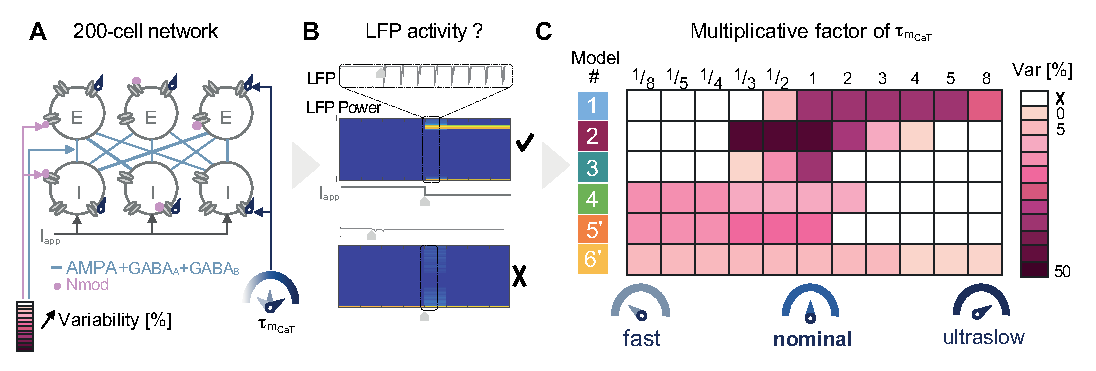
\includegraphics[scale=0.95]{fig/Plos/Fig5}
\caption{ {\bf Comparison between fast, slow or ultraslow T-type calcium channel activation in generating robust mean-field activity transition. } \\
\textbf{A:} A 200-cell network with 100 excitatory neurons and 100 inhibitory neurons connected via AMPA,  GABA\textsubscript{A} and GABA\textsubscript{B} synapses under the control of an hyperpolarizing current.  The intrinsic and extrinsic parameters are respectively affected by neuromodulation and synaptic plasticity; their values are randomly picked in a given interval (namely variability). The CaT channel activation time constant $\tau_{m_{CaT}}$ of each neuron is scaled by a multiplicative factor. \textbf{B:} At each scaled time constant, we check if the heterogeneous network is switching by analyzing the LFP activity. If the LFP timecourse presents a strong activity and its spectrogram shows a marked power band, the network displays an oscillatory state during the hyperpolarization state.  \textbf{C:} The table summarizes the largest variability width at which the network presents a switch in its mean-field activity for several scaled time constants. Respecting the slow timescale of the CaT channel activation guarantees the switch in network rhythm compatible with variability in channel densities and synaptic weights. Driving the CaT channel activation to a fast or ultraslow timescale makes models more fragile to network topology and heterogeneity. }
\label{fig:5}
%\end{adjustwidth}
\end{figure}

Fig~\ref{fig:5}C summarizes the model robustness at each scaled CaT time constant. It confirms our previous result; accelerating or decelerating the CaT channel opening makes the six models fragile to heterogeneity. In models 1 to 3, the best operating point to set the CaT time constant is confined between the fast timescale and the ultraslow timescale as shown by the darker zone. It enhances the model capability to switch in presence of cellular heterogeneity and synaptic plasticity. Model 4 is not really robust due to its high number of ionic currents. It is also assumed to embed another source of slow regenerativity helping it to operate at a faster timescale.  As exhibited in Fig~\ref{fig:3}C for an isolated 2-cell circuit, models 5' and 6' also maintain a certain ability to switch even at a faster timescale because they were initially designed to operate at an instantaneous opening of CaT channels. As adapted versions of models designed to switch with an instantaneous T-type calcium activation, their robustness is lower than models 1 to 3 in all parameter ranges. 

Overall, Figs~\ref{fig:3} and \ref{fig:5} reveal the importance of considering the physiological kinetics range of ion channel gating in computational models and especially the timescale separation between the different ionic currents. Getting rid of the slow dynamics of the T-type calcium channel activation disrupts the timescale separation with sodium channel activation. It removes an important biological property of this neuron type and thus, disturb its ability to change its firing pattern under a hyperpolarization in presence of neuromodulation and synaptic plasticity. This deficiency is transposed at the population level as shown by the inability to turn on the mean-field activity as soon as the cellular heterogeneity and unbalanced connectivity are increased.

\subsection{Slow T-type calcium channel shapes a robust phase portrait}
How does the kinetics of T-type calcium channel shapes the phase portrait? To answer this question, we reduced the different high-dimensional models following the protocol presented in \citep{drion_dynamic_2015}. The protocol is based on the decomposition of each variable into their role in a fast, slow and ultraslow timescale using a logarithmic distance \citep{drion_dynamic_2015}.  It allows us to reduce the different conductance-based models in a systematic and rigorous manner in order to obtain three dimensional models with three variables: the membrane voltage of the reduced model $V$,  the slow variable $V_s$ and the ultraslow variable $V_u$.  The contribution of the activation or inactivation channel variables ($m_i(V)$ or $h_i(V)$ contracted as $X(V)$ to ease the reading) is projected on these three variables. The voltage-dependent gating variable is transformed into a weighted sum of three terms associated with the three timescales where the weights are voltage-dependent.  The weighted sum is written as: $X(V) = w_{fs}^{X}(V) X_{\infty}(V) + (w_{su}^{X}(V) - w_{fs}^{X}(V))X_{\infty}(V_s) + (1-w_{su}^{X}(V)) X_{\infty}(V_{u}) $ where $w_{fs}^{X}(V)$ is the contribution of the gating variable on the fast time-scale,  $(w_{su}^{X}(V)- w_{fs}^{X}(V))$ is the contribution on the slow time-scale and $(1-w_{su}^{X}(V))$ is the contribution on the ultraslow time-scale.  Therefore, the 3D reduced model is described by the following differential equations: $ C_m dV/dt = - \sum I_{ion} + \text{I}_\text{{app}}$, $dV_s/dt = (V - V_s)/ \tau_{m_K}(V)$ and $dV_{u}/dt = (V - V_{u})/\tau_{h_{CaT}}(V)$. The time-constant of the sodium activation $\tau_{m_{Na}}(V)$ paces the fast time-scale,  the time-constant of the potassium activation $\tau_{m_K}(V)$  paces the slow time-scale and the inactivation of the T-type calcium channel $\tau_{h_{CaT}}(V)$ paces the ultraslow time-scale.


In this work, we focus on the timescale attributed to the activation to the T-type calcium channel.  We investigated the distortion of the phase portrait geometry when this time constant is increased or decreased.  Fig~\ref{fig:6} shows the analysis of a conductance-based model reduced under three different conditions applied on T-type calcium channel activation, when it is considered as fast,( $\tau_{m_{CaT}}(V)/50$ - left column), slow (nominal $\tau_{m_{CaT}}(V)$ - center column) and ultraslow ($50 \tau_{m_{CaT}}(V)$ - right column).  Fig~\ref{fig:6}A shows the voltage time-courses when a hyperpolarizing current is applied to reproduce a hyperpolarized-induced bursting. Fig~\ref{fig:6}B exhibits the fast-slow phase portrait drawn at a given time (indicated by (1) in the voltage trace) in order to compare the tonic mode under the three conditions.  Fig~\ref{fig:6}C is also the fast-slow phase portrait drawn this time at the saddle node bifurcation (indicated by 2 in the voltage trace, see \textcolor{red}{sec:methods} for details). Videos of the membrane voltage time course, the associated phase portrait including the evolution of the nullclines and the trajectory for the different kinetics are available in \textcolor{red}{S1 Video} Video (fast),  \textcolor{red}{S2 Video} Video (slow) and \textcolor{red}{S3 Video} Video (ultraslow).  In \textcolor{red}{S1 Supplementary Material} Supplementary Material, simulations of the reduced models 2, 5', 6 and 6' are available.

\begin{figure}[h!]
\centering
%\begin{adjustwidth}{-0.3in}{0 in}
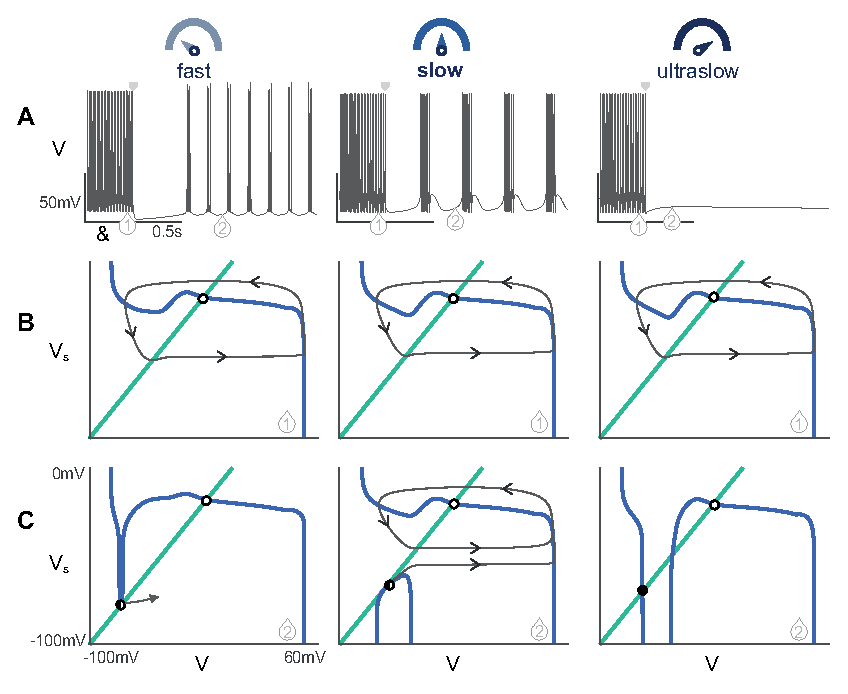
\includegraphics[scale=1]{fig/Plos/Fig6}
\caption{ {\bf Distortion of the phase portrait when the T-type calcium channel activation is considered as fast, slow or ultraslow.  } \\
\textbf{A:} Voltage traces of a reduced model under the three conditions during a hyperpolarized-induced bursting. The square arrow indicates the hyperpolarizing current step. When the CaT activation is ultraslow, the model is not able to switch from tonic to burst.
\textbf{B:} Comparison of the portrait geometry during tonic mode (arrow 1) under the three timescales.  V-(resp. Vs-) nullcline is sketched in blue (resp. green).  The unstable fixed point is marked in open circle. The limit cycle followed by the trajectory is sketched in gray. The timescale chosen for the CaT channel activation is not affecting the tonic mode.
\textbf{C:} Comparison of the portrait geometry during burst mode (at the saddle node bifurcation, arrow 2) under the three timescales. The stable fixed point is marked as a filled black circle and the saddle point meeting the stable fixed point is indicated by the black half-circle.  At the ultraslow timescale (right), there is no saddle-node bifurcation,the V-nullcline is distorted into its hourglass shape trapping the trajectory into its stable fixed point.  (left) For the \textit{fast} CaT activation channel, the V-nullcline presents only the upper branch where the saddle node bifurcation occurs (center) For the \textit{slow} activation, the V-nullcline exhibits a lower branch. This branch robustly separates the silent region and the spiking region of bursting. Videos of the simulations under the three conditions are available in \textcolor{red}{S1 Video} Video (fast), \textcolor{red}{S2 Video} Video (slow) and \textcolor{red}{S3 Video} Video (ultraslow).}
\label{fig:6}
%\end{adjustwidth}
\end{figure}


First,  the timescale chosen for CaT channel activation has no influence on the tonic mode.  The reduced model is similarly spiking under the three conditions.  The phase plane associated to the discharge mode is not affected.  It shows the classical limit cycle extensively studied in spiking models.  The trajectory is trapped in the limit cycle around the unstable fixed point present on the expected N-shaped V-nullcline.  Second, considering the T-type calcium channel activation as slow as its inactivation removes the ability of the model to switch from tonic to burst (third column).  The V-nullcline has a hourglass shape showing the influence of the inactivation of the T-type calcium channel (as shown in \citep{drion_novel_2012}). The trajectory is attracted by the stable fixed point at the hyperpolarized state. This highlights a lack of depolarizing current, which is due to the simultaneous activation and inactivation of T-type calcium channels. 

Finally,  the most interesting result is the comparison of the phase portraits during burst mode in the case of the fast activation (Fig~\ref{fig:6}C-left) versus the slow activation of T-type calcium channel (Fig~\ref{fig:6}C-center).  We drawn both reduced models at the saddle node (SN) bifurcation (see \textcolor{red}{sec:methods} for details).  The main difference comes from the V-nullcline: for the fast activation of CaT channel, the phase portrait is qualitatively similar to the one in spiking mode. For the nominal activation timescale, the phase portrait qualitatively changes by the appearance of a lower branch in the V-nullcline, which permits to robustly separate the silent region (which sits on the lower branch) and the spiking region of bursting (which sits on the upper branch). 

Therefore, speeding up the activation of the T-type calcium activation disrupts the ability of T-type calcium channel deinactivation to qualitatively change the phase portrait structure from robust spiking to robust bursting in response to hyperpolarization \citep{drion_novel_2012,franci_balance_2013, franci_modeling_2014}. The same behavior is observed in all models regardless of their quantitative differences. This remarkable distortion of the phase portrait when $\tau_{m_{CaT}}$ is scaled from the fast timescale to the ultraslow is shown in \textcolor{red}{S4 Video} Video.

The consequence on robustness and tunability of this qualitative change is illustrated in Fig~\ref{fig:7}. This figure compares the phase portrait of the reduced version of model 1(embedding a slow T-type calcium channel activation) and the reduced version of model 5 (embedding an instantaneous T-type calcium channel activation) when the capacitance membrane is divided by three.  We have chosen the membrane capacitance for two reasons. First, as done in Fig~\ref{fig:1} it is a suitable parameter to test the model robustness to a uniform scaling of maximal conductances or mimicking a change in cell size. Then, from a dynamical viewpoint,  the membrane capacitance sets the timescale of the voltage equation. Reducing its value does not affect the nullcline shape nor the fixed point locations but solely affects the vector field.

\begin{figure}[h!]
\centering
%\begin{adjustwidth}{-2in}{0.1in}
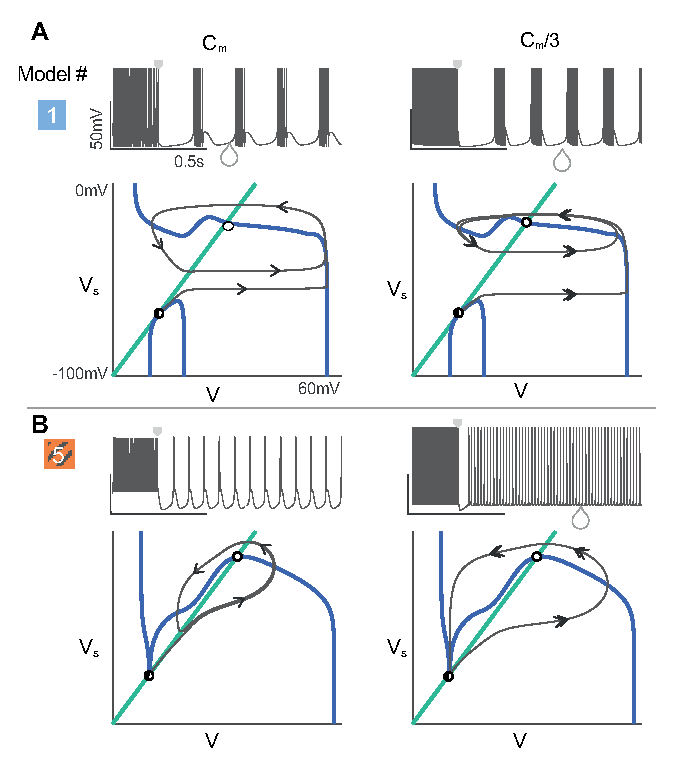
\includegraphics[scale=1]{fig/Plos/Fig7}
\caption{ {\bf The slow activation of T-type calcium channel reveals the appearance of a lower branch in the V-nullcline providing robustness to parameter variation. }\\
\textbf{A-B:} (top) Recording of the membrane voltage during a hyperpolarized-induced bursting (bottom). Phase portrait at the saddle node bifurcation. V-(resp. Vs-) nullcline is sketched in blue (resp. green).  The square arrow indicates the hyperpolarizing current step. The unstable fixed point is marked by an open circle and the saddle point meeting the stable fixed point is indicated by the black half-circle. The trajectory is sketched in gray and the arrow indicates the speed along the x-axis. (left to right) the membrane capacitance is divided by 3.  The velocity along the x-axis is increased. 
\textbf{A:} The V-nullcline exhibits a lower branch making the phase portrait robust to membrane capacitance variation due to the sharp separation between the limit cycle and the hyperpolarized state.
\textbf{B:} When the membrane capacitance is divided by three, the reduced model 5 is no more able to switch from tonic to burst. Small deviations destroy the rest-spike bistability. Videos of the different simulations are available in \textcolor{red}{S5 Video} to \textcolor{red}{S8 Video} Videos}
\label{fig:7}
%\end{adjustwidth}
\end{figure}

Both models are able to switch from tonic to burst at the nominal value $C_m$, but they do so through two different mechanisms. Model 1 uses the appearance of a lower branch in the V-nullcline (see Fig~\ref{fig:7}A,left), whereas model 5 relies on the presence of a region where the timescale separation between the fast and slow timescales is inverted, \textit{i.e. } the slow timescale becomes faster, which is illustrated by vertical trajectories and vector field away from the nullclines (see Fig~\ref{fig:7}B,left). Both mechanisms permit to generate bursting. However, the second mechanism relying on such a dynamical property, it is very fragile to changes in membrane parameters: a reduction of the membrane capacitance removes this region of inverted time-scale separation, hence disrupts the ability to burst (Fig~\ref{fig:7}B,right). The mechanism based on the lower branch of the V-nullcline is structural, hence robust to changes in dynamics created by changes in membrane properties (Fig~\ref{fig:7}A,right).  Videos of the simulations are available in \textcolor{red}{S5 Video} Video (model 1, $C_m$), \textcolor{red}{S6 Video} Video (model 1, $C_m/3$), \textcolor{red}{S7 Video} Video (model 5, $C_m$) and \textcolor{red}{S8 Video} Video (model 5, $C_m/3$).

The reader is referred to \citep{drion_novel_2012, franci_organizing_2012,franci_balance_2013}  for a detailed explanation of the origin and the effect of the lower branch present in the V-nullcline in model with the slow CaT calcium channel activation.  More explanations about the robustness and tunability provided by the presence of the lower branch in the V-nullcline versus the classical N-shape are presented in \citep{franci_robust_2018}.



\section{Discussion}
\subsection{The physiological timescale separation between sodium and T-type calcium channel activations.}
A quotation from Bertil Hille’s book \citep{hille_ion_2001}, " The time course of rapid activation and inactivation of T-type $I_{Ca}$ has been described by an $m^3h$ model like that for $I_{Na}$ (Coulter et al.1989) \citep{coulter_calcium_1989} ; (Herrington and Lingle 1992) \citep{herrington_kinetic_1992}, but the derived time constants $\tau_m$ and $\tau_h$ are 20 to 50 times longer than those for $I_{Na}$ of an axon at the same temperature.", highlights a physiological timescale separation between sodium and T-type calcium channel gating kinetics. T-type calcium channel presents of portfolio of activation kinetics depending on their isotype (i.e. Ca\textsubscript{V}3.1, Ca\textsubscript{V}3.2 or Ca\textsubscript{V}3.3), but all isotypes share the property of activating a timescale slower than sodium channels: the activation time constant ranges between 1ms and 50ms  
\citep{klockner_comparison_1999,  cain_contributions_2010,  chemin_specific_2002,  clapham_international_2005,  perez-reyes_molecular_2003,  frazier_gating_2001, choi_altered_2015}. By contrast, the activation time constant of sodium channel is lower than 1ms  \citep{hodgkin_quantitative_1952,  gilly_fast_1997, reckziegel_electrophysiological_1998,  hille_ion_2001}. As explicitly shown with these numbers, there is one order of magnitude between these two gating time constants.

T-type calcium channels play a major role in oscillations generated, sustained or propagated by the thalamic circuit such as in sleep or in epilepsy. They are known to be modulated by several signaling cascades or also targets of several experimental and clinical drugs 
\citep{perez-reyes_molecular_2003,zamponi_physiology_2015, chen_role_2014,blesneac_phosphorylation_2015,lambert_modulation_2008,huc_regulation_2009, traboulsie_subunit-specific_2007}. These modulations can change the kinetics of this channel activation.  Our computational experiments are physiologically relevant since modifying the activation kinetics can lead to undesired behavior. 


\subsection{Modeling T-type calcium channel activation in conductance-based models}
In a conductance-based model, the opening of an ion channel is represented by a voltage-dependent gating variable. This variable is described with a first order differential equation whose time constant is also voltage-dependent. In this paper, we investigated the kinetics chosen for the T-type calcium channel activation with respect to sodium channel activation. In other words, we compared these time constants with respect to each other. 

There is a growing trend to design T-type calcium channel activation as the equivalent of a sodium channel activation. It often based on the fact that these two channels activate on a faster timescale than their own inactivation. For example in the published paper associated to model 5, it is said that "the activation variable [of T-type calcium channel] $s$ is relatively fast and is replaced by its equilibrium function. (...) The activation kinetics [of the sodium current] being fast, the variable $m$ is replaced by its equilibrium function (...) " \citep{wang_multiple_1994}. However, in the original version published three years before, the activation of T-type calcium channel was not at the same timescale as the sodium channel activation \citep{wang_model_1991}. In the same way for model 6, it is written "We employ a simplified version of the quantitative model originally formulated by Wang et al. (1991). Activation $s$ is rapid, and inactivation $h$ is relatively slow, (...) activation is assumed to be instantaneous. " \citep{rush_analysis_1994}. The similar simplification occurs for model 3 published in 1998: ten years later, the author mentioned "Note that the activation variable $s$ is considered here at steady-state, because the activation in fast compared to inactivation. This T-current model was also used with an independent activation variable (\citep{destexhe_dendritic_1998}), but produced very similar results as the model with activation at steady-state" \citep{pospischil_minimal_2008}. 

Modeling the T-type calcium channel activation on the same timescale as the sodium channel activiation is a modeling simplification that does not only appears in models of thalamic neurons. For example in basal ganglia, subthalamic neurons are excitatory neurons projecting to inhibitory globus pallidus neurons. These neurons present a switch in firing activity that leads to different brain states, particularly relevant in movement generation and in Parkinson's disease \citep{uhlhaas_neural_2006, bevan_move_2002, gatev_oscillations_2006, kuhn_event-related_2004, brown_basal_2005, swann_deep_2011}. Subthalamic neurons also embed T-type calcium channels. Once again, it is common to see that the activation of sodium and T-type calcium channels are modeled on the same timescale  or even considered as instantaneous \citep{kubota_nmda-induced_2011, terman_activity_2002, rubin_high_2004}. 
In both situations, these models are operational. It means that differentiating the sodium and T-type calcium channel activations is \textit{not indispensable to reproduce} discharge modes. Those models are able to fire in tonic and burst. This timescale separation between the activation of these two different channels is neglected because it seems to be a computational detail.  Figs~\ref{fig:3},  \ref{fig:5} and \ref{fig:7} confirm that models initially considering a fast activation of T-type calcium channel can perform the desired activity.  However, our results stress the crucial importance of this timescale separation for the \textit{robustness} in network switches.  The optimum operating timescale for T-type calcium channel activation is located between the fast activation of sodium channels and the ultraslow inactivation of T-type calcium channels. 

As mentioned earlier, both channels have different electrophysiological properties. Assuming the T-type calcium channel activation as fast as sodium channel activation means that it is just a current summation. This has for consequence to drastically reduce the ability of generating a robust network activity as shown in our computational experiments. \\

\subsection{Compatibility between switches in brain states, synaptic plasticity and neuromodulation}
Neuronal oscillations, synaptic plasticity and neuromodulation are hot topics in neuroscience since they are building blocks for information processing, learning, memory or adaptability. Studying the interaction between them requires computational models that generate \textit{robust} activity even if the synaptic connectivity and the endogenous parameters are altered. 


Altogether, this paper reveals that the \textit{robustness} in the brain state switches in presence of cellular variability, heterogeneity at the network level is \textit{correlated with the timescale separation} between sodium and T-type calcium channel activations. Despite the quantitative differences between the models, this timescale separation makes the rhythmic transition compatible with temporal variability and spatial heterogeneity induced by regulatory functions like neuromodulation, synaptic plasticity and homeostasis. In particular, triggering oscillations without any modification of synaptic connectivity makes the models  well suited to study how a change in network activity can affect learning. 

The mechanism highlighted in this paper can be exploited in other models than thalamic neuron models. It is can be extended to neurons that embeds slow-activating voltage-gated calcium channels or slow-inactivating potassium channels \citep{franci_balance_2013}. The term slow confirms that the model should conserve the timescale distinction between the fast activation of sodium channels and the slow operating timescale of these two specified channels. This physiological timescale separation is imposed by ion channel dynamics. In conductance-based models, this corresponds to the time constant of the differential equation associated to the channel gating variable. It means that the time constant associated to sodium channel activation is an order of magnitude smaller than the time constant associated to the T-calcium channel activation.

Talking in terms of positive feedback sources can be another approach to support the importance of differentiating  ion channel kinetics. On one hand, sodium channel activation acts as a \textit{source of fast positive feedback} because depolarizing the cell drives sodium ions in, making the cell even more depolarized and allowing more and more sodium ions to enter and so on. And the other hand, calcium channel activation operates in a similar way; it is also a source of positive feedback. However, there is a crucial dynamical difference between these two sources: they operates on two different timescales. If the two sources are acting on the same timescale, it is simply a sum of positive feedbacks. As shown by our experiments, it significantly decreases the robustness in presence of neuromodulation and synaptic plasticity. Each type of channel activation or inactivation that is a source of slow positive feedback, for example slow-activating voltage-gated calcium channels or slow-inactivating potassium channels, must be modeled an order of magnitude slower than the sodium channel activation.

Beyond the argument based on the time constant or the source of positive feedback, this time scale separation can be  brought to light by dynamical analyses (see Figs~\ref{fig:6} and \ref{fig:7}). The slow activation of T-type calcium channels unfolds a lower branch in the V-nullcline during the bursting mode. This shape is required for a robust and tunable firing activity as shown by computational experiments \citep{drion_novel_2012, franci_balance_2013, franci_modeling_2014, franci_robust_2018, van_pottelbergh_robust_2018}.  Accelerating this channel activation distorts the V-nullcline and makes disappear this lower branch.  The switch to bursting becomes fragile and rigid.


\section{Methods}
\label{sec:methods}
All simulations were performed using the Julia programming language citation for Julia \citep{bezanson_julia_2017}. Analysis were performed either in Matlab and Excel. Code files are freely available at \url{http://www.montefiore.ulg.ac.be/~guilldrion/Files/Jacquerie2021_codes.zip} and \url{https://osf.io/sth4d/}.

\subsection{Conductance-based modeling}
A Single-compartemnt Hodgkin-Huxley models are used for all neuron as described in section \textcolor{red}{XXXX}

\begin{comment}
Single-compartment Hodgkin-Huxley models are used for all neuron models where the membrane potential ,$V_m$, evolves as follows: 
$$ C_m \frac{dV_m}{dt} = - \sum I_{i} + \text{I}_{\text{app}}$$
where $C_m$ is the membrane capacitance, $I_{i}$ is the \textit{i}-th current due to ionic channels, I\textsubscript{app} is an external applied current. Ionic currents are voltage-dependent; they are expressed as follows:
$$I_{i} = \bar{g}_i m_i^{p_i}(V_m) h_i^{q_i}(V_m) (V_m - E_i) $$
where $\bar{g}_i$ is the maximal conductance, $m_i$ is the activation variable, $h_i$ is the inactivation variable, $p_i$ is an integer between 1 and 4, $q_i$ is either 0 or 1, and $E_i$ is the reversal potential of the channel.

The activation and inactivation variable evolve such as: 
$$\frac{dm_i}{dt} = (m_{i,\infty}(V_m)  -m_i) /  \tau_{m_i}(V_m) $$
$$  \frac{dh_i}{dt} = (h_{i,\infty}(V_m)  -h_i) / \tau_{h_i}(V_m)$$
where $m_{i,\infty}$ and  $h_{i,\infty}$ are the steady-state values of the activation and inactivation variables, and $\tau_{m_i}$ and  $\tau_{h_i}$ are their respective voltage-dependent time constants. Functions and parameter values are listed in \textcolor{red}{S1 Supplementary Material} Supplementary Material for each model.

The computational models are run on Julia, a programming language. The ordinary differential equations (ode) are solved with an Euler explicit method. The step time is adapted depending on the model. 
\end{comment}

The function and parameter values are listed in \textcolor{red}{XXX décide de ce qu'on fait}


\subsection{Computational experiment at single-cell}
Fig~\ref{fig:1}A is generated with the model 1 described in \citep{drion_switchable_2018}. The external current, which hyperpolarizes the cell after 0.5s, switches the firing activity from tonic mode to bursting mode. 

Fig~\ref{fig:1}B is constructed following the method described in \citep{alonso_visualization_2019} for model 1. The currentscape helps to visualize the contribution of each ionic current as the percentage of the total current.

Fig~\ref{fig:1}C displays traces of models 1, 5 and 5' simulated for two values of the membrane capacitance: the nominal value $C_m$ and when it is divided by 10 ($C_m/10$).  The current protocol is depolarizing during 0.5s and then hyperpolarizing during 1.5s.  

Fig~\ref{fig:1}D is a quantitative representation of the model capability to switch from tonic to burst for several values of the membrane capacitance $C_m$.  A depolarizing current is applied during 1.5s followed by a hyperpolarizing current during 5.5s. We automatically check the rhythmic pattern; we wait for 0.5s to take into account transient effects, then we record spike times. A spike is considered when the voltage value is greater than -10mV and we save the time at which the event occurs.  From spike times, we can deduce the firing pattern. A cell that has no recorded spike time is defined as \textit{silent}. The distinction between tonic mode and bursting mode is based on the comparison of the maximal and minimal interspike-interval (ISI). A neuron is \textit{bursting} when the maximal value of ISI is three times greater than the smallest ISI (max[ISI] $>$ 3 min[ISI]). It ensures the cell to have clusters of action potentials separated from each other by  silent intervals . If this criterion is not respected, the cell is classified as a \textit{tonically firing }cell with regular action potential generations \citep{drion_switchable_2018, goldman_dependence_2000}. For the nominal parameter set, the value of I\textsubscript{app} is known to generate tonic mode. Afterwards, the membrane capacitance $C_m$ is altered with a multiplicative factor varying from 0.01 to 0.1 with a step of 0.01 ([0.01:0.01:0.1]$C_m$), then from 0.1 to 5 with a step of 0.1 ([0.1:0.1:5] $C_m$). In addition, at each tested value of $C_m$, we scan several values I\textsubscript{app} in order to find the largest range of capacitance values leading to a switch from tonic to burst. The step time is also adapted for small values of the membrane capacitance to guarantee stability when solving the ode with Euler’s method (for numerical values see \textcolor{red}{SI}).   


\subsection{Computational experiment on a 2-cell circuit}
Connecting neurons with each other follow the explanations in SECTION \textcolor{red}{xXX}

\begin{comment}
Fig~\ref{fig:2}A (left) illustrates a 2-cell circuit in a typical thalamic configuration. Neuron models were connected via AMPA, GABA\textsubscript{A} and GABA\textsubscript{B} synapses. AMPA synapse provides an excitatory current while GABA is used as an inhibitory current. They are modeled as follows: 
\[
\begin{array}{ll}
        I_{\text{AMPA}} 							&  = \bar{g}_{\text{AMPA}}		\text{AMPA}	(V_m - 0) \\
        I_{\text{GABA\textsubscript{A}}} &  = \bar{g}_{\text{GABA\textsubscript{A}}}  \text{GABA\textsubscript{A}}(V_m-V_{Cl})\\
        I_{\text{GABA\textsubscript{B}}} &= \bar{g}_{\text{GABA\textsubscript{B}}} \text{GABA\textsubscript{B}}(V_m-V_K)
\end{array}
\]    
where $\bar{g}_{\text{AMPA}}$, $\bar{g}_{\text{GABA\textsubscript{A}}}$ and $\bar{g}_{\text{GABA\textsubscript{B}}}$ are the synaptic weights. 
AMPA receptor reversal potential is set to 0mV, GABA\textsubscript{A} receptor reversal potential is set to chloride reversal potential ($V_{Cl} = -70\text{mV}$) and GABA\textsubscript{B}  receptor reversal potential is set to potassium reversal potential ($V_K = -85\text{mV}$). AMPA, GABA\textsubscript{A} and GABA\textsubscript{B} are variables whose dynamics depends on the presynaptic membrane potential $V_{pre}$ following the equations
\[
\begin{array}{ll}
	\dot{\text{AMPA}} &= 1.1 T_m(V_{pre}) [1-\text{AMPA}] - 0.19 \text{AMPA} \\
	\dot{\text{GABA\textsubscript{A}}} &= 0.53 T_m(V_{pre}) [1- \text{GABA\textsubscript{A}}] - 0.18 \text{GABA\textsubscript{A}} \\
	\dot{\text{GABA\textsubscript{B}}} &= 0.016 T_m(V_{pre}) [1- \text{GABA\textsubscript{B}}] - 0.0047 \text{GABA\textsubscript{B}}
\end{array}
\]
with $T_m(V_{pre}) = \dfrac{1}{1+\exp\left[-(V_{pre}-2)/5\right]}$
\end{comment}

Synaptic weights ($\bar{g}_{syn}$ referring to $\bar{g}_{\text{AMPA}}$, $\bar{g}_{\text{GABA\textsubscript{A}}}$ and $\bar{g}_{\text{GABA\textsubscript{B}}}$) are initially chosen for each model in a way that the 2-cell circuit performs a rhythmic transition when the inhibitory cell is hyperpolarized. Fig~\ref{fig:2}A, center panel illustrates traces of the desired outcome (recording from model 1 with two identical cells). By contrast, Fig~\ref{fig:2}A, right panel  exhibits an arrhythmic state (recording from model 1 when $\bar{g}_{KCa}$ is divided by 10 and $\bar{g}_{CaT}$ is divided by 5).

Fig~\ref{fig:2}B is a quantitative comparison of model capability to switch for an increasing intrinsic variability. The intrinsic feature refers to maximal ionic conductances ($\bar{g}_i$). Each maximal conductance is randomly picked with respect to a uniform distribution in a fixed interval around its nominal value. The interval width defines the variability level, as a percentage around this nominal value. For instance, for an intrinsic variability of 10$\%$, each ionic conductance is selected in the range: $[\bar{g}_i-0.1\bar{g}_i,  \bar{g}_i+0.1\bar{g}_i]$. Regarding synaptic connections, each synaptic weight ($\bar{g}_{syn}$) is taken randomly with respect to uniform distribution around its nominal value in this interval $[\bar{g}_{syn}- \bar{g}_{syn}/8,  \bar{g}_{syn}+ \bar{g}_{syn}/8]$. For each model, one thousand sets of parameters are generated in order to build one thousand 2-cell circuits. 

Each circuit is simulated during 82s. The external current depolarizes the inhibitory cell during 41s and then hyperpolarizes it during 41s. After 1s of transient period in each state, we record the spike time, \textit{i.e.} a spike is considered when the membrane voltage is greater than -20mV. Then we identify the firing pattern of each cell based on its spike times. A cell is silent when it has not fired. A cell is bursting when the maximal interspike interval is four times greater than the minimum interspike interval, otherwise, the cell is in tonic mode. Then, we identify if the circuit is performing a rhythmic transition. During the depolarized state, the excitatory cell is silent and the inhibitory cell is spiking. During the hyperpolarized state, both cells are synchronously bursting.

\subsection{Computational experiment on a 2-cell circuit with a varying T-type calcium activation time constant }
Fig~\ref{fig:3}A shows the excitatory-inhibitory 2-cell circuit affected by neuromodulation, synaptic plasticity and a tunable  time constant for the T-type calcium channel activation ($\tau_{m_{CaT}}$). For each model, we generate 400 different 2-cell circuits. For each circuit, maximal intrinsic conductances and synaptic conductances are randomly picked with respect to a uniform distribution in an interval of 20$\%$ around their nominal value ([$\bar{g}_i -20\%\bar{g}_i; \bar{g}_i + 20\% \bar{g}_i$]). These 400 circuits associated with 400 sets of conductances are simulated for varying  CaT channel activation time constant; $\tau_{m_{CaT}}$ is scaled with the following multiplicative factors; [1/100, 1/50, 1/20, 1/10, 1/8, 1/5, 1/4, 1/3, 1/2, 1/1.5, 1, 1.5, 2, 3, 4, 5, 8, 10, 20, 50, 100]. For each model, we check automatically, at every scaled $\tau_{m_{CaT}}$,  how many circuits among the 400 simulated have performed a rhythmic transition  according the same procedure as described above.  

Fig~\ref{fig:3}B summarizes the numerical values of $\tau_{m_{Na}}(V_m=V_{th})$, $\tau_{m_{CaT}}(V_m=V_{th})$ and $\tau_{h_{CaT}}(V_m=V_{th})$.  Since the time constants are voltage-dependent, to compare them we fix $V_m$ equal to a threshold voltage, $V_{th}$. The threshold voltage for calcium channel activation is chosen at the beginning of the spike upstroke.The threshold voltage for sodium channel activation is chosen at the spike initiation depending on each model.  The threshold voltage for calcium channel inactivation is fixed at the beginning of the calcium spike (see \textcolor{red}{S1 Supplementary Material} Supplementary Material for numerical values). 

On Fig~\ref{fig:3}C, the x-axis represents the \textit{scaled} CaT activation time constant \textit{i.e.} the multiplicative factor of $\tau_{m_{CaT}}(V_{th})$ displayed on a logarithmic scale. In order to graduate the axis with a numerical value, the expression is evaluated at the threshold voltage $V_m = V_{th}$. The y-axis represents the percentage of rhythmic circuits. The time constants of the Na channel activation,  $\tau_{m_{Na}}(V_m)$ and inactivation $\tau_{h_{CaT}}(V_m)$  are also marked on the graph with dashed vertical lines. They are evaluated at the threshold voltage $V_m = V_{th}$. The results are robust to the choice of the threshold voltage. Models 5' and 6' have an instantaneous sodium activation channel, therefore the right boundary is replaced by $\tau_{m_{CaT}}/100$. 

Fig~\ref{fig:3}D combines the individual model robustness analysis on one graph. Since channel activation or inactivation time constants have not the same order of magnitude between each model,  the x-axis is a \textit{normalized} logarithmic scale. It is normalized such as the left (resp. right) boundary is the time constant  of the Na channel activation (resp. CaT channel inactivation) evaluated at its threshold voltage. We scale the axis with a logarithmic scale such as $\dfrac{\log(\tau_{m_{CaT}}(V_{th}))- \log(\tau_{m_{Na}}(V_{th}))}{ \log\left(\tau_{h_{CaT}}(V_{th})\right)- \log(\tau_{m_{Na}}(V_{th}))}$ where $\tau_{m_{CaT}}(V_{th})$ is affected by the multiplicative factor. The idea was to superpose every model between their respective fast timescale (associated with $\tau_{m_{Na}}$) and ultraslow timescale (associated with $\tau_{h_{CaT}}$). It corresponds to scale each individual plot from Fig~\ref{fig:3}C in the window bounded by  $\tau_{m_{Na}}(V_{th})$ and $\tau_{h_{CaT}}(V_{th})$. 

\subsection{Computational experiment on a 200-cell network}
Fig~\ref{fig:4}A (resp. C) displays the network configuration and the connectivity between the excitatory and inhibitory neuron  populations for a homogeneous (resp. heterogeneous) network. E-cells are connected to I-cells via AMPA synapses and I-cells are connected to E-cells via GABA\textsubscript{A} and GABA\textsubscript{B}.  A homogeneous network is built with 200 identical neurons, and the synaptic weights are the same between each neuron. By contrast, a heterogeneous network is built with neuron models whose maximal ionic conductances are  randomly picked in an interval whose width is model-dependent. The interval width is equal to 20$\%$  around their nominal values for models 1,2,3,5', 10$\%$ for models 4 and 6' and 5$\%$ for model 5. Synaptic weights are taken randomly with respect to uniform distribution around its nominal value in this interval $[\bar{g}_{syn}- \bar{g}_{syn}/8, \bar{g}_{syn}+ \bar{g}_{syn}/8]$.

Figs~\ref{fig:4}B and ~\ref{fig:4}D display a zoom of the  the voltage-traces from two I-cells of the population during 4s,  starting 500ms before the switch(recording from model 1 - left column, and model 5 -right column). Analyzing activity in a large neuron population is performed through the computation of the local field potential (LFP). It is the mean field measure of the average behavior of interacting neurons \citep{buzsaki_rhythms_2009, lee_neuromodulation_2012, destexhe_spike-and-wave_1998}. Figs~\ref{fig:4}B and D (third curves) reflect the collective synaptic activity of the neuronal population. It is modeled by the normalized sum of the post-synaptic currents: LFP $=\dfrac{1}{M} \sum_{j=1}^M I_{syn,j}$ where $M$ is the number of post-synaptic neurons in the population. The post-synaptic current from neuron $i$ to neuron $j$ is  $$ I_{syn,ij} = - g_{k,i} (V_m - V_k) $$
where $k$ is the receptor type (AMPA, GABA\textsubscript{A}  and GABA\textsubscript{B}). The entire post synaptic current of the neuron $j$ is the sum of the post-synaptic current for all the neighboring pre-synaptic neurons. The sum over the $N$ neuron is computed: 
$$I_{syn,j}  = \dfrac{1}{N} \sum_{i=1}^N I_{syn,ij}$$
where $N$ is the number of pre-synaptic neurons to the neuron $j$.
Finally, to compute the local field potential, the sum of all the post-synaptic current of all the neurons are given by: 
$$LFP =\dfrac{1}{M} \sum_{j=1}^M I_{syn,j}$$
where $M$ is the number of post-synaptic neurons in the population.

The time-course of LFP traces shows a oscillating pattern when neurons switch in synchronous bursting.  This comes from the large synaptic currents during a burst times the number of neurons in the large population of 200 cells compared to the single input during a spike.  To analyse the frequency content of this oscillating trace,  LFPs are low-pass filtered at 100Hz via a fourth order Butterworth filter reflecting the use of macro-electrodes in LFP acquisition. The time-frequency plot shows the evolution of the frequency content along time. It results from a logarithmic representation of the spectrogram LFP obtained via a short-time Fourier transform \citep{drion_switchable_2018}. Spectrograms are obtained via Matlab function \texttt{spectrogram} and the input parameters such as the sampling frequency, the time window, the overlap period, the signal-noise-ration (SNR) are adapted for each model (see \textcolor{red}{S1 Supplementary Material} Supplementary Material for numerical values).

Figs~\ref{fig:4}B and ~\ref{fig:4}D illustrate the spectrogram of the LFP of the inhibitory neuron population for model 1 (resp. model 5) on the left (resp. right) panel. The homogeneous and the heterogeneous network are respectively on top and bottom. The simulation is performed during 42s split into 21s of depolarized state followed by 21s of hyperpolarized state. When the network is in oscillatory state, the spectrogram is marked by a high power LFP frequency band (yellow band) characterizing that the mean-field rhythmic activity is turned on. 


\subsection{Computational experiment  on a 200-cell network with a varying T-type calcium activation time constant }
Fig~\ref{fig:5} reproduces the 200-cell network of the Fig~\ref{fig:4} with the same current protocol. The 200-cell network is built by randomly picked intrinsic and synaptic conductances in a given interval around their nominal values. The width of the interval is successively  increased with steps of $5\%$ around the nominal values (from 0$\%$ to 50$\%$).  At each variability order, the heterogeneous network sees the CaT activation time constant $\tau_{m_{CaT}}(V_m)$ of every neuron scaled by a multiplicative factor equal to [1/8, 1/5, 1/4, 1/3, 1/2, 1,  2, 3, 4, 5, 8]. The LFP  activity of the neuron population is plotted similarly as in Fig~\ref{fig:4}. At each scaled time constant, we detect if the mean-field activity is turned on by analyzing the time course and the spectrogram of the LFP. If the time-course shows a transition in active state to an oscillatory state and if the spectrogram is marked by a high power band during the hyperpolarized state, the network is considered to switch. We summarize the computational experiment in a table showing vertically the different multiplicative factor and the color shows the largest width of the variability interval at which the network switches. 


\subsection{Construction of the reduced models and phase portrait analysis}
We reduce high-dimensional conductance-based models into a minimal model built with three variables: the membrane voltage $V$, the slow variable $V_s$ and the ultraslow variable $V_{u}$. We chose on purpose to write $V_m$ for the membrane voltage in conductance based models and $V$ for the membrane voltage variable in reduced models to insist on the modeling difference.  The dimensionality reduction is performed in a rigorous and systematic manner. 

The reduced model is described by three differential equations: 
\[
\begin{array}{rl}
	C_mdV/dt   &=   -\sum I_{i} + \text{I}_{\text{app}}\\
	dV_s/dt    &= (V - V_s)/\tau_s (V) \\
	dV_{u}/dt &= (V - V_{u})/\tau_u(V) 
\end{array}
\]
The slow (resp. ultraslow) variable is a filtered version of the membrane voltage whose time constant is voltage dependent defined as $\tau_s(V)$ (resp.$\tau_u(V)$). The activation of potassium channel (resp. inactivation of T-type calcium channel) paces the slow (resp. ultraslow) timescale \textit{ie.} $\tau_s(V)=\tau_{m_K}(V)$ and $\tau_u(V)=\tau_{h_{CaT}}(V)$. The fast timescale is governed by the activation of sodium channel ($\tau_f(V)=\tau_{m_Na}(V)$). Model 5,5',6 and 6' have considered the activation this channel as instantaneous, therefore there is no differential equation and no timeconstant for this activation. In those models, the fast timescale is governed by the activation of potassium channel divided by 10 $\tau_f(V)=\tau_{m_K}(V)/10$. Increasing the division factor does not change our results. 

 
Each ionic current is expressed in terms of activation and inactivation variables (resp. $m_i$ and $h_i$). By contrast with the conductance-based models, these variables are no more computed through differential equations (see section 1 in \textcolor{red}{sec:methods}). The idea is to decompose the contribution of each ionic current into the three timescales \citep{drion_dynamic_2015}.  In model reduction, it is common to assume that an activation or an inactivation variable is globally evolving on a given timescale. Here, we perform an evaluation of the activation and inactivation kinetics at each membrane voltage.

$$I_{i} = \bar{g}_{i} m^{p_i}_{i}(V,V_s, V_u) h^{q_i}_{i}(V,V_s,V_u) (V - E_i)$$
These activation and inactivation variables are decomposed into a weighted sum of three terms to account for their contribution in each timescale ($m_i$ and $h_i$ are contracted into $X$ to ease the reading):
\[
\begin{array}{lllll}
	X(V,V_s,V_u)   &=&   w_{fs}^X(V) &X_\infty(V) &\text{fast}\\ 
	&+& (w_{su}^{X}(V) - w_{fs}^{X}(V)) &X_{\infty}(V_s) & \text{slow}\\
	 &+& (1-w_{su}^{X}(V)) &X_{\infty}(V_{u}) & \text{ultraslow}
\end{array}
\]

The two voltage-dependent weighting factors $w^X_{fs}(V)$ $w^X_{su}(V)$  of the activation or inactivation variable are obtained by comparing its associated time constant defined in the conductance-based model ($\tau_X(V)$) at a given membrane voltage with respect to the three timescales pacing each timescale ($\tau_{f}(V)$, $\tau_{s}(V)$  and $\tau_{u}(V)$). 

\[
\begin{array}{l}
\text{if  } \tau_X(V) \leq \tau_f(V)\\
\text{\hspace{0.5cm}} w^X_{fs}(V) = 1 \\
\text{\hspace{0.5cm}} w^X_{su}(V) = 1 \\
\text{else if  } \tau_f(V) < \tau_X(V) \leq \tau_s(V)\\
\text{\hspace{0.5cm}} w^X_{fs}(V) = \dfrac{\log(\tau_s(V)) - \log(\tau_X(V))}{\log(\tau_s(V)) - \log(\tau_f(V))}\\
\text{\hspace{0.5cm}} w^X_{su}(V) =1\\
\text{else if  } \tau_s(V) < \tau_X(V) \leq \tau_u(V)\\
\text{\hspace{0.5cm}} w^X_{fs}(V) =0\\
\text{\hspace{0.5cm}} w^X_{su}(V) = \dfrac{\log(\tau_u(V)) - \log(\tau_X(V))}{\log(\tau_u(V)) - \log(\tau_s(V))}\\
\text{else if  } \tau_X(V) > \tau_u(V)\\
\text{\hspace{0.5cm}} w^X_{fs}(V) =0\\
\text{\hspace{0.5cm}} w^X_{su}(V) =0\\
\end{array}
\]

The weights are either 0,1 or equal to the logarithmic distance between the referential time constants (for more explanations about the algorithm see \citep{drion_dynamic_2015}).

Fig~\ref{fig:6} shows the voltage trace of the reduced model 1 and its associated phase portrait at two given instants indicated by 1 and 2.  Each column corresponds to a reduction under three conditions imposed on the time constant of the T-type calcium channel activation $\tau_{m_{CaT}}(V)$;  $\tau_{m_{CaT}}(V)/50$ (left),  $\tau_{m_{CaT}}(V)$ (center) and  $50 \tau_{m_{CaT}}(V)$ (right).  This modification has an effect on the weighted sum association to the $m_{CaT}(V,V_s,V_u)$ since the contribution of this channel into the three timescales is affected by the multiplicative factor. 

The phase plane analysis is performed on Matlab. The V-nullcline is defined by $dV/dt =0$ giving $0 = (1/C_m) (-\sum m^{p_i}_i(V,V_s,V_u) h^{q_i}_i(V,V_s,V_u) (V-E_i)+ \text{I}_{app})$. The Vs-nullcline is equal to $0 = (V-V_s)/\tau_s(V)$ leading to $V_s=V$ (as shown by the straight line in the different phase portraits).  In the tonic mode, the V-nullcline is computed at a given time during the depolarized state.  In the bursting mode, the V-nullcline is changing its shape throughout the burst generation. It mimics the physiological activation and inactivation of the T-type calcium current and in the reduced model it corresponds to oscillation of the ultraslow variable (see \citep{drion_novel_2012} for more explanations).  Therefore, to compare the different phase portrait between the different models and the different CaT time constant, we chose to draw the phase portrait at the saddle node bifurcation.
By definition, at the saddle node bifurcation, the two nullclines are intersecting each other and the determinant of the jacobian must be equal to zero.  To obtain the value of $V_u$ at the saddle node bifurcation, the system to solve is equal to:
\[
\begin{array}{ll}
0&=-\sum I_i + \text{I}_{\text{app}}\\
0&=(V-V_s)/\tau_s(V)\\
0&=\begin{vmatrix}
\frac{\partial(dV/dt)}{\partial V} & \frac{\partial(dV/dt)}{\partial V_s} \\
\frac{\partial(dV_s/dt)}{\partial V} & \frac{\partial(dV_s/dt)}{\partial V_s}
\end{vmatrix}
\end{array}
\]
When there is no saddle-node bifurcation,  the phase portrait is drawn at the fixed point computed by: $dV/dt=0, dV_s/dt=0, dV_u/dt=0$. The membrane voltage is indeed attracted by a hyperpolarized stable fixed point and remains silent. 

Fig~\ref{fig:7} is obtained in a similar manner as Fig~\ref{fig:6} except that the membrane capacitance $C_m$ is scaled by a factor of 1/3 (right column).  The phase portraits are drawn at the saddle-node bifurcation. The algorithm to compute the V-nullcline is the same.  The trajectory is added on the phase plane to illustrate the first action potential from the hyerpolarized state towards the limit cycle.  As shown in \textcolor{red}{S4 Video} Video the V-nullcline is changing its shape. The scaling factor only affects the first equation $dV/dt = (3/C_m) (-\sum I_i + {I}_{app})$.  The velocity in the horizontal axis is increased by 3.  It is clearly shown by the trajectory profile that is stronger attracted along the x-axis.  

More information concerning the model reduction is available on Julia and Matlab codes. The numerical values for each reduced model are given in \textcolor{red}{S1 Supplementary Material} Supplementary Material.



\section{Acknowledgments}
The authors gratefully acknowledge Leandro M. Alonso, from Volen Center and Department of Biology in Brandeis University, for his python codes used for the currentscape generation. 


\section{Conclusions}

\begin{shaded}
    CONCLUSIOSN DE L ARTISTE PLOS
\end{shaded}


% -------------- Review %--------------
%\chapter{Questioning the robustness of synaptic
plasticity rules to neuromodulation, cellular and
network perturbations}

\begin{shaded}
BLABLABLA\\
BLABLABLA\\
~\\
Presented at the Annual Meeting of the Belgian Society for Neuroscience in 2022 (oral presentation - Brussels)
\end{shaded}

% ---------------------------------------------
% ---------------------------------------------
%
%       SMALL COMPUTATIONAL EXPERIMENTS 
%   TO SHOW INCOMPATIBILITY BETWEEN VAR & SP 
%
% ---------------------------------------------
% ---------------------------------------------

\section{Introduction}
- switches in neuronal activity\\
- neuromodulation\\
- Figure \ref{fig:intro}\\
- ...\\

\begin{figure}[h!]
    \centering
    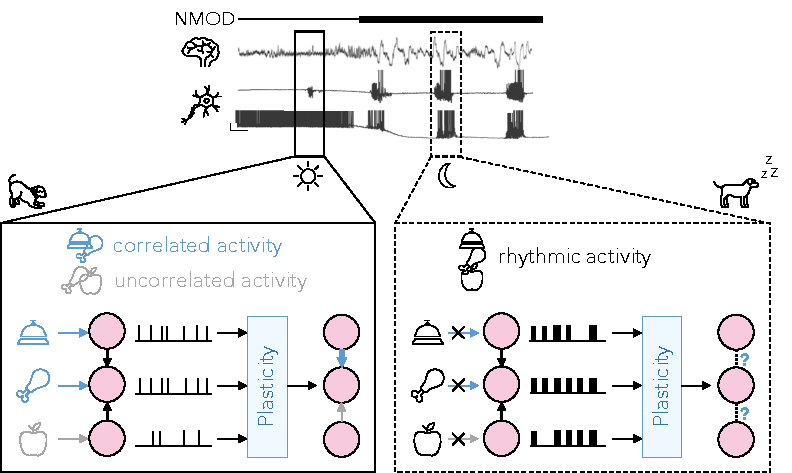
\includegraphics{fig/Review/fig_intro.pdf}
    \caption{\textbf{The impact of switches in brain states, neuronal activity onto synaptic plasticity remains unclear.} (Top) Switches in brain states (recorded by EEG signal) reflecting switches in neuronal firing activity are orchestrated by neuromodulators  (adapted from \cite{zagha_neural_2014}). (Bottom-left) During tonic firing associated to an active state, correlated neurons (bell-chicken) increase their synaptic weights while uncorrelated neurons (chicken-appel) decrease the weights. (Bottom-right) During synchronized bursting associated to a quiet state, external inputs are disconnected, neurons are bursting; synaptic change is not yet elucidated.  }
    \label{fig:intro}
\end{figure}



%%%%%%%%%%%%%%%%%%
vestiges de la review: \\
\begin{comment}
\textcolor{orange}{Je pense qu'on peut enlever ce paragraphe: c'etait pour indiquer comme c'etait compliqué de fitter le calcium car on n'a pas accès à des données clairement quantifiées}\\
\color{gray}
It is also important to not that fitting a calcium-dependent synaptic rule is challenging. Indeed,  recording internal calcium measure is complex. It requires fluorescent data from experiments. In addition to build a model based biological calcium amplitude and time-evolution,  lot of plasticity induction protocols exist such as:  \citep{yang_selective_1999, sjostrom_rate_2001, sjostrom_cooperative_2006, wittenberg_malleability_2006, nevian_spine_2006, letzkus_learning_2006, wang_coactivation_2005, paille_gabaergic_2013, fino_distinct_2010, frey_synaptic_1997, dudek_homosynaptic_1992, artola_different_1990, oconnor_dissection_2005, bloodgood_nonlinear_2007, bi_synaptic_1998, nishiyama_calcium_2000, froemke_spike-timing-dependent_2002, neveu_postsynaptic_1996, regehr_calcium_1992, yoshida_calcium_2001, sabatini_life_2002, ngo-anh_sk_2005,straub_how_2014}.
\color{black}
\end{comment}



%%%%%%%%%%%%%%ù%%
\subsection{Taxonomy: transversal analysis }
These excel sheets reveal several aspects of the state in the modeling of synaptic plasticity rules. First, the diversity in the implementation is very rich. There is no unique procedure to associate one given neuron model with one given rule. Nevertheless, some common practices appears such conductance-based models are mainly used in calcium-based modeling with a focus on the postsynaptic cell. It emphasizes that biophysical rules are study nowadays to explore and understand the mechanisms underlying synaptic plasticity. In order to unravel plasticity secrets, using more detailed rules is favorable. They are checked on experimental protocols. One makes sure that they fit experimental data to draw information on the functioning. 

On the other side, phenomenological rules are mostly used with integrate-and-fire neuron models in large network. Therefore, these rules are employed as a tool to study memory formation or consolidation. It is interesting to point out that phenomenological rules were first derived to match experimental curve. For example, STDP rule is the exponential fitting of the spike-time plasticity-induction protocol done 25 years ago. Now this rule is used to explore learning and memory. In addition, the association between integrate-and-fire neurons in large networks with phenomenological rules permits to save computation time. By contrast, conductance-based models with calcium-based rule require more differential equations implying longer time simulations.

Recently, the tendency in the field is to combine several synaptic plasticity rules and be the most creative. The synaptic plasticity rule will be developed to match a particular application or will be modified to infer the desired outcome. It rises the flag about the limitations of current synaptic rules or it might open the way to a multitude of new models (...) \textcolor{red}{j'aimerais bien mettre en avant le fait que le modèle de HH nous a bien aidé il y a 70 ans que depuis ce modèle on l'a modifié pour reproduire pleins d'activités neuronales, que les paramètres n'ont plus vraiment de "sens" et ca reste un très bon modèle pour montrer ce que l'on veut ... peut etre que pour la plasticité on devrait accepter cela et arreter de chercher une "unified" synaptic plasticity rule ... }\\
~\\
\textcolor{orange}{citer \cite{artola_long-term_1993} }



% ---------------------------------------------
% ---------------------------------------------
%
%       Different implementations but not really 
%
% ---------------------------------------------
% ---------------------------------------------
\section{Part III - Synaptic plasticity rules: different implementations but not really}

\subsection{Plasticity-induction protocols used to fit synaptic plasticity rules}
\textcolor{red}{....... l'explication des protocols est donné dans l'intro ....}

For phenomenological and biophysical synaptic rules, parameters are often fitted to reproduce one of these protocols. Figure \ref{fig:ProtocolRecap}B is thought-provoking because to reproduce two different plasticity-induced protocols (the frequency and the spike-time), two different sets of parameters are required. On one side, it can make sense to have two sets since these two protocols were obtained in two different areas (respectively the cortex and the hippocampus). This modeling practise is also observed in conductance-based neuron model when conductance values are adapted depending on the region. On the other side, it rises the question that for each region or each neuron type, the parameters need to be accurately fine-tuned. Compared to our analogy for conductance-based neuron model, a neuron of one given region can see its ion channel quantities vary in large interval and still generating the desired activity \citep{prinz_similar_2004}. 
\textcolor{orange}{j'essaye de faire un paralélisme sur la fragilité des modèles SP alors que les neurones sont hyper maléables cf  eve - je peux essayer de faire une analogie avec le fait qu'on essaye d'utiliser une "moyenne" mais que ce n'est pas biologogiquement plausible}.

Figure \ref{fig:ProtocolRecap}C illustrates a model during a spike-time dependent protocol at 50Hz, (top) using the parameter set fitted for the frequency protocol and (bottom) using the parameter set for the spike-time protocol.

It also triggers a flag that models are fitted at in-vivo deterministic very low firing spike but neurons are able to swipe from low frequency to high frequency \citep{cui_robustness_2018}. 


 \begin{figure}[H]
\centering
    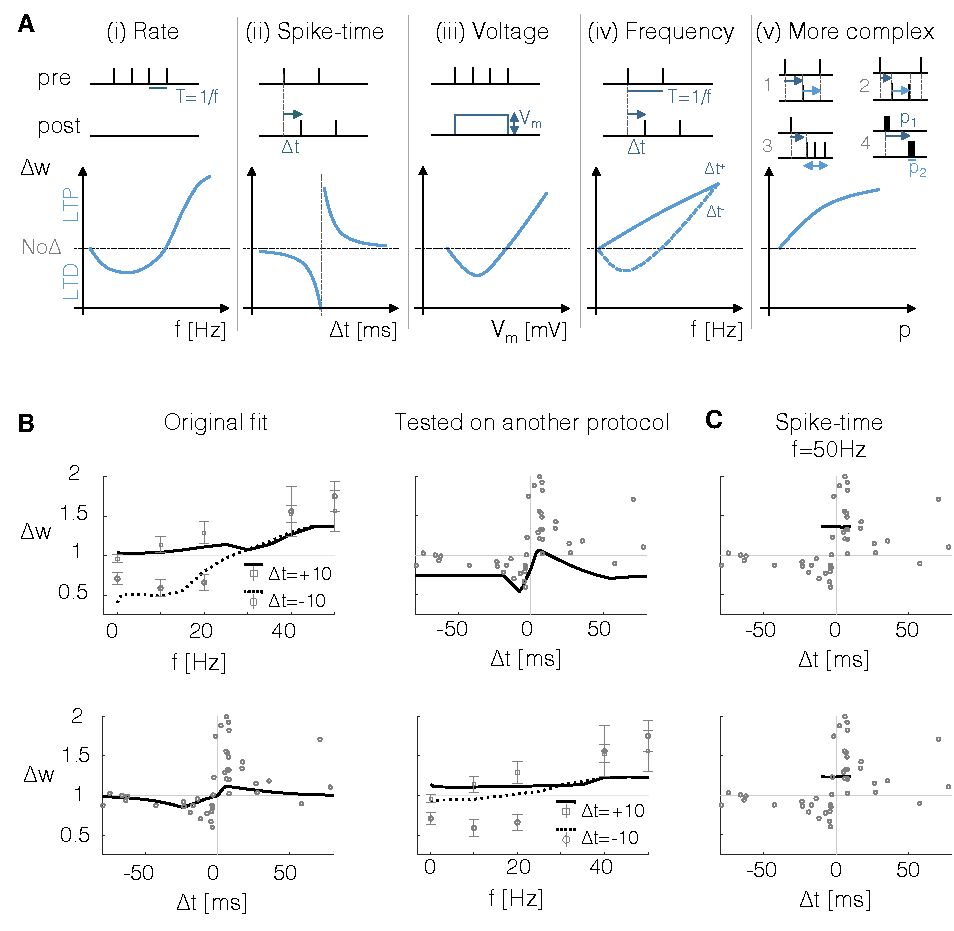
\includegraphics{fig/Review/Protocols.pdf}
    \caption{\textbf{Fitting of synaptic palsticity rules.} \textbf{A.} \textit{Experimental plasticity induction protocols are numerous.} (Top) The pre-post spiking activity is externally stimulated with a control parameter and a tested parameter. (Bottom) The evolution of the synaptic change ($\Delta w$) as function of the tested parameter. LTP and LTD refer to long-term potentiation and long-term depression. Rate protocol: the presynaptic neuron is spiking at a varying frequency $f$ \citep{dudek_homosynaptic_1992,bliss_long-lasting_1973}. (ii) Spike-time dependent plasticity: the presynaptic and postsynaptic neuron are both spiking at a given frequency (often 1Hz) with a changing delay $\Delta t$ between them \citep{bi_synaptic_1998} . (iii) Voltage: the presynaptic neuron is spiking and the postsynaptic is depolarized at a changing voltage membrane $V_m$ \citep{artola_different_1990, sjostrom_rate_2001}. (iv) Frequency-dependent induction protocol: both neurons are spiking at a frequency $f$. The presynaptic are preceding the postsynaptic spikes by $\Delta t^+=10$ms (or in the other way, post-pre $\Delta t^-=-10$ms \citep{sjostrom_rate_2001}. More complex protocols: others induction protocols using diverse tested parameters $p$. 1. Triplet: the time delay between the pre-post-pre is considered. 2. Quadruplet: the time delay between pre-post-post-pre. 3. Several postsynaptic spikes after a certain delay, the parameters are the number of spikes or the spiking frequency. 4. Bursting protocols: the burst duration and the burst delay are used to test the synaptic change. \textbf{B.} \textit{Synaptic rules fitted on one protocol cannot reproduce another protocol.} (top) The triplet model fitted on the frequency protocol (right) does not fit the spike-time protocol (left).  (bottom) The triplet model fitted on the spike-time protocol (right) does not fit the frequency protocol (left). Two parameter sets are required to fit the two different protocols. \textbf{C.} At 50Hz, whatever the parameter sets, the synaptic weight is potentiating. }
    \label{fig:ProtocolRecap}
\end{figure}


\subsection{To be (connected) or not to be}
Synaptic plasticity rules provide equations to describe one common goal: a definition for synaptic change. They are constrained by the same experimental \textit{in vitro}/in-vivo data. Since many years, theoreticians argue to show the relationships or the discrepancy between the different rules. 
 
For phenomenological models of plasticity, relationships are found in spite of their different implementations. Triplet model is an amelioration of the classical pair-based model to match a wider variety of experimental protocols \citep{pfister_triplets_2006}. It has been shown that it can also be mapped to rate-based learning rule as the BCM \citep{gjorgjieva_triplet_2011}. The sliding threshold of \citep{bienenstock_theory_1982} theory is also derived by introducing metaplasticity and other time-scales in the model \citep{el_boustani_stable_2012}.
Voltage-based model is actually an extension of triplet model \citep{clopath_connectivity_2010}. Heterosynaptic plasticity is reproduced by using a STDP rule combined with metaplasticity \citep{benuskova_stdp_2007}.

Similar mappings are shown in calcium-based rules. As mentioned in section XX, calcium-based rules are either described by a two-thresholds calcium function \citep{graupner_natural_2016} or a sigmoid calcium function \citep{shouval_converging_2002}. However, the two formulations are identical and they can be expressed by a generic model: $\tau([Ca]) \dot{w} = \Omega([Ca]) - w$ where $\tau([Ca])$ is the calcium-dependent time constant, $\Omega([Ca])$ is the calcium-dependent steady-state value. The coefficient identification is done in \citep{jacquerie_switches_2022}.

Then, phenomenological and biophysical models are often compared as shown in \citep{yeung_selectivity_2003, graupner_natural_2016, graupner_natural_2016, babadi_stability_2016}. 

\subsection{The apple does not fall far from the tree ?}
\textcolor{gray}{Je peux essayer de faire une sorte de petite arbre généalogique: Claudia Clopath a travaillé longtemps avec Wulfram Gerstner. Pfister est également un "enfant" de Gerstner. Rossum il a travaillé avec Gina turrigano (...) }


 
% ---------------------------------------------
% ---------------------------------------------
%
%       SMALL COMPUTATIONAL EXPERIMENTS 
%   TO SHOW INCOMPATIBILITY BETWEEN VAR & SP 
%
% ---------------------------------------------
% ---------------------------------------------
\section{Part IV - Incompatibility between synaptic plasticity rules, neuromodulation and biological variability}


% ---------------------------------------------
%                   experience 1
% ---------------------------------------------
\subsection{Synchronous bursting is not synchronous tonic}
Synaptic plasticity has been commonly studied in very stereotyped spiking protocol (see \textcolor{gray}{Figure Protocol}). For example, Spike-timing-dependent plasticity (STDP) relies on the exact spike timing between a presynaptic neuron and a postsynaptic neuron, driving either potentiation or depression \citep{bi_synaptic_1998}. Plasticity rules are fitted on such protocols and are able to reproduce synaptic changes acquired experimentally in spiking activity (see Figure \ref{fig:synchr}, tonic activity). However, neurons \textit{in vivo}  are not spiking as regularly as in these control conditions. Here we challenge the robustness of the plasticity rules during bursting activity where the emphasis is not focused on the spike-time itself but rather on the synchronicity of the whole rhythmic activity. To do so, we perform a simple computational experiment using a neuron circuit capable of switching between asynchronous spiking and rhythmic bursting states \citep{jacquerie_robust_2021, jacquerie_switches_2022}. Using a conductance-based modeling paradigm, the circuit reproduces the activities observed in cortical networks during switches in brain states \citep{mccormick_sleep_1997, zagha_neural_2014,chrol-cannon_computational_2014} among others. An inhibitory neuron projects GABA currents onto two excitatory neurons connected by an AMPA current (Figure \ref{fig:synchr}, right. See \nameref{sec: methods} for details). The synaptic strength between the two neurons is affected by synaptic plasticity, modeled either by a biophysical rule (two-threshold calcium levels established by \citep{graupner_natural_2016}) or a phenomenological rule (triplet rule from \citep{pfister_triplets_2006}). The circuit is able to switch from tonic to burst. This transition is driven by neuromodulators. These signaling substances are capable of changing the circuit state \citep{marder_neuromodulation_2014}. Neuromodulators are dynamically regulated, \textit{i.e.} their quantity is fluctuating across time. Even for one given brain state, variability in the concentration is observed. Here, we induced a small fluctuation of 5$\%$ during the burst rhythms. The endogenous burst remains similar with the qualitatively same intraburst frequency and duty cycle.  However, the evolution of the synatic weight computed by the two models lead to distinct behaviours. Indeed,  the phenomenological model is very sensitive to this small change in neuromodulator level, barely visible to the naked eyes (see Figure~\ref{fig:synchr}, bottom trace). The spike times are slightly shifted from mainly pre-post pattern inducing potentiation to post-pre pattern inducing depression (see zoom in Figure \ref{fig:synchr}) impacting drastically the time evolution of the weight. By contrast, biophysical models are blind to this perturbation. The calcium dynamic is driven by the burst itself and not the relative spike time inside the burst. The phenomenological rules are not adapted to capture plasticity in more complex firing activity \citep{gjorgjieva_burst-time-dependent_2009, jacquerie_switches_2022}.



\begin{figure}[H]
    \centering
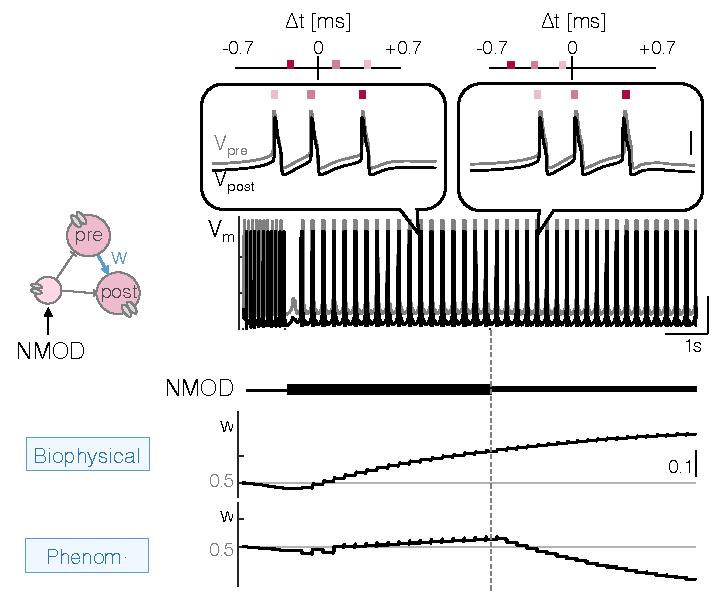
\includegraphics[scale=1]{fig/Review/fig_part3_synchr.pdf}
    \caption{\textbf{Phenomenological rules are sensitive to the relative spike times within an endogenous burst rhythm.} A 3-cell circuit composed of an inhibitory neuron connected to two excitatory neurons that have a plastic connection. Each neuron is a conductance-based model.
    Two seemingly similar patterns driven by slightly different neuromodulator levels (change in black bar size) lead to a slight difference on the pre-post pairing (pink squares on $\Delta t$). It results in an opposite synaptic weight change for phenomenological models (phenom.). On the contrary, biophysical model is blind to the change in neuromodulator level. (yscale-zoom: 50mV, time window-zoom: 90ms, voltage yscale: 50mV, , gray and black voltage traces are respectively the pre and postynaptic neuron activity).}
    \label{fig:synchr}
\end{figure}

% ---------------------------------------------
%                   experience 2
% ---------------------------------------------
\subsection{All synaptic plasticity rules are not suitable to handle intrinsic variability}
Neurons are highly variable in types, shapes, and even within the same category of neurons, intrinsic parameters are vastly different \citep{marder_multiple_2011}. Similar circuit activities can result from a large set of intrinsic conductances. These conductances are also ongoing turnover or they are under the control of neuromodulators. Here, we challenge the compatibility between synaptic plasticity rules and intrinsic variability. We use the same circuit in asynchronous spiking activity. Two intrinsic conductances are modified by 25$\%$ to 50$\%$. The activity is not perturbed but the evolution of the synaptic weight is different between the biophysical and the phenomenological rules (see Figure \ref{fig:intrinsic}). This difference in robustness comes from the driving mechanisms of the synaptic rule. For phenomenological models, the spike time is blind to change in intrinsic parameters. By contrast, the biophysical models are translating the calcium fluctuations into synaptic weight change. The intrinsic variability affects the calcium ion channels resulting in a change of intracellular calcium concentration, drastically impacting the evolution of the synaptic weight. It raises the controversy such tat two circuits with a similar activity but different sets of ion channels are supposed to have the same synaptic change (as seen in phenomenological rules) or these intrinsic differences drive different behavior in the synaptic connection. 


\begin{figure}[H]
    \centering
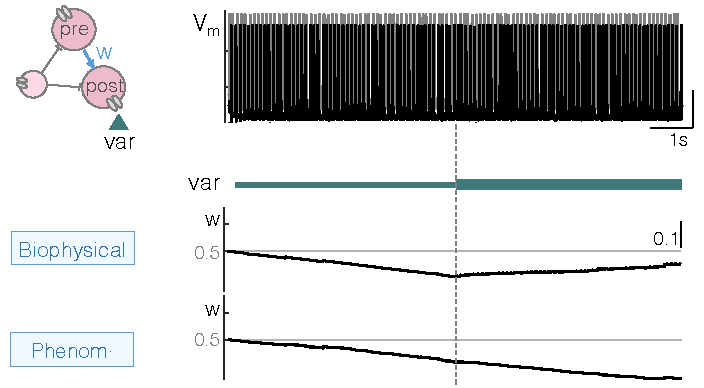
\includegraphics[scale=1]{fig/Review/fig_part3_intrinsic.pdf}
    \caption{\textbf{Change in intrinsic parameters affects the outcome of the biophysical models}. A 3-cell circuit composed of an inhibitory neuron projecting to two excitatory neurons whom synaptic strength is plastic. Each neuron is a conductance-based model. The circuit is in asynchronous spiking regime. As soon as the postsynaptic neuron conductance is affected by variability (var) mimicking the effect of neuromodulator, the outcome of the biophysical rule is affected. The phenomenological rule (Phenom.) is blind since the spiking activity is not modified. (Voltage scale: 50mV, gray and black voltage traces are respectively the pre and postynaptic neuron activity) }
    \label{fig:intrinsic}
\end{figure}

% ---------------------------------------------
% ---------------------------------------------
%
%               Conclusions Review
%
% ---------------------------------------------
% ---------------------------------------------
\subsection{Conclusion and perspectives}
\color{gray}
- J'aimerais bien orienter la conclusion en expliquant un peu comme eve marder que ce n'est pas forcément la moyenne des résultats de plasticité qui va donner une loi uniforme qui va fonctionner pour tous les modèles. 
Que c'est un peu comme reproduire une activité électrique d'un neurone, il y a pleins de combinaisons possibles de paramètres qui va fonctionner. Que ces règles sont aussi capabables de s'adapter via les neuromodulateurs pour respecter le fonctionnement du neurone. Mais le probleme dans la litérature actuelle c'est qu'on essaye de tuner les règles soit pour reproduire parfaitement des protocoles expérimentales qui sont très stéréotypés soit on construit des règles pour observer un phénomène d'apprentissage bien précis. - - - ca reste encore flou dans ma tête. 
- consider protocols with noise or more in vivo-like firing activity (example: \cite{cui_robustness_2018}).\\
- [Suvrathan, 2018] "In summary, coincidence-based rules for synaptic plasticity are no longer sufficient to explain the diversity of ways neural circuits can adapt and learn. The rules for plasticity can cover much longer timescales than previously thought and vary depending on the circuit they are embedded in, forcing both a reevaluation of the synaptic basis of learning rules as well as investigation into underlying mechanisms that can bridge long timescales"\\
- STDP in neural network (machine learning) >>  alors qu'on a montré que ce n'était pas robust 



\color{black}

\section{Methods}
\label{sec: methods}
Simulations were performed using the Julia programming language \cite{bezanson_julia_2017}. Data processing were performed either in Matlab. Code files are freely available at \url{https://github.com/KJacquerie/Review}.


\subsection{Neuron model and synaptic plasticity rules}
\label{sec: plasticity}
A 3-cell circuit was modeled using a conductance-based model. The neuronal model is the same used in \citep{jacquerie_switches_2022}. The inhibitory cell controls the rhythm of the circuit. An hyperpolarizing current applied to the inhibitory neuron switches the whole circuit in rhythmic bursting mode. This hyperpolarizing current models the effect of a neuromodulator signal (NMOD) \citep{zagha_neural_2014}. 

Regarding the plasticity between the pre- and postsynaptic cells, we used the triplet model defined in \citep{pfister_triplets_2006} for the phenomenological rule and the calcium-based model is defined in \citep{graupner_natural_2016}. More information is available \textcolor{gray}{SI Appendix or \citep{jacquerie_switches_2022}}.



\subsection{Computational experiments}

Figure \ref{fig:synchr} shows a neuronal switch from tonic to burst induced by neuromodulation with variable neuromodulator drive. Tonic activity is simulated by inducing spikes in the pre and postsynaptic cells with a strong current $I_{\mathrm{app}} = 50 \mathrm{nA}/\mathrm{cm^2}$ for a short duration of 3ms at a frequency of 10 $\mathrm{Hz}$ for 1s. The interspike intervals follow an independent Normal Distribution $\mathcal{N}(\frac{1}{f_0}, (\frac{\num{0.1}}{f_0})^{2})$, $f_0 = 10\mathrm{Hz}$. Then, A current $I_{\mathrm{app},\mathrm{I}} = -1.2 \mathrm{nA}/\mathrm{cm^2}$ is then applied to the inhibitory cell to mimic the impact of neuromodulators and induce bursting. After 6s, the applied current is changed to $I_{\mathrm{app},\mathrm{I}} = -1.\mathrm{nA}/\mathrm{cm^2}$. 

Plasticity is implemented between the pre- and postsynaptic neurons using the triplet and the calcium-based model mentioned above. The synaptic weight (w) evolution shows that both plasticity rules evolve the same in tonic mode according to the pairing protocol \citep{sjostrom_rate_2001}. However, the switch to burst induce divergent results between the two types of rules.\\

Figure \ref{fig:intrinsic} shows a tonic firing pattern with differences in the $g_{\mathrm{CaT}}$,  $g_{\mathrm{K,Ca}}$ conductances and affecting the postsynaptic calcium influx (more specially the parameter $C_{\mathrm{post}}$ in the calcium-based model \citep{graupner_natural_2016}). Spikes are generated by applying a strong current $I_{\mathrm{app}} = 50 \mathrm{nA}/\mathrm{cm^2}$ for a short duration of $3\mathrm{ms}$. The interspike intervals following independent Normal distributions $\mathcal{N}(\frac{1}{f_0}, (\frac{\num{0.1}}{f_0})^{2})$, $f_0 = 10\mathrm{Hz}$. From 0 to $5.5\mathrm{s}$, conductances values are  $g_{\mathrm{CaT}}=0.55$, $g_{\mathrm{K,Ca}}=4$, $C_{\mathrm{Post}}=1.62138$. Then, $g_{\mathrm{CaT}}=0.55\cdot1.5$, $g_{\mathrm{K,Ca}}=4\cdot0.75$, $C_{\mathrm{Post}}=1.62138\cdot 1.5$.




%-------------- Reset 
%\chapter{Homeostatic reset}
\section{Introduction}
\section{Methods and Computational experiments}
\section{Results}
\section{Discussion}


%-------------- Memory Task
%\chapter{Memory consolidation through combined burst-induced homeostatic reset and structural plasticity}
\begin{shaded}
BLA BLA

\end{shaded}

% -------------------------------
% -------------------------------
%
%        INTRODUCTION
%
% -------------------------------
% -------------------------------
\section{Introduction}
\textcolor{blue}{OCNS}\\
Neurons adapt their connections with each other through synaptic plasticity, driven by correlations in their spiking activity (Fig. 1A). Additionally, neuronal networks undergo global changes in rhythmic activity that correspond to different brain states, defined by switches in neuronal activity and orchestrated by neuromodulators. A well-known example is the transition from a state of learning during active waking to rest during quiet waking, which corresponds to a switch in neuronal activity from tonic firing to bursting (Fig. 1B). This raises the question of how switching from tonic firing to bursting affects the outcome of synaptic plasticity and whether it can support memory consolidation.
Recently, we have shown for a variety of synaptic plasticity models that bursting leads to a homeostatic reset, in which synaptic efficacy returns to a fixed baseline value irrespective of the starting point. This homeostatic reset causes the network to forget any learned information [1]. To address this issue, we propose an additional structural plasticity mechanism in which short-term changes in synaptic efficacy – evolving according to traditional plasticity rules – drive long-lasting morphological changes such as spine growth or insertion of new AMPA receptors. While synaptic efficacy undergoes homeostatic reset during bursting, information is consolidated through structural plasticity on a longer timescale.
We demonstrate the utility of this mechanism in a network of neurons using a conductance-based neuronal model that can switch from tonic firing to bursting along with a calcium-based synaptic rule to drive changes in synaptic efficacy. We investigate three regimes of switches in neuronal activity and plasticity mechanisms, denoted S1, S2, S3 (Fig. 1C). In S1, as a control condition, tonic firing is interleaved with periods of neuronal inactivity – mimicking bursting blockers – and a traditional plasticity rule, while in S2, tonic firing is separated by periods of bursting, leading to homeostatic reset in synaptic efficacy. Configuration S3 is identical as S2 but also includes our proposed burst-driven structural plasticity. 
In our first memory task (Fig. 1D), we show that the signal-to-noise (SNR) is improved over repeated switches only in S3. In a simple pattern recognition task (Fig. 1E), blocking bursting activity (S1) makes the network fragile to noise, and blocking structural plasticity during bursting leads to complete forgetting (S2), neither of which occurs in S3. Finally, in a MNIST recognition task (Fig. 1F), we confirm that memory consolidation occurs with S3 by showing a stronger receptive field that consolidates during switches from tonic to burst and is robust to noise. 
In this work, we shed light on the under-investigated role of switches in neuronal firing patterns for synaptic plasticity. Traditional plasticity rules result in a burst-induced homeostatic reset of synaptic efficacy, which is incompatible with memory consolidation. Our burst-driven structural plasticity proposes a solution to this problem, bridging the gap between switches in tonic firing to bursting, learning, and memory consolidation, and suggesting new ways to improve machine learning algorithms. 




% -------------------------------
% -------------------------------
%
%           METHODS
%
% -------------------------------
% -------------------------------

\section{Methods and Computational experiments}
\subsection{Conductance-based modeling}
\textcolor{blue}{same as reset}\\
\textcolor{orange}{est-ce que je le renote ici brèvement}

\subsection{Circuit architecture}
\textcolor{red}{parler du courant syn ou le mettre direct dans conductance-based modeling}
% -------------------------------
%     Traditional plasticity
% -------------------------------
\subsection{Synaptic plasticity}
\subsubsection{Definition of the synaptic strength}
The synaptic current between the excitatory presynaptic neuron and postsynaptic neuron is an AMPA current as $I_\mathrm{syn} = I_\mathrm{AMPA}$, defined by $I_\mathrm{AMPA} = wg s_\mathrm{AMPA}(V_\mathrm{m}-E_\mathrm{AMPA}$. The synapse is modeled by $wg$ called the effective synaptic weight where $w$ the  \textit{synaptic efficacy}, and $g$ is the \textit{synaptic conductance}. The variable $w$ is driven by traditional synaptic plasticity rules. We compared the pair-based rule \citep{abbott_synaptic_2000} or the calcium-based plasticity rule \citep{graupner_natural_2016} \textcolor{magenta}{check for triplet?}. The variable $g$ is governed by a structural plasticity rule developed in this project (explained in the following section).

\subsubsection{Calcium-based model}
\textcolor{blue}{la meme regle clacique que dans le reset}\\
\textcolor{orange}{est-ce que je le note}
\subsubsection{Pair-based model}
idem

% -------------------------------
%           Methods: structural plasticity
% -------------------------------

\subsubsection{Structural plasticity: plasticity on the synaptic conductance $g$}

The Late phase of Long-term plasticity relie on the generation of de novo proteins and morphological changes. These changes are encapsulated in a variable $g$, for simplicity called the synaptic conductance. The rule governing the change in this variable refers to structural plasticity. We developed a simple equation driven by the \textit{ homeostatic reset}, which is the result of the soft-bound traditional plasticity rule acting on $w$ during burst \citep{jacquerie_switches_2022}.  
This simple equation is written as
$$ \tau_g \dot{g} = \Delta g $$
where $\Delta g$ is comprised between -1 and 1 and decides if the conductance increases (positive value of $\Delta g$) or decreases (negative value of $\Delta g$). The term $\tau_g$ scales the speed of change is in order of magnitude of 1 to 10 seconds (\textcolor{blue}{add the exact value for each experiment in \textit{SI Appendix})}.


\textit{During bursting activity only}, the variable $\Delta g$ has the following dynamics: 
$$ \tau_\Delta \dot{\Delta g} = f(w) - \Delta g$$
where $\tau_\Delta$ is the time constant associated to the change in $\Delta g$ and $f(w)$ is a sigmoidal function between -1 and 1 written as:
$$ f(w) = -1+2\left( \frac{e^{\mathrm{slope} (w-w_\mathrm{HR})}}{1+e^{\mathrm{slope} (w-w_\mathrm{HR})}} \right) $$
where slope defines the steepness of the sigmoid (the largest the value, the steepest the transition from -1 to 1). The term $w_\mathrm{HR}$ is the homeostatic reset estimated each second during the bursting activity. 

For the calcium-based rule, the estimated reset value is computed by 
\begin{align}  w_\mathrm{HR} 
    & = \frac{ \Omega^\mathrm{d}\alpha^\mathrm{d} +\Omega^\mathrm{p}\alpha^\mathrm{p} }{\alpha^\mathrm{d} + \alpha^\mathrm{p}}.
\end{align}
where $\Omega^\mathrm{d}$ and $ \Omega^\mathrm{p}$ are respectively the depression and potentiation levels and the effective time spent in each region $\alpha^\mathrm{d}$ and $\alpha^\mathrm{p}$ are defined as the time spent balanced by the time-constant of potentiation/depression in the corresponding region (as demonstrated in \citep{jacquerie_switches_2022}).
~\\
~\\
\textcolor{magenta}{decide if we repeat the experiment for the phenomenological rule}\\
\color{gray}
For the pair-based rule, the estimated reset value is given by 
\[ w_\mathrm{HR} = \frac{\frac{A^+C^+}{A^-C^-}}{1+\frac{A^+C^+}{A^-C^-}}.\]
with $A^+$ and $A^-$ are the potentiation and depression parameters of the pair-based rule. $C^+$ is the average correlation value between pre- and post- spiking time trains and $C^-$ is the average value between the post- and pre- spiking time trains (as demonstrated in \citep{jacquerie_switches_2022}). 
\color{black}


The bursting rhythm dictates the value of the homeostatic reset. Since it can be influenced during the state for example by neuromodulators or connectivity increase, the estimated value of the reset is computed each second which is realistic as the interburst frequency is around \textcolor{magenta}{add the value}.

If the neuron is not bursting, $\tau_\Delta \dot{\Delta g} = -\Delta g$. This value is converging towards 0. It guarantees the conductance to remain unchanged during the other states - an assumption made in this project. 

\subsubsection{Regimes}
Table \ref{tab:SP_overview} summarizes the different combinations between the switches between the different firing patterns (tonic firing, inactive, burst) and the different synaptic plasticity rules. 

\begin{table}[h]
    \centering
    \begin{tabular}{l|l|l|l|l}
        Model     & bounds & $\dot{w}$  & $\dot{g}$ & switch\\
        \hline
         $\#$1   & soft &  $\tau_w \dot{w} = \Omega([\mathrm{Ca}]) -w$ & fixed value   & tonic-inactive\\
         $\#$2   & soft &  $\tau_w \dot{w} = \Omega([\mathrm{Ca}]) -w$ & fixed value   & tonic-burst\\
         $\#$3  & soft &  $\tau_w \dot{w} = \Omega([\mathrm{Ca}]) -w$ & $\tau_g \dot{g} = \Delta g$ & tonic-burst   \\
         $\#$4  & hard &  $\tau_w \dot{w} = \Omega([\mathrm{Ca}])$ & fixed value  & tonic-inactive  \\
         $\#$5 &hard &  $\tau_w \dot{w} = \Omega([\mathrm{Ca}])$ & fixed value  & tonic-burst  \\
    \end{tabular}
    \caption{Overview of the synaptic plasticity models}
    \label{tab:SP_overview}
\end{table}




% -------------------------------
%           Methods: computational expm
% -------------------------------
\subsection*{Computational experiments}
\label{sec:computaional_expm}


% - - - - - - - - - - - - - - - - - 
%           comp expm: Gonz
% - - - - - - - - - - - - - - - - - 
\subsubsection{Pairing neurons}
\textit{Network}\\
We reproduce a similar computational experiment as in \citep{gonzalez-rueda_activity-dependent_2018}. We build a 2-layer network with 100 input neurons connected to one output neuron. An inhibtory neuron is connected via GABA\textsubscript{A} and GABA\textsubscript{B} currents to all the excitatory neurons with a fixed connectivity.\\
~\\
\textit{Simulations of the different states}\\
The network has three possible states: tonic firing, bursting, inactive.
\begin{itemize}
\item[-] During the tonic-firing learning state, we pair 5 of the 100 presynaptic neurons with the postsynaptic neuron by driving them with correlated inputs. The active input neuron receives a depolarizing current of 50 nA/cm$^2$ during 3ms at a frequency of $f_0 = 60$ Hz. The output neuron receives a similar input at $f_0 =40 $ Hz \citep{gurunathan_spurious_2020}. This input is sufficient to generate an action potential in the conductance-based model. To build a more realistic simulation, the spike timings are generated with interspike intervals following independent Normal distributions $\mathcal{N}(\frac{1}{f_0}, (\frac{\num{0.1}}{f_0})^{2})$. The 95 non correlated input neurons are stimulated in the similar manner except that the frequency $f_0$ is chosen between the following values (0.1, 0.25, 0.5, 0.75, 1, 1.25, 1.5, 2) Hz  from a uniform distribution. The output neuron is stimulated with a pulse train at 40Hz whose interspike intervals follow independent Normal distribution $\mathcal{N}(\frac{1}{f_0}, (\frac{\num{0.1}}{f_0})^{2})$.
\item[-] During bursting, the inhibitory cell is hyperpolarized with an external applied current equal to -1.2 nA/cm$^2$. 
\item[-] During inactive state, the neurons are driven with an applied current generating pulse at a frequency $f_0$ chosen in the range (0.1, 0.5, 1) Hz.   The spike timings are generated in the same manner following independent Normal distributions  $\mathcal{N}(\frac{1}{f_0}, (\frac{\num{0.1}}{f_0})^{2})$. 
\end{itemize}
\textcolor{red}{in Appendix SI -- } provide a table with the different value of the parameter used for the synaptic plasticity rules. \\
~\\
\textit{Protocols}\\
We record the evolution of the efficacy and the conductance during five cycles that is alternating between a tonic-firing learning state with either an intermittent bursting state or an inactive state without bursting. Each state lasts 15 seconds.

~\\
\textit{Analysis}\\
To analyse the evolution of the effective synaptic throughout the simulation, we compute the Signal-to-Noise Ratio (SNR) at the end of each state. The SNR is computed according to \citep{gonzalez-rueda_activity-dependent_2018}; $\mathrm{SNR} = \mathrm{max}(w)/\mathrm{mean}(w)$. \textcolor{red}{ce n'est pas wg ? }



% - - - - - - - - - - - - - - - - - 
%           comp expm: Gonz
% - - - - - - - - - - - - - - - - - 
\subsubsection{Pattern recognition}
\textcolor{red}{ref} \citep{fauth_self-organized_2019}, ...\\
In the pattern recognition task, we build a network of 9 presynaptic neurons connected to two postsynaptic neurons. The network learns to identify two patterns created in 3x3 pixel grid. Each pixel is associated to its own input neuron. An inhibtory neuron is connected via GABA\textsubscript{A} and GABA\textsubscript{B} currents to all the excitatory neurons with a fixed connectivity.\\
~\\
\textit{States}\\
The network can be in four different states: 
\begin{itemize}
    \item[-] learning state: inputs neurons are driven with an external current according to the pattern. If the pixel is active, the associated input neuron receives a applied current as a pulse at a frequency $f_0$ chosen in a normal distribution $\mathcal{N}(55$Hz$, 10)$. The amplitude of the pulse is equal to 50nA/cm$^2$ and the duration is equal to 3ms. To mimic a less regular spiking trains, the interspike interval is obtained in $\mathcal{N}(\frac{1}{f_0}, (\frac{\num{0.1}}{f_0})^{2})$. If the pixel is inactive, a similar stimulation is applied for a frequency $f_0$ chosen in a normal distribution $\mathcal{N}(1$Hz$, 0.01)$. The output neuron associated to the presented pattern is stimulated with a pulse train at $f_0$ = 40Hz whose interspike intervals follow independent Normal distribution $\mathcal{N}(\frac{1}{f_0}, (\frac{\num{0.1}}{f_0})^{2})$. The other neuron has a similar pulse train except that $f_0 = 0.01$Hz.  
    \item[-] bursting state: the inhibitory neuron is hyperpolarized by a current of -1.2nA/cm$^2$.
    \item[-] inactive state: all excitatory neurons are inactive and receive a pulse train at a frequency $f_0$ chosen in a normal distribution $\mathcal{N}(1$Hz$, 0.1)$.
    \item[-] noisy state: to mimic a noisy state, all neurons receive a pulse train at a frequency $f_0$ chosen in a normal distribution $\mathcal{N}(15$Hz$, 10)$. 
\end{itemize}
~\\
\textit{Protocols}\\
We build the following protocol in order to compare the different models with and without the structural plasticity rule and the effect of bursting state. The network sees 20 consecutive states. 
During the 12 first ones, learning state is interleaved by bursting state (for Models $\#$2, 3 and 5). The thirteenth state is the noisy state followed by a bursting state (for Models $\#$2, 3 and 5). The last part of the simulation is composed of succession between inactive states and bursting state (for Models $\#$2, 3 and 5). To study the impact of burst in the simulation, we reproduce the same protocol by replacing all the bursting states by resting states  (for Models $\#$ 1 and 4). 
During learning, we decide to either show one sample of the first pattern half of the state followed by one sample of the second pattern or we show two samples of the same pattern. Each state lasts 15s. \textcolor{red}{VERIFIER SI C'EST BIEN CA QUE JE FAIS ou plutot 1-3-4-7-9-10 pour pattern 1}. 
~\\
\textit{Testing}\\
The network has been simulated with the same protocol and the same samples for each synaptic plasticity models. To test their ability to recognize the two patterns, we create 50 samples of the first pattern and 50 samples of the second pattern. To build this sample, each active pixel (associated to the pattern) is firing according to a pulse train at a frequency $f_0$ chosen in a normal distribution $\mathcal{N}(65Hz,10)$. Each inactive pixel is stimulated in a similar manner at a frequency $f_0$ of $\mathcal{N}(2Hz,1.5)$.

Each pattern is shown 1s and we count the number of spikes of the two output neurons. We reproduce this process in the network with a fixed connectivity whose the value of $w$ and $g$ are retrieved from the simulation after each state. 

During testing, the output neurons are not stimulated. 

\textcolor{red}{ajouter la partie ou on ne teste que trois pixels sur 4}\\


\textcolor{magenta}{ajouter la partie ou on fait de l'overlap? }



~\\
\textit{Analysis}\\
description of prediction and certainty\\
\textcolor{red}{wait for the discussion with Dan - GD}\\
~\\
More details on all computational experiments can be found on \textit{SI Appendix}.


% - - - - - - - - - - - - - - - - - 
%           comp expm: MNIST
% - - - - - - - - - - - - - - - - - 
\subsubsection{MNIST}
\textit{Dataset/network}\\
~\\
\textit{States}\\
~\\
\textit{Protocols}\\
~\\
\textit{States}\\
~\\




% -------------------------------
% -------------------------------
%
%           RESULTS
%
% -------------------------------
% -------------------------------

\section{Results}
% -------------------------------
%           RESULT 1
% -------------------------------
\subsection{Structural plasticity prevents forgetting due to burst-induced homeostatic reset}

\textcolor{red}{ajouter la description pour les hard bounds}\\
As a simple testbed, we consider a circuit consisting of three biophysical conductance-based model neurons: an excitatory AMPA neuron (pre) synapsing onto another excitatory neuron (post), and an inhibitory GABA neuron synapsing onto both. Applying a hyperpolarizing current to the inhibitory cell models the effect of neuromodulators and switches the network state from tonic firing to bursting. The “post” neuron receives current from the “pre” neuron in proportion to the synaptic \textcolor{cyan}{conductance} $g$ (e.g. the number of AMPA receptors or the size of the dendritic spine) and synaptic \textit{efficacy} $w$ (e.g. the efficacy of AMPA receptors), such that the effective $synaptic weight$ is their product $wg$ (Fig. 1A). Traditional plasticity rules \citep{song_competitive_2000, graupner_natural_2016, pfister_triplets_2006} propose plasticity dynamics $\dot{w}$ to update the synaptic efficacy w and have been previously validated in this model on experimental data \citep{sjostrom_rate_2001, bi_synaptic_1998}. These traditional rules accurately explain change in synaptic efficacy $w$ that are independent on de novo protein synthesis, often referred as \textit{early phase Long Term Potentiation }(E-LTP) \citep{lamprecht_structural_2004}. 

To explore the interaction between synaptic plasticity and global brain states, we define three neuronal firing patterns; inactive , tonic firing (correlated or uncorrelated between pre and postsynaptic neurons for mimicking learning or not) or bursting (Fig. 1B). We simulate the network in a tonic state with a calcium-based plasticity driving change in synaptic efficacy \citep{graupner_natural_2016}. This state mimics a learning state by driving the excitatory neurons with either correlated or uncorrelated inputs (Fig. 1C, blue panels). As expected, strongly correlated neurons increase their efficacy (black curve), while weakly correlated ones have unchanged or decreased efficacy (Fig. 1C, gray curves). We then explore how learning is affected when tonic firing is followed by another firing pattern. In S1, when neurons switch from tonic firing to an inactive state, the weights remain unchanged. This illustrates a situation where bursting is blocked, for example in absence of external stimulus or in the presence of neuromodulator blockers (Fig. 1C, left). However, when switching from tonic firing to bursting (S2), homeostatic reset occurs, and the synaptic efficacy returns to its baseline, regardless of its learned value (Fig. 1C, center). This means that switching into a brain state driven by low-frequency oscillation, characterized by bursting activity at the neuronal level, erases all information previously stored in the synaptic efficacy value. This phenomenon was shown to be robust to intrinsic neuron variabilities, network heterogeneity and neuromodulation \citep{jacquerie_switches_2022}.


To address this issue with traditional plasticity rules on $\dot{w}$ and their limited ability to consolidate memory, we propose a mechanism of structural plasticity through dynamics in the synaptic conductance, $\dot{g}$, referred to \textit{late phase Long Term Potentiation} (L-LTP). This type of plasticity, which is protein-synthesis dependent, is associated with long term changes \citep{lamprecht_structural_2004, abraham_is_2019}. Although $w$ undergoes homeostatic reset as before, $g$ consolidates learned information. If the synaptic efficacy $w$ is higher than its reset value, the conductance $g$ increases through spine growth or insertion of new synthesized receptors (S3). Conversely, if $w$ is lower than its reset value, $g$ decreases through down-selection (Fig. 1C, right). Our work offers insights into the potential of incorporating structural plasticity during burst for improved memory consolidation, while the rest of the network weights return to baseline and are available for future learning. 


\begin{figure}
    \centering
    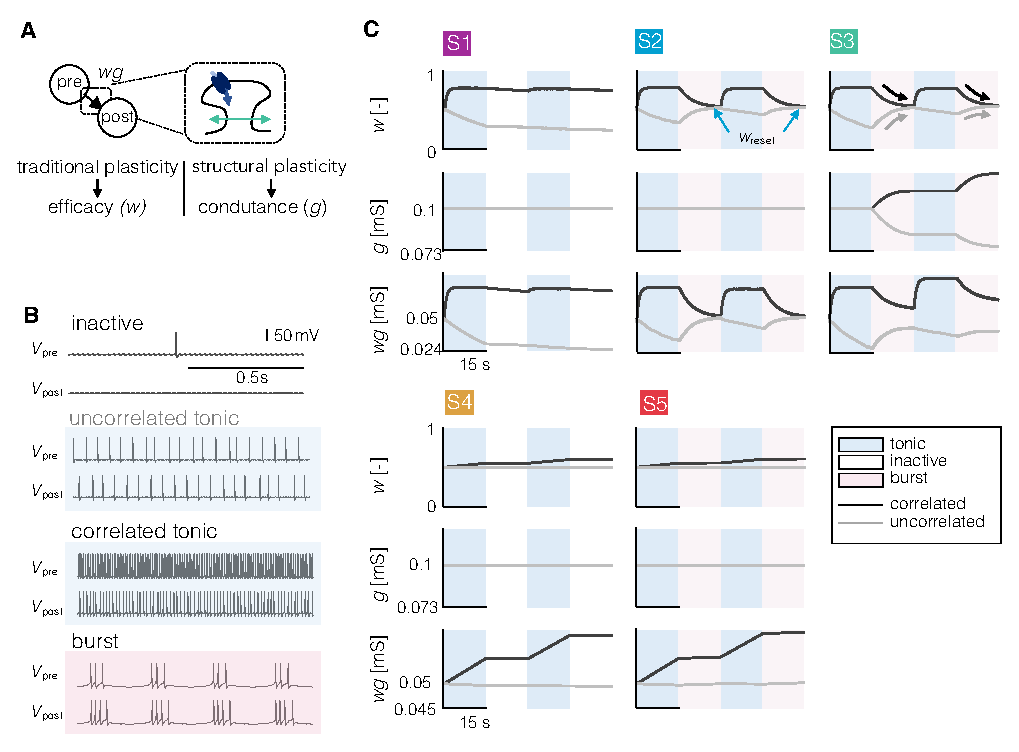
\includegraphics{fig/Task/Fig1.eps}
    \caption{Caption}
    \label{fig:Task_1}
\end{figure}


% -------------------------------
%           RESULT 2
% -------------------------------
%\subsection{Learning consolidates during burst through structural plasticity}
\subsection{Homeostatic reset and structural plasticity work together for memory consolidation}
We consider three memory tasks and compare the effect of different configurations of switches with their associated plasticity mechanisms. 

In the first memory task (Fig. 1D), as in \citep{gonzalez-rueda_activity-dependent_2018}, we pair five of 100 presynaptic neurons with a single postsynaptic neuron by driving them with correlated inputs in a tonic firing learning state. The remaining presynaptic neurons are uncorrelated. We repeated this procedure five times with either intermittent inactive states (S1) or bursting states (S2-S3). We find that only burst-driven structural plasticity paired with the homeostatic reset (S3) shows an increasing signal-to-noise (SNR) in the synaptic weights, over the course of multiple states. Suppressing bursting (S1) prevents the homeostatic reset but saturates the SNR at its steady-state value, while the calcium-based rule alone leads to forgetting through burst-induced homeostatic reset (S2). 



\begin{figure}
    \centering
    \includegraphics{fig/Task/Fig2.eps}
    \caption{Caption}
    \label{fig:Task_2}
\end{figure}


\begin{figure}
    \centering
    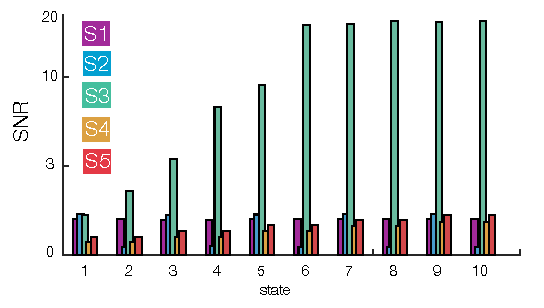
\includegraphics{fig/Task/Fig2_bar}
    \caption{Caption}
    \label{fig:Task_2_bar}
\end{figure}


% ---------------------------------------
%       RESULT 3: Pattern 
% ---------------------------------------
In the second memory task, we design a pattern recognition task (Fig. 1E), in which the network learns to identify two patterns, A and B. Each pixel of the grid is associated to one input neuron \citep{gurunathan_spurious_2020}. To emulate a variety of patterns, an input neuron which is associated to a pixel belonging to the pattern is tonically firing around 55Hz, while the other pixels are firing around 1Hz. During the tonic firing learning state, each pattern is paired with a corresponding output neuron. Learning states are interleaved with either inactive (S1) or bursting states (S2-S3) as in the first task. To test the robustness of the network to interference, we also add a noisy state in which neurons are tonically firing around 15Hz. During testing, we present either pattern A or B, which should cause only the corresponding output neuron to fire. The performance is computed after each state switch, and corresponds to the percentage of recognized patterns. We see that the burst-driven structural plasticity rule paired with the homeostatic reset (S3) allows memory consolidation and shows improved robustness to noise compared to the two other cases (S1-S2). In S1, the network, which illustrates the interaction between switches in tonic firing and a traditional synaptic plasticity rule alone, entirely forgets any learning as soon as noisy patterns are shown. In S2, once again we observe that each bursting state resets any learning. 

\textcolor{red}{ajouter la partie overlap ? et reconnaissance 3 digits? }


\begin{figure}
    \centering
    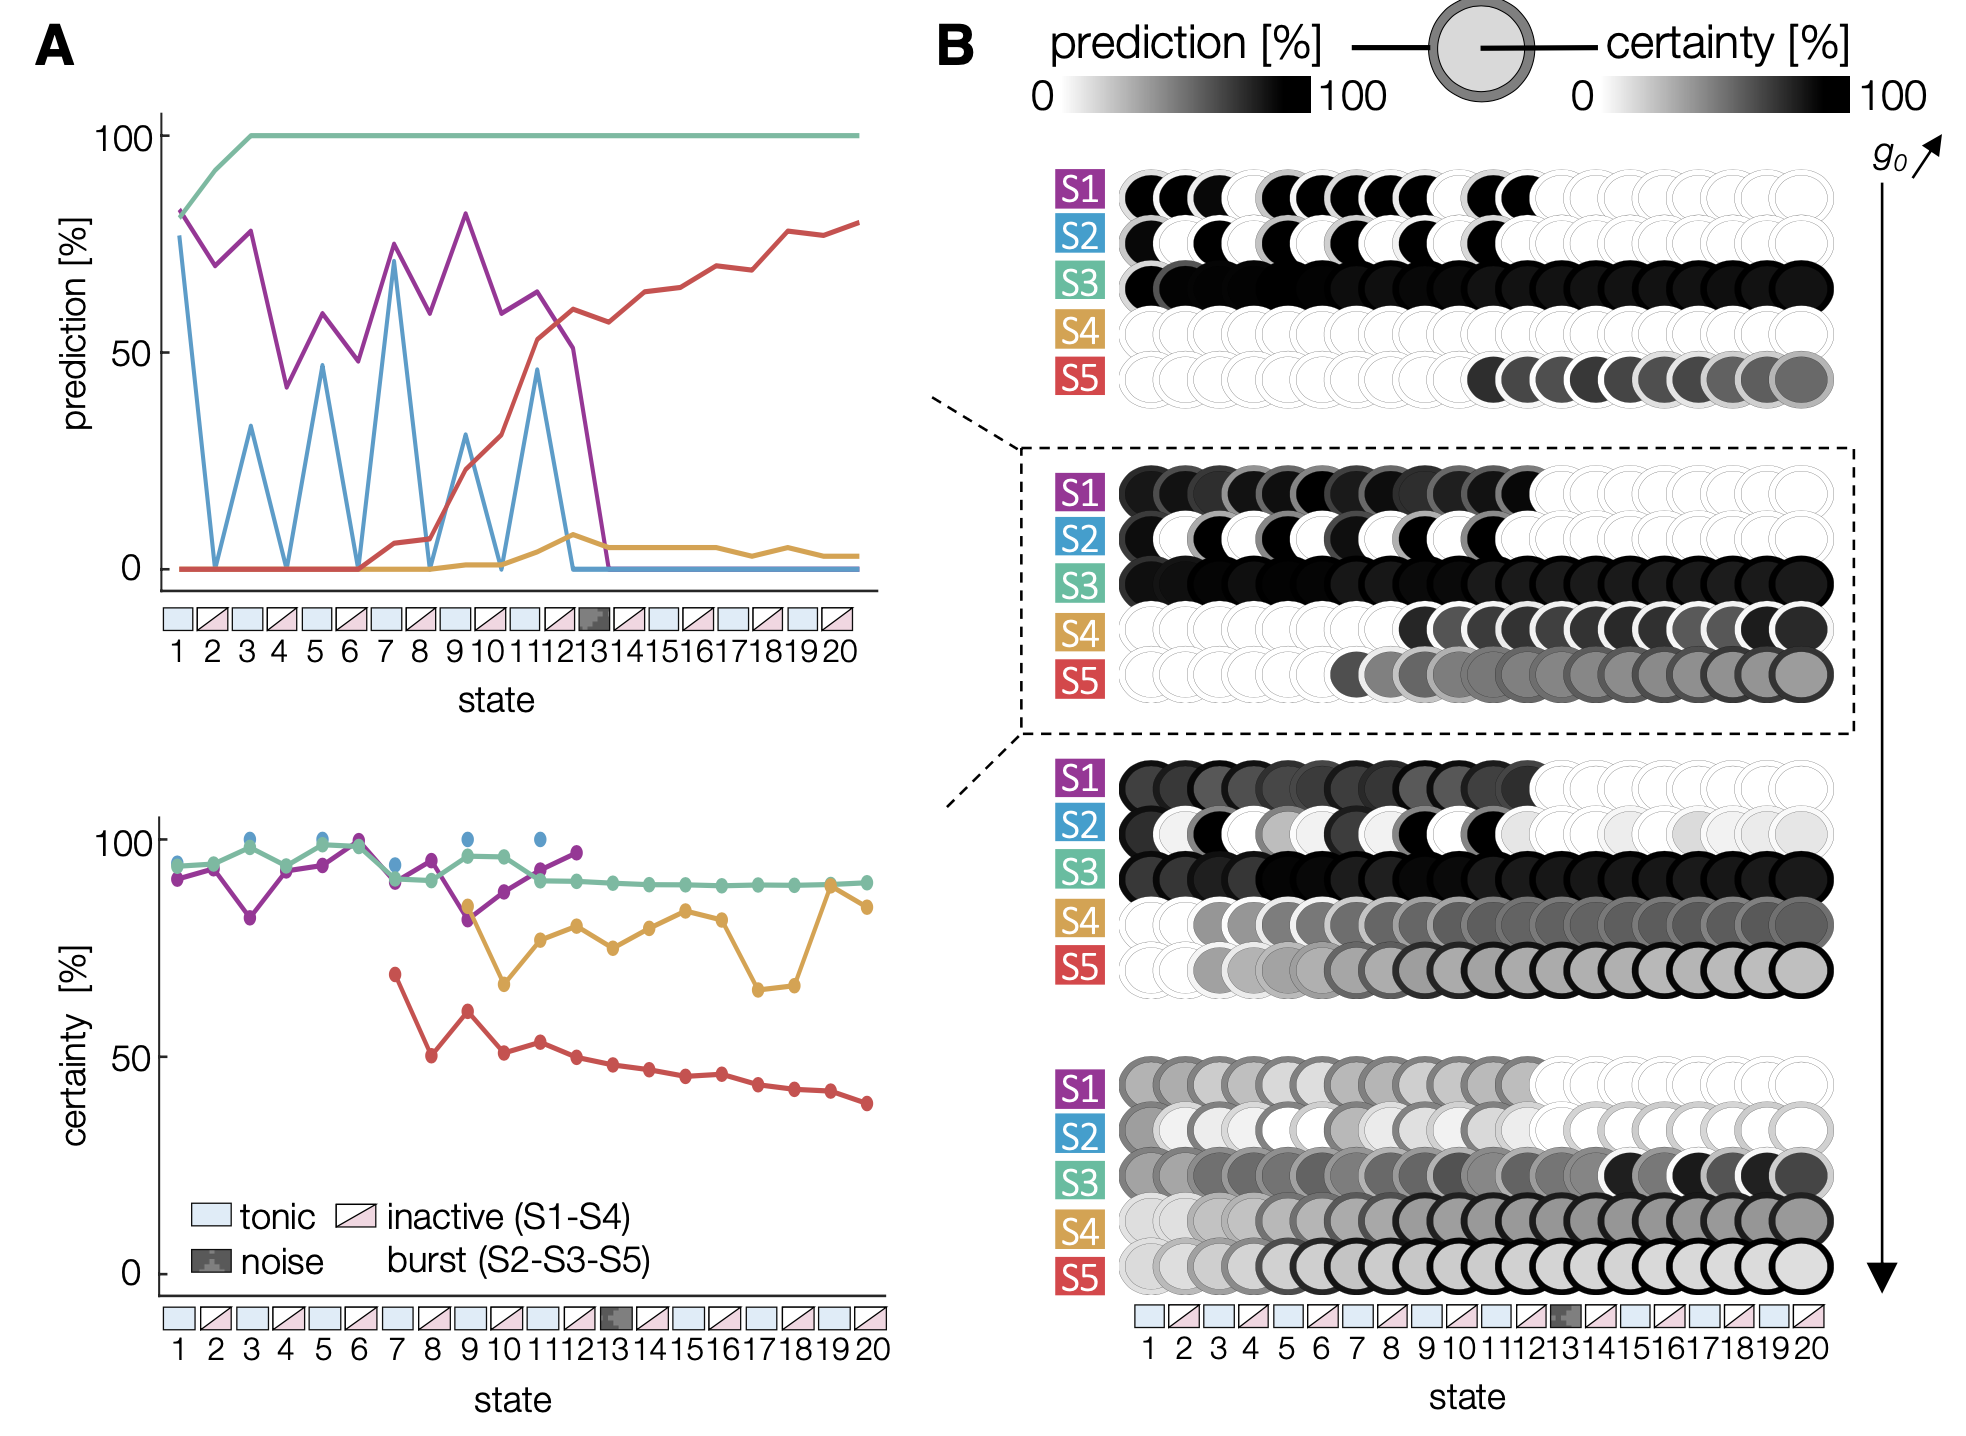
\includegraphics[scale=0.4]{fig/Task/Fig3_flake.png}
    \caption{Caption}
    \label{fig:Task_3_flake}
\end{figure}



% ---------------------------------------
%       RESULT 4: MNIST 
% ---------------------------------------
In the third memory task, we implement a more complex pattern recognition task using a reduced MNIST dataset \citep{garg_voltage-dependent_2022}. Again, we use tonic learning states interleaved with either inactive (S1) or bursting states (S2-S3). The \textit{receptive field} is defined as a weight matrix associated with each output neuron, which indicates the relative weights assigned to the input neurons contributing to that neuron's activation. We show the evolution of the receptive field of the output neuron associated to the digit 0 \textcolor{red}{modifier pour montrer tous les receptive fields}. We find that in S1, the receptive field is affected by each tonic firing learning state and entirely destroyed when a noisy image is presented. In S2, the receptive field resets at each bursting state as before. However, in S3, where learning is transferred from the synaptic efficacy to synaptic conductance, the receptive field is consolidated at each state and is robust to noise. 


% ---------------------------------------
%       RESULT 5: CONNECTIVITY 
% ---------------------------------------
\textcolor{red}{est-ce qu'on parle de ca ? }

% -------------------------------
% -------------------------------
%
%           DISCUSSION
%
% -------------------------------
% -------------------------------

\section{Discussion}
\subsection{Discussion 1}
\textcolor{blue}{COSYNE}\\
In summary, we show that traditional plasticity rules suffer from forgetting through burst-dependent reset but structural plasticity rescues memory and, combined with burst-induced reset, provides a robust mechanism for consolidation. Importantly, the results from our simple memory tasks make quantitative experimental predictions for the role of bursting states during learning. Finally, our work suggests incorporating structural plasticity and distinct tonic/bursting states for more reliable learning performance in artificial neural networks for machine learning applications. 



\textcolor{blue}{OCNS}\\
Overall, we demonstrate that while traditional plasticity rules enable learning during tonic states, they also result to forgetting due to homeostatic reset during bursting states. On the other hand, burst-driven structural plasticity salvages memory and, in combination with the homeostatic reset, provides a robust mechanism for consolidation. Moreover, when bursting states are replaced by inactive states, learning can be maintained but the SNR becomes saturated, memory consolidation is not achieved, and the network becomes vulnerable to noise (S1). Importantly, our results, which are based on simple memory tasks, generate quantitative experimental predictions for the role of bursting in learning. This confirms that synaptic plasticity is a complex process that operates on different timescales to facilitate memory formation and consolidation during switches in neuronal activity. Ultimately, our study suggests incorporating structural plasticity and distinct tonic/bursting states for more reliable learning performance in artificial neural networks, particularly in machine learning applications. 


\subsection{Limitations of the burst-dependent structural plasticity}
\textcolor{blue}{new}\\
Discuss the assumption made that $g$ is modified only during bursting rhythm and not in the other states. (i) justify with neuromodulator states, (ii) say that it is an assumption and to improve the structural plasticity, the synaptic conductance must change depending on internal state variable such as calcium for example. (iii) use a structural plasticity that is governed by $\dot{w}$ to avoid predicting the value of the reset. 


\section{Papers intéressants pour l'article}
- \citep{brokaw_resting_2016} "These observations suggest that a short period of quiet rest can facilitate memory consolidation processes."
- \textcolor{red}{retrouver l'article de Alessio qui montre que sans burst on n'a pas d'apprentissage}




%-------------- Conclusions
%\chapter{Conclusions and Prospect}


\section{Intrinsic plasticity}


\section{Machine learning}
NMOD: \citep{mei_informing_2022}\\
sleep on network: \url{https://www.snexplores.org/article/sleep-ai-models-learning-new-things-computer-memory}\\
switches: article de aurélien (TFE) \\

\section{Sleep-Dream}
creativity: \citep{lacaux_increased_2019} : papier super intéressant sur l'augementation de la créativité pendant le sommeil (preuve avec des patients narcoleptiques)




%-------------- Side Projects
%\section{Project with Kevin}
\section{Patch clamp with Vincent}
\section{Project with Montpellier}
\section{My master thesis students}



%-------------- SI
%\chapter{Supplementary Materials}
\section{The brain and its main structures}
\begin{itemize}
 \item \textit{basal ganglia}: collection of structures located deep within the brain that are involved in the control of movement, particularly in the initiation and suppression of movements.
 \item the \textit{striatum}: involved in the control of movement, it sends output to the motor cortex. 
 \item  \textit{brainstem} composed of the midbrain, pons and medulla, it connects the brain to the spinal cord
 the \item the \textit{locus coeruleus} (inside the pons, involved in the regulation of attention and arousal. It releases the neurotransmitter norepinephrine, which can modulate the activity of other brain regions).
 \item the \textit{basal forebrain} (involved in the regulation of attention, learning, and memory. It contains several different nuclei that release the neurotransmitter acetylcholine)
 \item the \textit{nucleus basalis of Meyner} (The nucleus basalis of Meynert is a group of neurons located in the basal forebrain that release acetylcholine and play an important role in attention and memory)
 \item the \textit{amygdala} (in the temporal lobe, involved in the processing of emotions, particularly fear and anxiety)
 \item the \textit{raphe nuclei} (collection of nuclei located in the brainstem that release the neurotransmitter serotonin. They are involved in the regulation of mood, sleep, and appetite)
 \item the \textit{substantia niagra} (structure located in the midbrain that is involved in the control of movement. It releases the neurotransmitter dopamine, which is important for the initiation and control of voluntary movements.)
 \item the \textit{ventral tegmental area} (The ventral tegmental area is a group of neurons located in the midbrain that release dopamine and play an important role in reward processing and motivation.)
 \item the \textit{hypothalamus} (small structure located near the base of the brain that plays a crucial role in regulating many physiological processes, such as hunger, thirst,).
\end{itemize}


\newpage
% ----------------------------------------------
% ----------------------------------------------
%
%
%               PHASE PLANE ANALYSIS
%
%
% ----------------------------------------------
% ----------------------------------------------

\section{Phase plane analysis: a powerful tool}
\subsubsection{Mathematical reminders}
This section is a general toolbox to understand non-linear systems analysis, based on the manuscript I wrote for the lecture 'Introduction to signals and systems' (fr: introduction aux signaux et systèmes, a lecture taught in second year of Bachelor at the Faculty of Applied Sciences at the University of Liège) \textcolor{red}{REF}. 

We start with a non-linear system of two variables $x_1$ and $x_2$ such as : 
\begin{equation*}
\left\{
    \begin{array}{lllllll}
        \dot{x}_1 &=& f_1(x_1,x_2)\\
        \dot{x}_2 &=& f_2(x_1,x_2) 
    \end{array}
\right.
\end{equation*}
\textbf{Graphical analysis in the phase plane}\\
Without solving complicated math, the phase plane allows to understand globally the dynamics of the systems. The phase portrait is a 2D plane and the horizontal axis is associated with the $x_1$ and the vertical axis is $x_2$.

We define the \textit{nullclines} which are defined as the locus of points where one of the derivative is null:
\begin{equation*}
\left\{
    \begin{array}{lllllll}
        x_1\mbox{-nullcline}: \dot{x}_1 =0 \rightarrow f_1(x_1,x_2) = 0  \\
        x_2\mbox{-nullcline}: \dot{x}_2 =0 \rightarrow f_2(x_1,x_2) = 0 \\
    \end{array}
\right.
\end{equation*}
The intersections between the two nullclines where $\dot{x}_1=0$ and $\dot{x}_2=0$ simultaneously defines the \textit{fixed points}: $(x_1^*,x_2^*)$. 

At each point on the plane, we can compute
\begin{equation*}
\left\{
    \begin{array}{lllllll}
        \dot{x}_1^* &=& f_1(x_1^*,x_2^*)\\
        \dot{x}_2^* &=& f_2(x_1^*,x_2^*) 
    \end{array}
\right.
\end{equation*}
where $\dot{x}_1^*$ gives the horizontal velocity and  $\dot{x}_2^*$ gives the vertical velocity. The resulting vector is the velocity at the given point in the plane. We can draw these vectors for plenty of points in the plane which brings out the \textit{vector field}. By analogy, we imagine a piece of wood on a water, the vector field simply provides the direction of the current, the fixed points are locations where the piece of wood remains fixed. 

To determine the stability of the fixed points, we watch the direction of the fields. When all the lines converge towards this point, it is a \textit{stable} fixed point. By contrast, if all the line diverge, it is a \textit{unstable} fixed point. We can also differenciate if the lines rotates towards the fixed points; it defines a stable spirale while if its direclty converges towards the point it is stable node. A similar reasoning permits to observe unstable spirale or unstable node. We can also define limit case such as center where the vector field is never converging and diverging from the node and saddle node where the vector field is attracted in one direction and repulse in the other direction. 

As you can see, this analysis provides a good way to study non linear system without solving all the differential equations and without doing any computations. \\
~\\
\textbf{Analytical analysis in the phase plane}\\
We can also determine the stability of the phase plane via analytic computations. We introduce the Jacobian matrix: 
\begin{align*}
    A &=  \begin{pmatrix}  \dfrac{\partial f_1}{\partial x_1} & \dfrac{\partial f_1}{\partial x_2} \\  \dfrac{\partial f_2}{\partial x_1} & \dfrac{\partial f_2}{\partial x_2}  \end{pmatrix}
\end{align*}

Then the eigenvalues of the Jacobian evaluated at the fixed points give the nature and stability of the fixed points. Here we consider a 2D system, the stability can be determined based on the determinant and the trace of the jacobian following Figure \ref{fig:strogatz}.

\begin{figure}[h!]
    \centering
    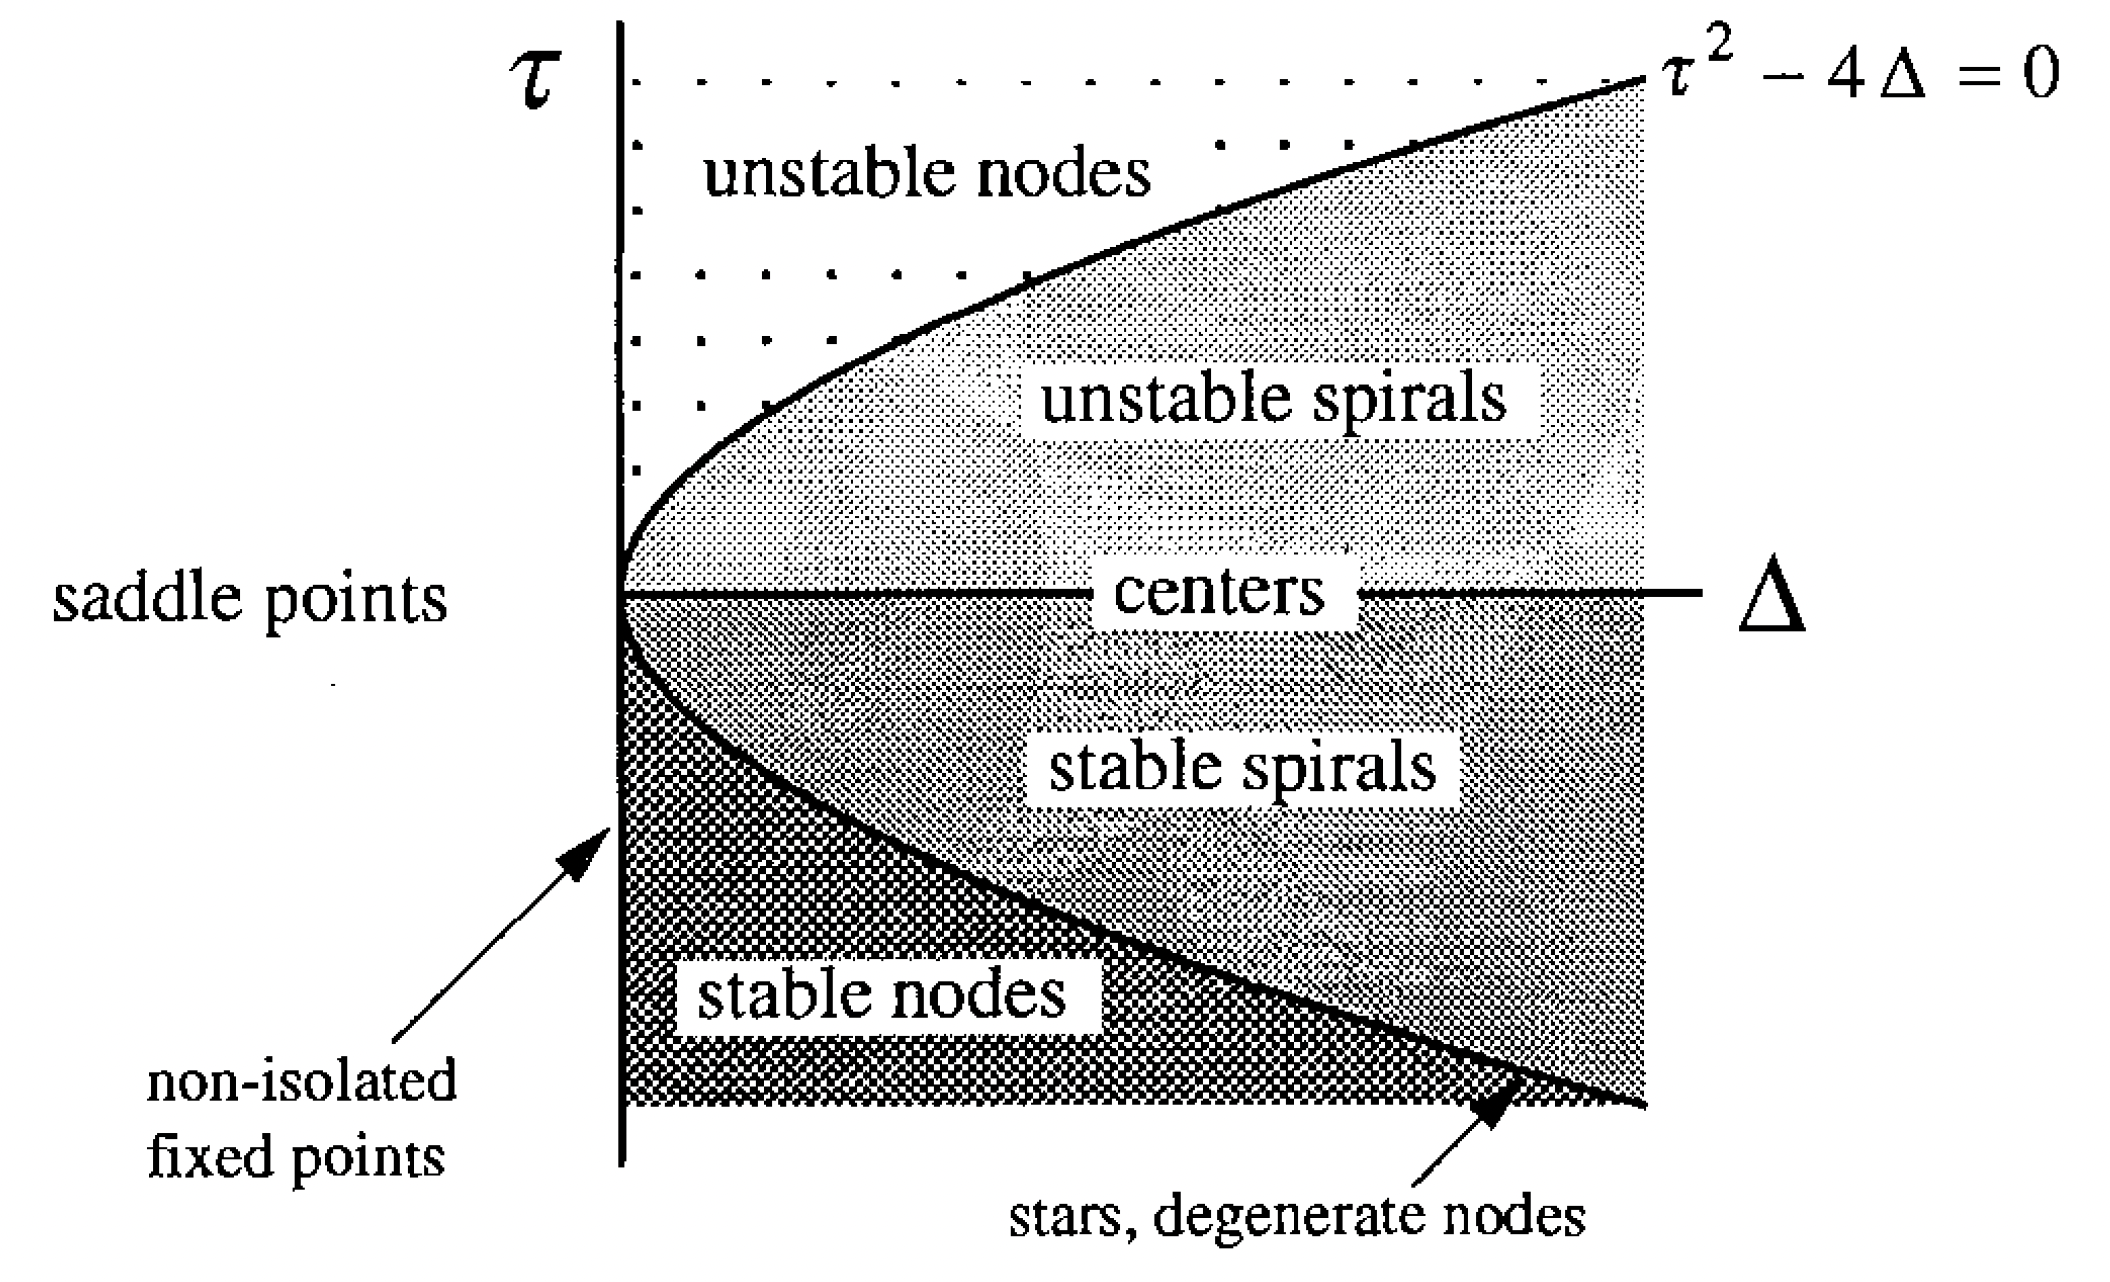
\includegraphics[scale=0.3]{latex/fig/Methods/Strogatz.png}
    \caption{The stability of the fixed points in a 2D system is defined by the values of the trace ($\tau$) and the determinant ($\Delta$) of the jacobian evaluated at the fixed points \citep{strogatz_nonlinear_2015}}
    \label{fig:strogatz}
\end{figure}


\begin{pinkshaded}
\begin{center}
\textbf{Notions clés}\\
\end{center}
~\\
\begin{tabular}{l| l l}
    Approche &\textbf{Globale | Graphique}  & \textbf{Locale | Mathématique} \\
     &tracer $\dot{x} = f(x)$ & équation $\dot{x} = f(x)$ \\
    Points fixes & intersection avec l'axe x & résoudre équation:$f(x)=0 \rightarrow x^*=...$\\
    Stabilité & tracer le champ de vecteur & étudier le signe de la dérivée première \\
    & $\dot{x}>0: \rightarrow$& (i) calcul $f'(x)$\\
    & $\dot{x}<0: \leftarrow$& (ii) remplacer $x$ par $x*$: $f'(x^*)$\\
    \textit{stable} &     $\rightarrow \bullet \leftarrow$ &  $f'(x^*)<0$ (pente négative)\\
    \textit{instable}&    $\leftarrow \circ \rightarrow$ &  $f'(x^*)>0$ (pente positive)\\
\end{tabular}
\end{pinkshaded}



% -------------------------
%
%
%       SI Article PLOS
%
%-------------------------

\begin{comment}
\chapter{Supplementary Materials}

\section{Plos Article}
\section*{Supporting information}

% Include only the SI item label in the paragraph heading. Use the \nameref{label} command to cite SI items in the text.

\paragraph{S1}
\label{S1_Video}
{\bf Video. Membrane voltage evolution during a hyperpolarized-induced bursting (top) and its associated phase portrait considering a \textit{fast} activation of T-type calcium channel (bottom).} V-(resp. V-s) nullcline is skteched in blue (resp. green).  The trajectory is marked by round circles. The simulation is shown for the reduced model 1 (Video associated to Fig~\ref{fig:6} (left)).

\paragraph{S2}
\label{S2_Video}
{\bf Video. Membrane voltage evolution during a hyperpolarized-induced bursting (top) and its associated phase portrait for a \textit{slow} activation of T-type calcium channel (bottom).} V-(resp. V-s) nullcline is skteched in blue (resp. green).  The trajectory is marked by round circles. The simulation is shown for the reduced model 1 (Video associated to Fig~\ref{fig:6} (center)).

\paragraph*{S3}
\label{S3_Video}
{\bf Video. Membrane voltage evolution during a hyperpolarized-induced bursting (top) and its associated phase portrait for a \textit{ultraslow} activation of T-type calcium channel (bottom).} V-(resp. V-s) nullcline is skteched in blue (resp. green).  The trajectory is marked by round circles. The simulation is shown for the reduced model 1 (Video associated to Fig~\ref{fig:6} (right)).

\paragraph{S4}
\label{S4_Video}
{\bf Video. Phase portrait evolution as a function of the T-type calcium channel activation kinetics } V-(resp. V-s) nullcline is skteched in blue (resp. green). The multiplicative factor of the T-type calcium channel activation time constant is indicated by $\eta$.  Apparition of the lower branch in the V-nullcline when the activation decelerates. Then, the lower branch disappears into a hourglass shape. Results shown for the reduced model 1. Similar phase portraits evolution of the reduced models 2, 5' and 6' are available on \url{http://www.montefiore.ulg.ac.be/~guilldrion/Files/Jacquerie2021_codes.zip} (in the folder "video").

\paragraph*{S5}
\label{S5_Video}
{\bf Video. Membrane voltage evolution during a hyperpolarized-induced bursting (top) and its associated phase portrait at the nominal value of the membrane capacitance (bottom).} V-(resp. V-s) nullcline is skteched in blue (resp. green).  The trajectory is marked by round circles (Video associated to Fig~\ref{fig:7}A (left)).

\paragraph*{S6}
\label{S6_Video}
{\bf Video. Membrane voltage evolution during a hyperpolarized-induced bursting (top) and its associated phase portrait when the membrane capacitance is scaled by 1/3 (bottom).} V-(resp. V-s) nullcline is skteched in blue (resp. green).  The trajectory is marked by round circles (Video associated to Fig~\ref{fig:7}A (right)).

\paragraph*{S7}
\label{S7_Video}
{\bf Video. Membrane voltage evolution during a hyperpolarized-induced bursting (top) and its associated phase portrait at the nominal value of the membrane capacitance (bottom).} V-(resp. V-s) nullcline is skteched in blue (resp. green).  The trajectory is marked by round circles (Video associated to Fig~\ref{fig:7}B (left)).

\paragraph*{S8}
\label{S8_Video}
{\bf Video. Membrane voltage evolution during a hyperpolarized-induced bursting (top) and its associated phase portrait when the membrane capacitance is scaled by 1/3 (bottom).} V-(resp. V-s) nullcline is skteched in blue (resp. green).  The trajectory is marked by round circles (Video associated to Fig~\ref{fig:7}B (right)).




\paragraph*{S1}
\label{S1_Supplementary_Material}
{\bf Supplementary Material.} \textbf{A:} Quantification of the firing pattern properties. \textbf{B:}  Simulation of the reduced models not exhibited in the Results.  \textbf{C:} Model description and their parameter values.  \textbf{D:} 
Ionic channel description: steady-state functions and time constants of the gating variables.  \textbf{E:} Description of reduced models and their parameter values. 
\end{comment}

\newpage

%-------------- Biblio
\bibliography{neuro_lab.bib}

\end{document}